%%% Time-stamp: <2015-04-15 00:55:14 sunthar>

%%% $Log:$

%\documentclass[11pt,a4paper,openright]{report}
\documentclass[seminar,twoside]{iitbreport}


%% Selectively comment out sections that you want to be left out but
%% maintaining the page numbers and other \ref
\includeonly{%
 % intro/introduction,
 % lit/literature,
  methods/methods,
 % expt/experimental,
 %expt/VOF_Benchmark,
 % rnd/results
}

%%% Some commonly used packages (make sure your LaTeX installation
%%% contains these packages, if not ask your senior to help installing
%%% the packages)




\usepackage{booktabs}
\graphicspath{{images/}}
\usepackage{subfig}
\usepackage{tabularx}


%%% Macro definitions for Commonly used symbols
\newcommand{\etas}{\ensuremath{\eta_{\mathrm{s}}}}
\newcommand{\Rey}{\ensuremath{\mathrm{Re}}}
\newcommand{\avg}[1]{\ensuremath{\overline{#1}}}
\newcommand{\tenpow}[1]{\ensuremath{\times 10^{#1}}}

\newcommand{\pder}[2]{\ensuremath{\frac{\partial#1}{\partial#2}}}


% Referencing macros
\newcommand{\Eqref}[1]{Equation~\eqref{#1}}
\newcommand{\Tabref}[1]{Table~\ref{#1}}
\newcommand{\Figref}[1]{Figure~\ref{#1}}
\newcommand{\Appref}[1]{Appendix~\ref{#1}}



\begin{document}
\title{Droplet Impact Dynamics}
\author{Palas Kumar Farsoiya \\ (Roll No: 144026002 )}
%\date{\today}
\degree{Doctor of Philosophy}
\dept{Chemical Engineering}
\monthyear{April 2015}

%\makecoverpage
\maketitle
%\begin{center}
\textbf{\large Acknowledgement} 
\end{center}
\indent \\
\indent I would like to acknowledge my supervisor Prof. Ratul Dasgupta for providing me VOF code for further developement. Further, he has appreciated me in developing concepts and manifesting them in codes. He has time to time monitored my progress and provided with valuable aids in terms of suggestions, resources, lectures and even disagreement. His efforts have enormously benefited me.\\
\indent I would also like to thank all my friends and lab mates for providing their valuable insights, friendly guidance and support whenever required. I would like to acknowledge Manoj (Doctoral student, IIT Hyderabad) to help me in Gerris simulations.\\
\indent My wonderful family, which has been my constant source of motivation and inspiration. \\
\\
\\
\indent
Thank you
\vspace*{1.6cm}

%\begin{flushright}
Palas Kumar Farsoiya\\
\indent (124020001)
%\end{flushright}

%\begin{center}
\underline{\textbf{\large ACCEPTANCE CERTIFICATE}} \\[1cm]
Seminar Report \\[0.2cm]
Department of Chemical Engineering \\
Indian Institute of Technology, Bombay \\[7.5mm]
\end{center}
%\vspace*{0.75cm}
The Seminar report titled \textbf{Droplet Impact Dynamics} submitted by Palas Kumar Farsoiya (Roll No. 144026002) may please be accepted for being evaluated.\\[1cm]
%\vspace*{1cm}
%\begin{flushright}
\underline{\hspace{4cm}}\\
Prof. Ratul Dasgupta\\
(Research Supervisor)
%\end{flushright}

\begin{abstract}
 Droplet impingement is very common phenomenon in the world around us. This can be seen in the nature as well as in the industries. It is well known
 that the droplets are formed when there are instabilities such as Rayleigh-Plateau instability, but it is not easy to predict the complex dynamics of droplets. Droplet impact 
 on a solid surface is one such phenomena which intrigues physicsts, mathematicians and engineers. For physicsts the interest lies in understanding the solution of Navier-stokes
 equation before and after impact and various intricacies of the boundary conditions on the dry rigid surface,  mathematicians study the asymptotic solution of the governing laws
 of the fluid dynamics and for engineers, droplet impact is of tremendous technolgical importance as its application lies in silicon chip techology, ink jet printing, internal combustion engines, spray painting and coating,
 plasma spraying and crop spraying. This report presents with a short review on the droplet impact and a numerical study of droplet impact applying simple contact line and contact angle
 models.
\end{abstract}

\pagenumbering{roman}
\tableofcontents

\listoftables
\listoffigures

\cleardoublepage
\setcounter{page}{1}
\pagenumbering{arabic}

%
\chapter{Introduction and Literature Review}
\section{Introduction}
Droplet impact is a phenomenon which is prevalent in many industrial processes such ink-jet printing, 
spray cooling of hot surfaces. Microelectronic industries uses precision solder drop dispensing to produce
electric circuits. Aircraft and power distribution lines encounter accumulation of ice involving droplet impact.
Natural phenomena such as rain effects the aeration of lakes, seas and oceans. 
Forensic science necessitates development of non-wettable and fully wettable surfaces. Criminalistics involves
reconstructing crime scenes in which it is need to study the stain patterns of blood drops impacting surfaces.
With a rising world population, there is huge rise in agricultural growth and use of pesticides is necessary. Pesticides spray 
on crops is also an application which exhibits droplet impact on the plants where spreading of droplets is necessary. 
\begin{figure}[tbp]
 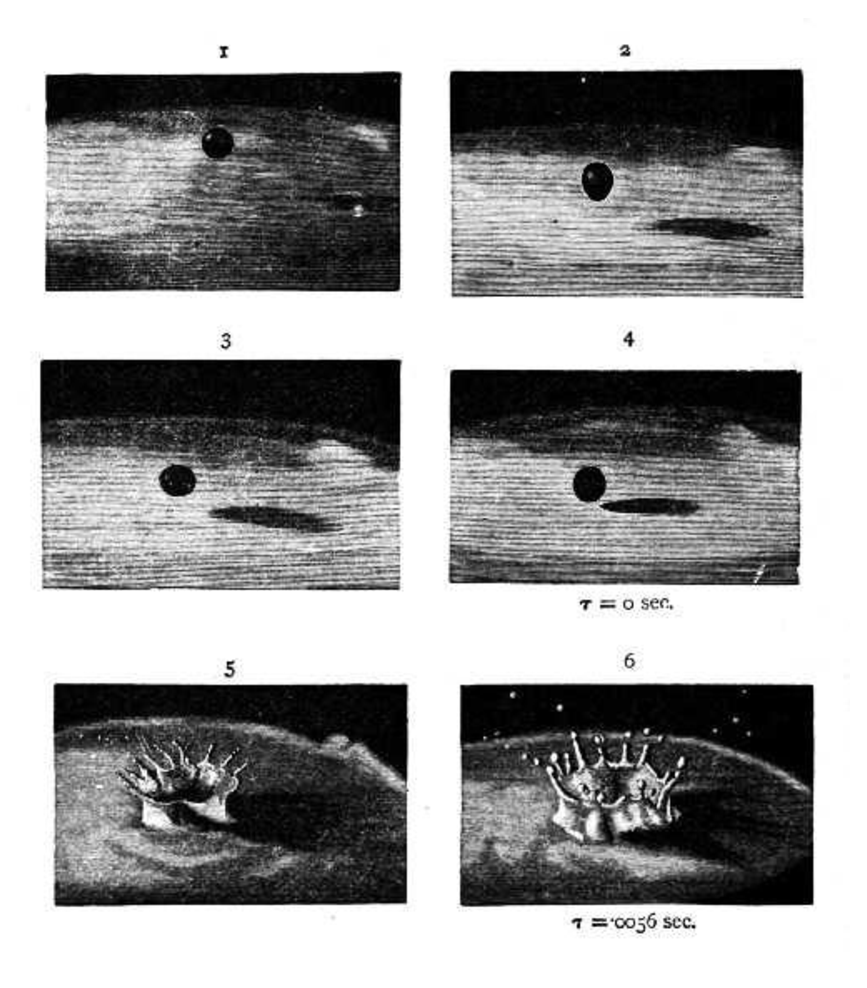
\includegraphics{worthington.eps}
 \caption{Droplet impact graphic by \cite{Worthington1908}}
\label{Fig:Worthington}
\end{figure}


The scientific literature on drops starts with the droplet formation which was studied by many scientists while studying the
free surface flow. The first scientific observation on drops can be found in the book by \cite{Mariotte1700} on motion of  
fluids. They observed that water flowing through the hole of a container bottom breaks into drops. \cite{Taylor1963} solved the  axisymmetric Navier-Stokes  using
singular perturbation method for a drop/bubble in an unbounded fluid. Droplet impact was first investigated experimentally by \cite{Worthington1908} (See Figure \ref{Fig:Worthington}).
The area of droplet formation has also been researched extremely by scientists working in the non-linear dynamics.

The dynamics of the impinging drop is complex and hence many aspects are not understood well. For example, droplets falling
on a surface can undergo many different modes of deformation. It can splash, bounce or simply deposit on a surface. \cite{Rein2002} 
explained through a cartoon, the various possible outcomes of droplet impact. (See Figure \ref{Fig:rein})

\begin{figure}[tbp]
 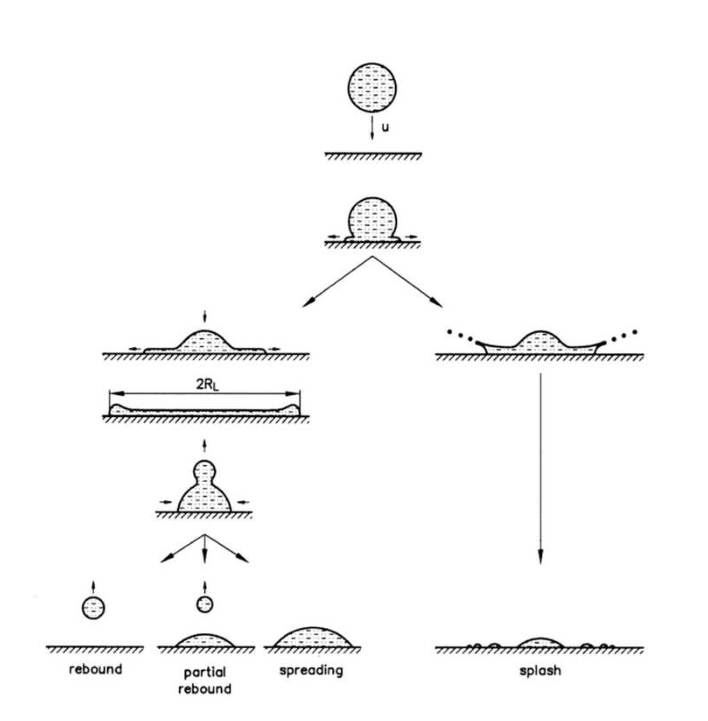
\includegraphics{rein.eps}
 \caption[Different modes of deformation of droplet impact]{Cartoon of different modes of deformation of droplet impact by \cite{Rein2002} }
 \label{Fig:rein}
\end{figure}

%
\section{Literature Review of droplet impacts}

Droplet impact has been investigated from more than a century.These studies can be classified into three broad categories :- 
\begin{enumerate}
 \item Experimental Phenomenology.
 \item Simulation.
 \item Theory.
\end{enumerate}

There are many studies which are combination of the two or more as well e.g. \cite{Mao1997} has proposed theoretical models which were supported by experiments. We
begin with a brief discussion on experimental phenomenology.
\subsection{Experimental Phenomenology}
With the advent of high speed photography in late 1800s, it became possible to observe numerous phenomena which were too fast for the human eye.
Having developed the skills of high speed photography, \cite{Worthington1908} captured photographs of droplet impact. Since then various aspects of
droplet impact have being studied. There are now sophisticated digital systems which can record images at a very high frame rate 
(See Figure \ref{gunjal}) that enable us to capture very fast dynamics which are not visible to human eye.
\begin{figure}[tbp]
\centering
 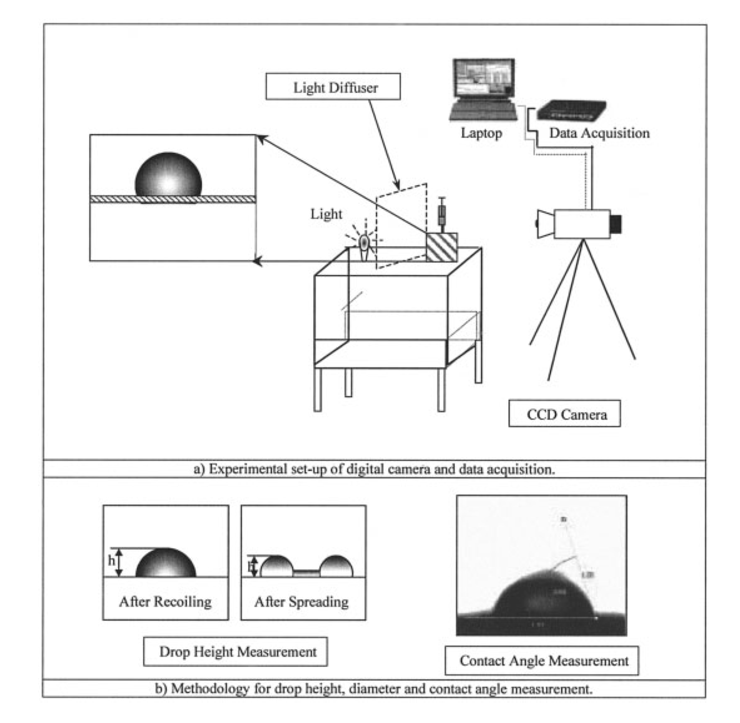
\includegraphics{gunjal.eps}
 \caption[Experimental setup to study droplet impact]{Experimental setup to study droplet impact by \cite{Gunjal2005}}
 \label{gunjal}
\end{figure}
\cite{Richard2000} observed for impact on highly hydrophobic surface (contact angle $ > 170^o$), droplets fully bounce, they 
do not tend to spread (See Figure \ref{richard}). They behaved just like spring but found there was a limit in elasticity due to the transfer
of the part of kinetic energy into the drop vibrations.
\begin{figure}[tbp]
\centering
 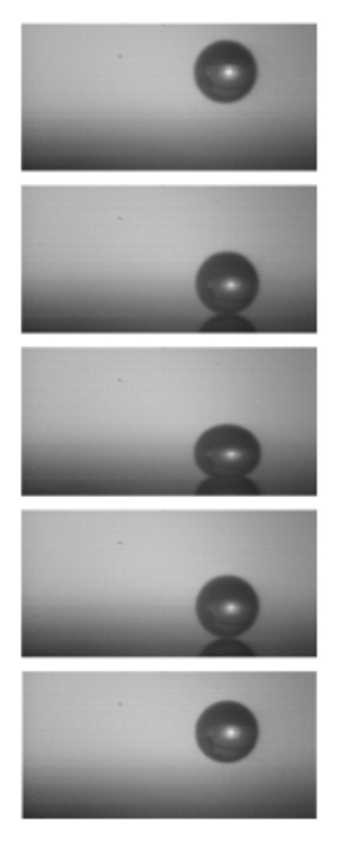
\includegraphics{richard.eps}
 \caption[Droplet impact on superhydrophobic surface]{Droplet impact(R = 0.4 mm) on superhydrophobic surface
 by \cite{Richard2000} }
 \label{richard}
\end{figure}
Droplet impact on dry surfaces are quite different when compared to wet surfaces. \cite{Rioboo2001} studied the effect
various flow parameters and surface characteristics on the droplet impact dynamics. They discovered six different outcomes of a droplet impact on 
a dry surface. In Figure \ref{rioboo} they explained the deposition as droplet deformation and continuous attachment to the surface while spreading without breakup. When
the droplet impacted with a rough surface a splash initiated in the direction of contact line velocity at the onset of spreading called as prompt splash.
Another kind of splash can be seen above the solid surface at the rim of a corona and generally referred to as corona splash.
Sometimes a breakup can be seen while the droplet is receding after maximum spreading, this is attributed to the fact while receding the dynamic contact angle decreases and when 
the limiting value is reached some drops are left behind by the receding lamella. It looks beautiful when a droplet rebounds, this particular process occurs only when a
receding phase  precedes. A full rebound occurs when the dynamic contact angle is large and the receding phases are high in kinetic energy.
\begin{figure}[tbp]
\centering
 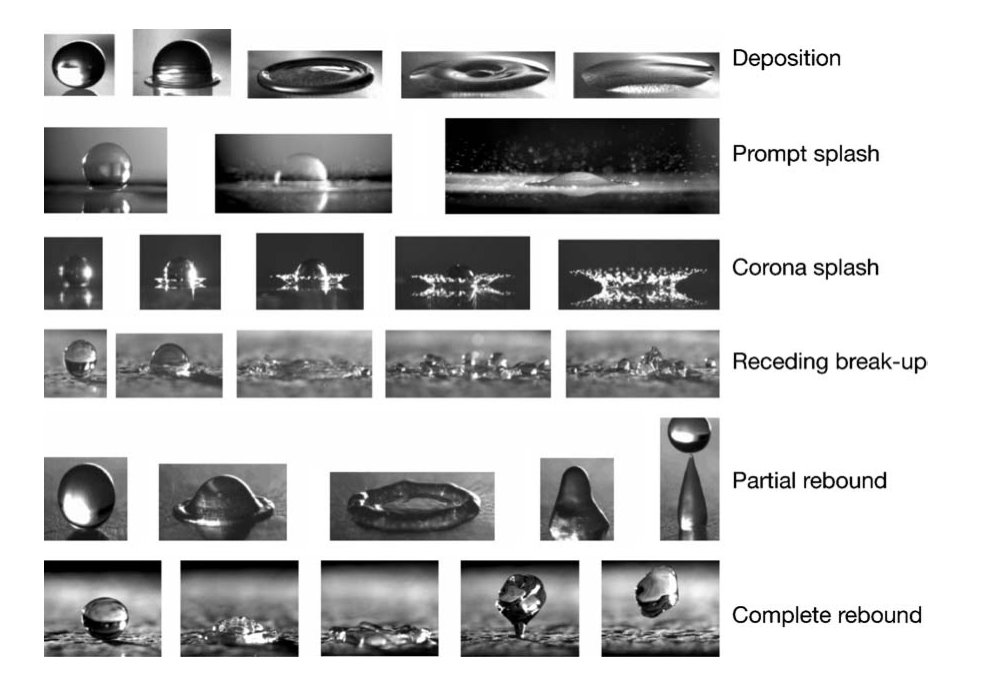
\includegraphics[scale=0.9]{rioboo.eps}
 \caption[Possible outcomes of droplet impact]{Six possible outcomes of droplet impact by \cite{Rioboo2001} }
 \label{rioboo}
\end{figure}
Many scientists have been interested in droplet impact on hydrophobic surfaces. In one such study \cite{Richard2002} found that the contact time of 
bouncing drop does not depend upon the impact velocity of the drop (See Figure \ref{richard2}).
\begin{figure}[tbp]
\centering
 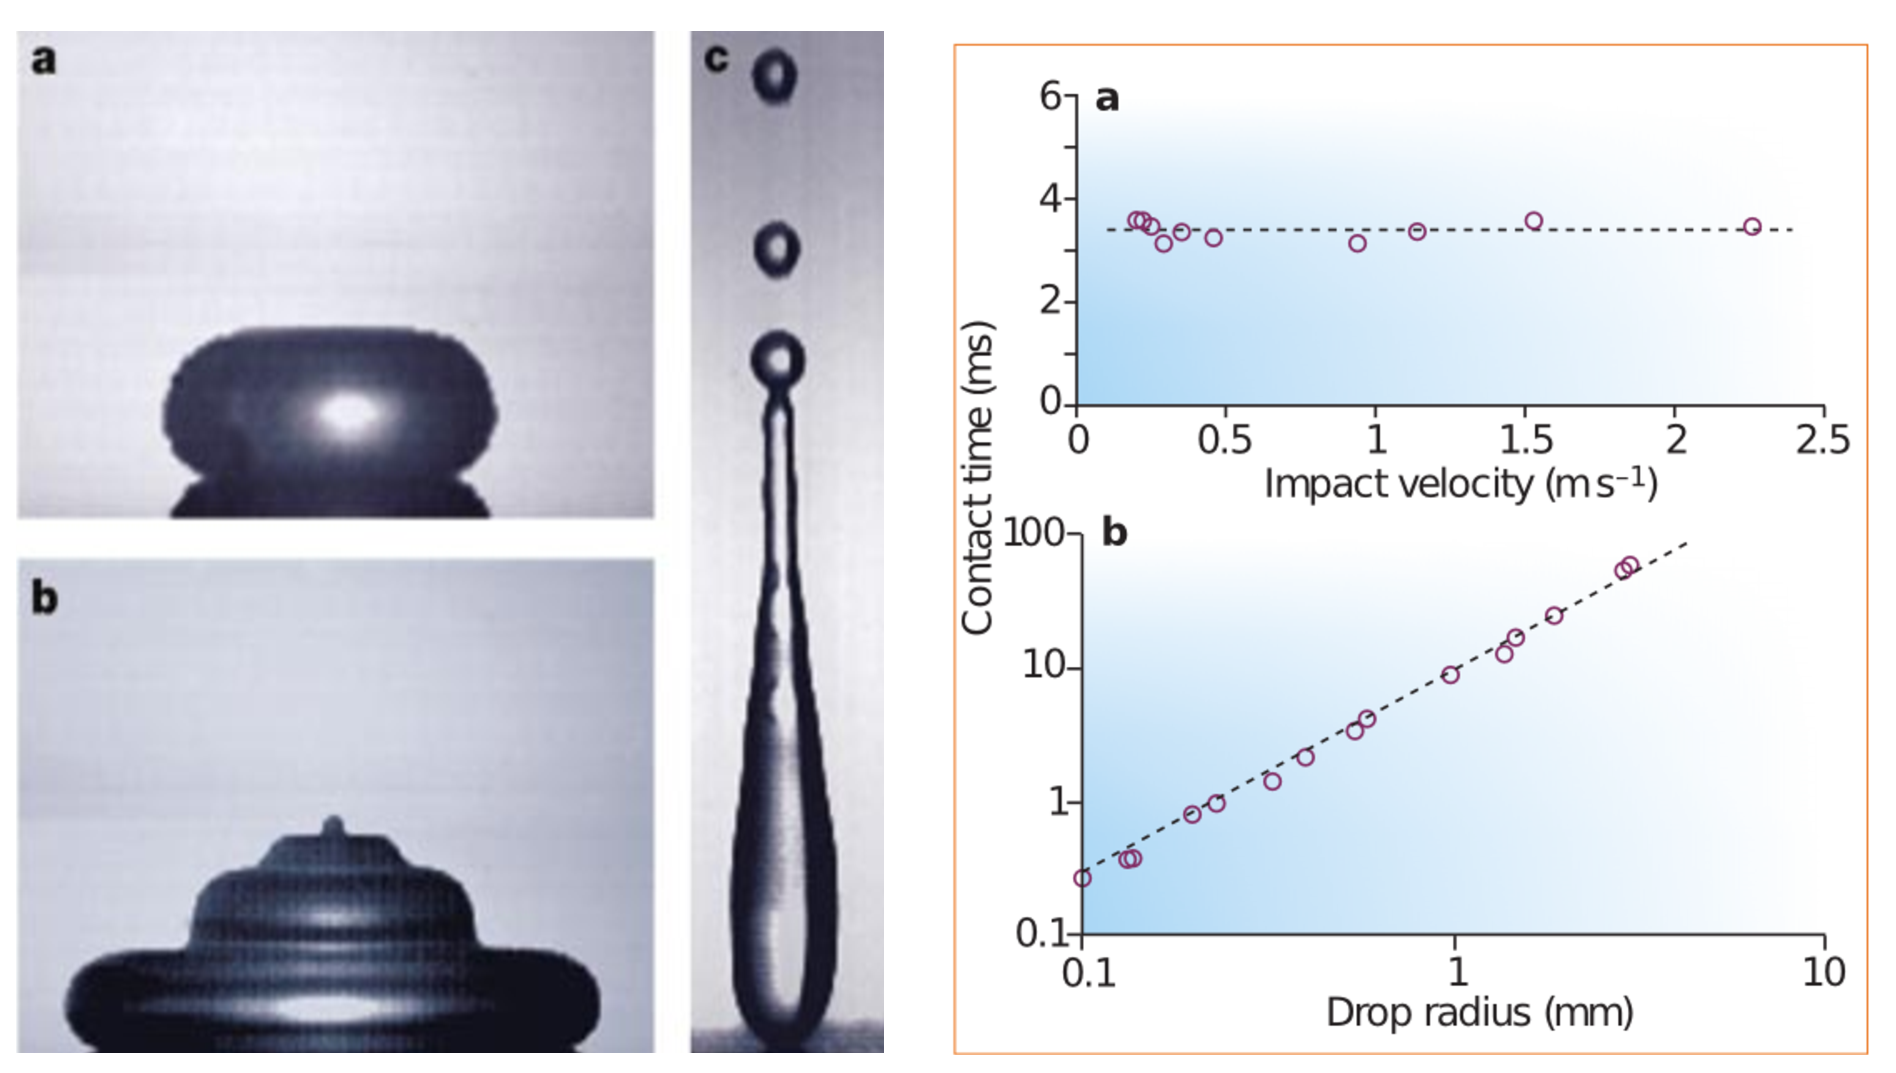
\includegraphics[scale=0.4]{richardc.eps}
 \caption[Contact time of droplet impact on hydrophobic surfaces ]{Contact time of droplet impact on hydrophobic surfaces by \cite{Richard2002} }
 \label{richard2}
\end{figure}
Movement of contact line is a complex phenomena which \cite{Roux2004} studied and obtained an empirical relationship with wetting velocity
of contact line and the impact velocity of the drop. This was later verified by \cite{Hung2011}.
There are a lot of studies on newtonian fluid droplet impact but \cite{Crooks2001} performed some experiments on non-newtonian 
fluids and concluded that the recoil behavior of droplet does not depend on the dynamic surface tension below a critical surfactant
concentration. Here surfactant was added to make the fluid non-newtonian.
\subsection{Simulations}
One of the very early simulation of droplet impact was by \cite{Harlow1967}. They solved the Navier-Stokes equations in cylindrical coordinates in order to
investigate the splash of a drop on a flat plate and deep pool. They used the Marker and Cell {(MAC)} method for interface tracking. The effect of microscopic 
factors such as molecules movement of fluid contact line and surface roughness were also verified by \cite{Gunjal2005} through simulations and experiments. Impact on
inclined surfaces have also received attention in past few years by \cite{Pasandideh1996}, \cite{Kang2000}, \cite{Fukai2000}, \cite{Bussmann1999} and \cite{Sikalo2005}.
These also have been studied by \cite{Lunkad2007} through simulations. \cite{Lunkad2007} applied a Dynamic Contact Angle {(DCA)} model and compared it with Static Contact 
Angle {(SCA)} results, and recommended   {(DCA)} for numerical simulations for better results.

\begin{figure}[tbp]
\centering
 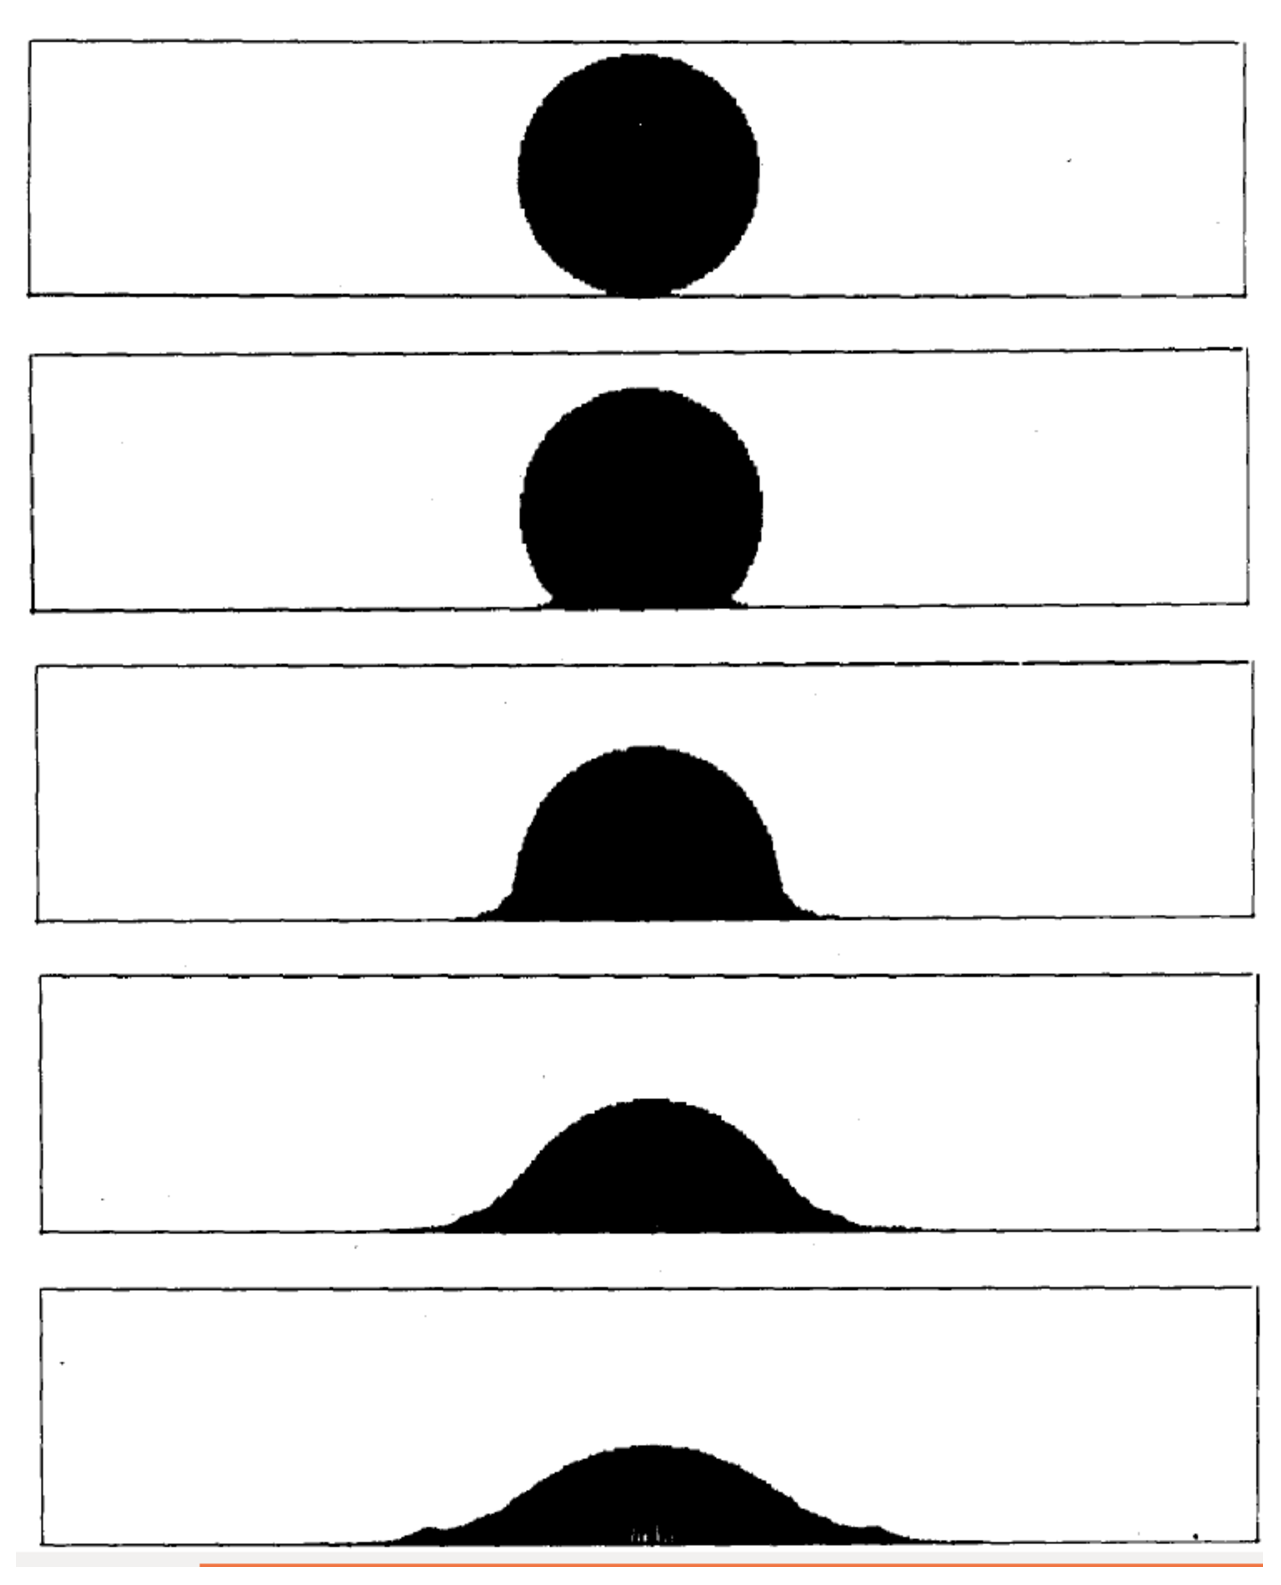
\includegraphics[scale=0.4]{harlow.eps}
 \caption[First numerical study on droplet impact]{The very first numerical study of droplet 
 impact (Reproduced by \cite{Harlow1967} under fair usage policy)}
\end{figure}

\subsection{Theory}
There have been many attempts to explain and model some phenomena which occurs during droplet impact such as 
spread of the droplet after impact. These have been investigated by \cite{Madejski1976}, \cite{Jones1971}, \cite{Chandra1991}, \cite{Scheller1995}, \cite{Bennett1993}, \cite{Pasandideh1996}.
A model was proposed by \cite{Mao1997} for maximum spread as a function of 
 Weber number, Reynolds number, and static contact angle. They also derived a model to predict the rebound by applying conservation of energy, as a function of 
 static contact angle and maximum spread diameter.
Recently a remarkable study by \cite {Liu2015} explained the splashing of droplet on smooth surfaces being due to Kelvin-Helmholtz instability in ultra-thin layer of 
air between the droplet and the surface (See Figure \ref{Fig:liu}).
\begin{figure}
 \centering
 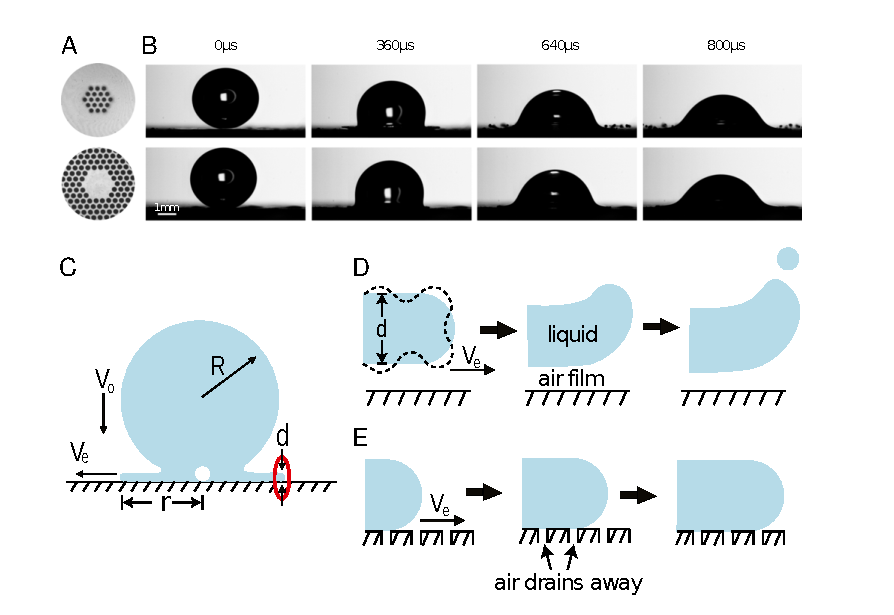
\includegraphics{Liu2015.eps}
 \caption[Kelvin-Helmholtz instability in a droplet splash]{Graphics verifying and explaining the KH instability in the droplet impact which initiates splash (Reproduced by \cite{Liu2015} under fair usage policy)}
 \label{Fig:liu}
\end{figure}

\section{Discussion}
The simulation droplet impact is a complex study as the multiphase solvers must take the effect of surface into the solution. The boundary conditions at the impact surface are non trivial. It
requires understanding of moving contact lines and dynamic contact angles which then has to be implemented in the numerical study. Droplet impact on superhydrophobic surfaces 
however are simpler to study because of the negligible effect of contact line.


    \chapter{Volume of Fluid method}

\section{Introduction}
In this chapter we present the development of in-house code for simulating a two phase flow.
Mathematicians and physicists have studied the dynamics of multiphase flows and as discussed in the previous chapter
literature is quite extensive. Governing equations for such flows are not only nonlinear but the 
position of the interface needs to be found out as a part of solution. Consequently, analytical solutions exist only for very simple problems such as oscillations of bubbles and droplets,
inviscid linear waves and steady state motion of bubbles and droplets in Stokes flow. Thus there is a need for numerical solutions been felt by the multiphase
research community since late fifties and early sixties. 
\cite{Hirt1981} came up with the idea of Volume of Fluid interface {(VOF)} tracking to approximate
the free boundaries in numerical simulations. This method is based on a concept of fractional volume of fluid. This is still widely used due to its flexibility and efficiency
compared to other methods. 
The volume of fluid method conserves mass up to machine accuracy, level set methods conventionally have some issues of mass conservation but
are better in the reconstruction of curved interfaces and thus easier for implementation of surface tension.

\section{The Volume of Fluid method}
This method starts with defining a quantity called as volume fraction F, for each cell in the computational domain. For a binary phase system there is a dark fluid and light fluid.
F is the ratio of volume of the dark fluid to the volume of the cell itself. The cells with only light fluid are chosen to have F = 0 and whereas those with only dark fluid F = 1. For interfacial cells
F will have a value between 0 and 1. The volume of fluid when advected does not change with respect to the fluid parcel. Hence, it satisfies the following relation,

\begin{eqnarray}
\frac{D F}{D t} = 0 
\end{eqnarray}

The Eulerian form would be,

\begin{eqnarray}
 \frac{\partial F}{\partial t}+( u. \nabla)F=0
 \label{Eq:advection_vof}
\end{eqnarray}



As interface in Volume of fluid method can be reconstructed in many ways we choose the Least Squares Volume of 
Fluid Reconstruction Algorithm proposed by \cite{Pilliod2004} which is one of the most accurate algorithm available in literature. It is second order accurate in space 
and can be extended to the 3D. It represents the interface as a line in 2D and a plane in 3D. The VOF method achieves higher accuracy using geometrical techniques to reconstruct
and advect the interface.
Any interface reconstruction algorithm consists two basic steps:-
\begin{enumerate}
 \item Interface Reconstruction
 \item Advection of F field
\end{enumerate}
\pagebreak

\subsection{Interface Reconstruction by Least Squares of Volume of Fluid Interface Reconstruction Algorithm (LVIRA)}
\subsubsection{Step I : Obtain F field}
At first an F-field is obtained by knowing the initial free surface and then by calculating the F values for each cell. 
For reconstruction of interface a cell having a value of F between 0 and 1 is located.

\subsubsection{Step II : Initial guess of slope}
The initial slope of the normal to the interface away from the dark fluid can obtained using (Green-Gauss gradient \cite{Gerlach2006}) which is  given by 
\begin{eqnarray}
  N_x=-\frac{1}{\Delta x}{[F_{r+1,c+1}+2F_{r,c+1}+F_{r-1,c+1}-F_{r+1,c-1}-2F_{r,c-1}-F_{r-1,c-1}]} \\
  N_y=-\frac{1}{\Delta y}{[F_{r+1,c+1}+2F_{r+1,c}+F_{r+1,c-1}-F_{r-1,c+1}-2F_{r-1,c}-F_{r-1,c-1}]}
  \label{Eq:GG}
\end{eqnarray}

\subsubsection{Step III: Quadrant Identification}
To get the interface as a line in 2D, we have to determine its shape and orientation in a cell. First step is to get the normal orientation in the quadrant.
 Signs of $N_x$ and $N_y$ will determine the quadrant in which the normal points away from the dark fluid present in the cell. 
  \begin{figure}%[H]
  \centering
   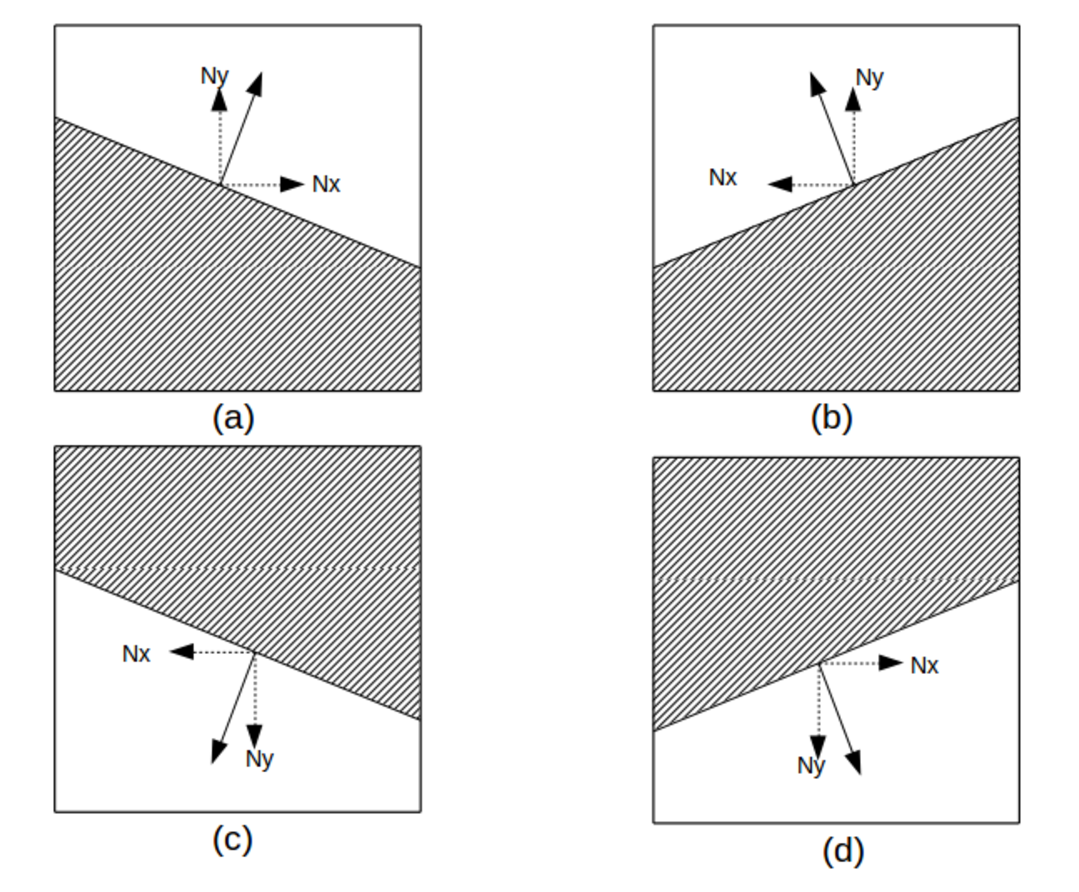
\includegraphics[scale=0.4]{quad.eps}
   \caption[Interface normal direction]{(a)I Quad (b) II Quad (c) III Quad (d) IV Quad }
   \label{Fig:quad}
  \end{figure}

\subsubsection{Step IV: Angle Calculation}
 The angle, $\theta$ is the positive acute angle made by the interface with x-axis if the normal points into first and the third quadrant and positive acute angle made by 
 the interface by y-axis if the normal points into the second and fourth quadrant. This definition is necessary because we treat all other quadrants as the $I^{st}$ quadrant
 by suitable rotation. So for the second and the fourth quadrant $\theta$ has to be redefined. Refer to Figure \ref{Fig:quad} for definition of theta. This is 
 required to do since the algorithm is developed in way it works for normal in first quadrant and all other cases has to be modified according to algorithm.
% 
%  Equation \ref{Eq:angle} gives the expression for calculating $\theta$
% \begin{equation}
%  \theta=\frac{\pi}{2}-tan^{-1}\left(\frac{N_x}{N_y}\right)
%  \label{Eq:angle}
%  \end{equation}
% \begin{wrapfigure}{r}{0.5\textwidth}
%   \begin{center}
%     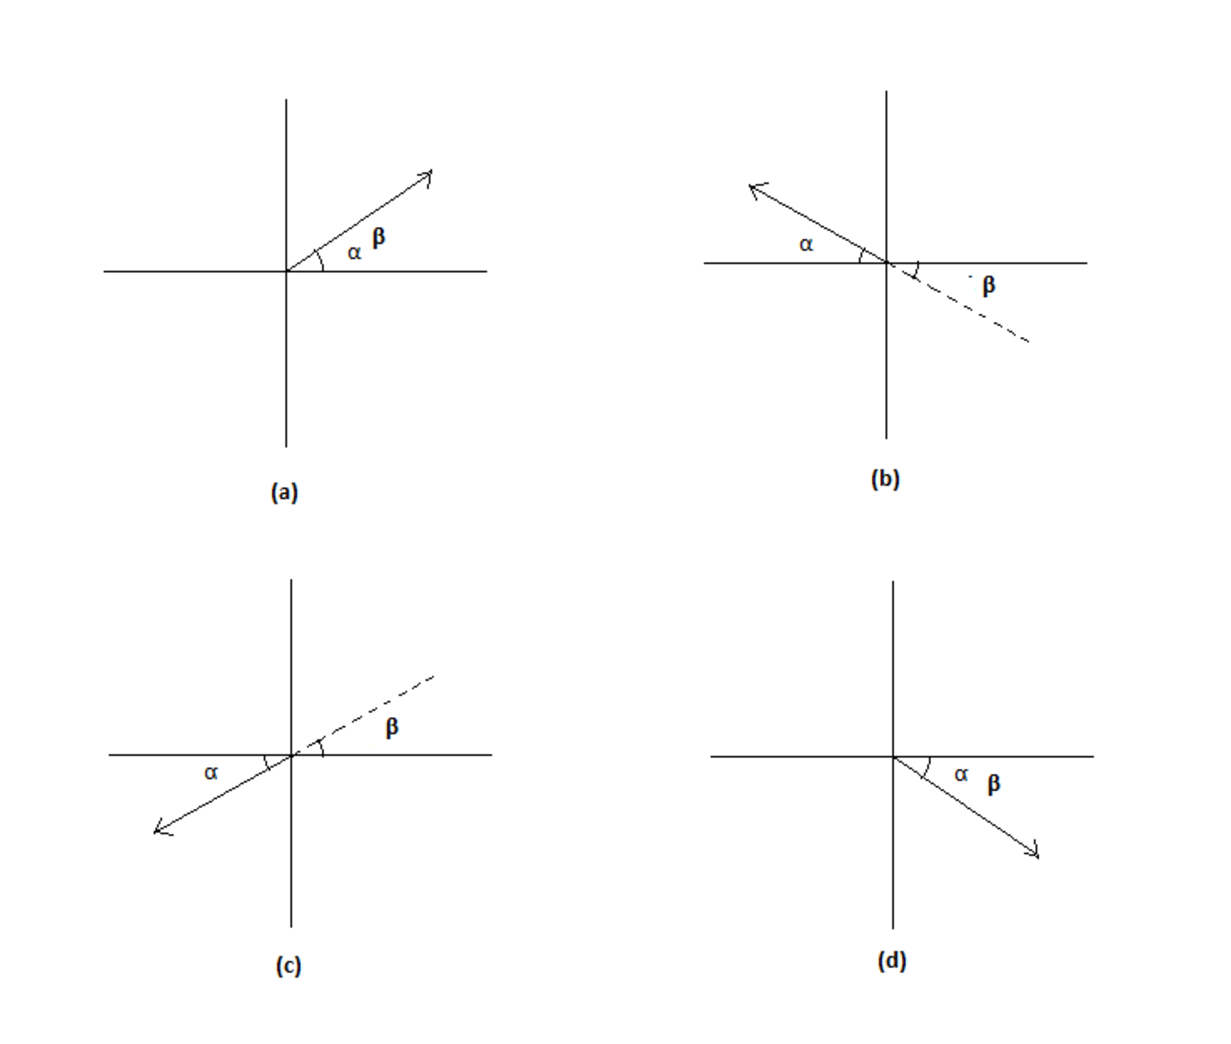
\includegraphics[width=0.48\textwidth]{atan.eps}
%   \end{center}
%   \caption{Angle value returned by gcc compiler}
%     \label{Fig:gcc}
% \end{wrapfigure}
%  
% The function atan() in GCC returns a value between $\frac{-\pi}{2}$ and $\frac{\pi}{2}$ as shown in Figure \ref{Fig:gcc}. The slope, $\frac{N_y}{N_x}$ of normal to interface
% is given as input to atan$\left(\frac{N_y}{N_x}\right)$ return the value of the acute angle made by the x-axis. 
% The returned value is positive when in first and third quadrant and negative when in second and fourth quadrant. 
% To make it positive the fabs function is used.
% \begin{eqnarray*}
% \beta = atan\left(\frac{N_y}{N_x}\right), 
% \qquad \alpha =\lvert\beta\lvert 
% \end{eqnarray*}
% 
% Hence, the expression for GCC to calculate theta becomes
% 
\begin{equation}
 \theta=\frac{\pi}{2}-fabs\left(atan\left(\frac{N_x}{N_y}\right)\right)
 \end{equation}
%  Note: Every step after calculating $\theta$, will have first reorient the normal to the first quadrant.
% The code treats all the quadrants as the first quadrant after suitable rotation.
 
\subsubsection{Step V: Shape Identification}
There are four possible shapes in a 2D reconstruction 
If the volume fraction and $\theta$ is fixed then the shape is decided as in Figure \ref{Fig:shape_region}. The various regions are identified as follows.
\begin{figure}
 \centering
    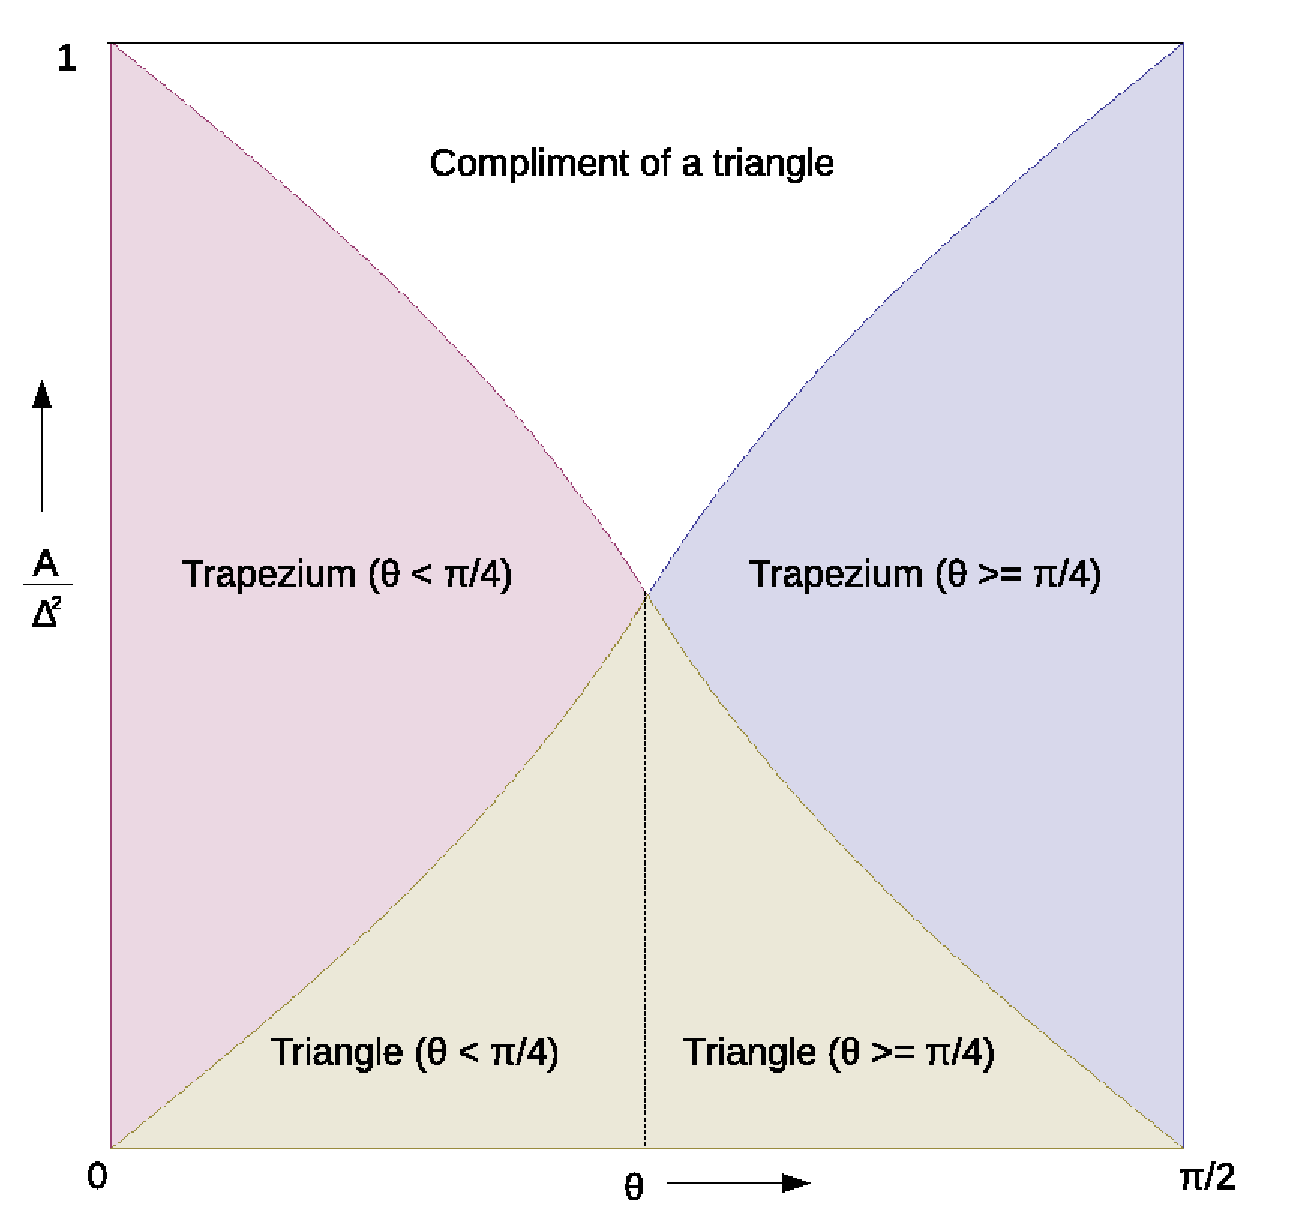
\includegraphics[scale=0.5]{shape_region.eps}
  \caption{Area and angle region}
  \label{Fig:shape_region}
\end{figure}
\underline{Triangle}\\
Area of fluid, $A=\Delta^2F$ 

From Figure \ref{Fig:triangle}, we get,

\begin{figure}%[H] 
\centering
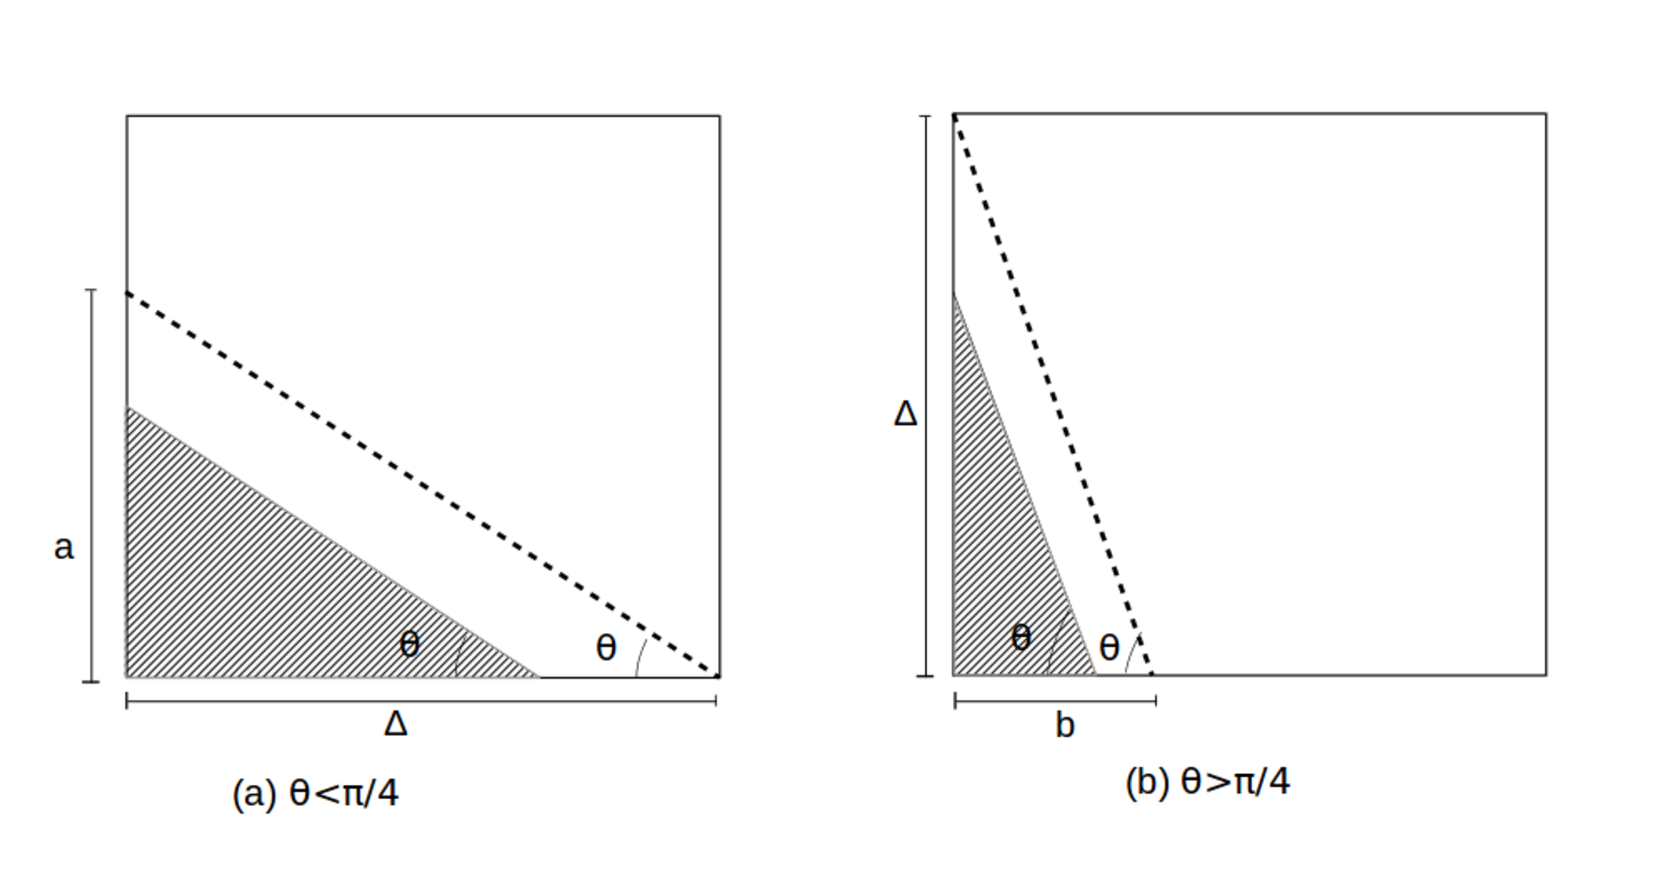
\includegraphics[scale=0.4]{triangle.eps}
\caption{Area of the triangle made by dark fluid in the cell}
\label{Fig:triangle}
\end{figure}

\begin{eqnarray*}
 a&=&\Delta tan\theta \text{\quad $\theta < \frac{\pi}{4}$} \\  
 b&=&\frac{\Delta}{tan\theta} \text{\quad $\theta >= \frac{\pi}{4}$}\\
\end{eqnarray*}

\begin{equation*}
\boxed{\begin{align}
    \frac{A}{\Delta^2} <= \frac{1}{2} tan\theta \qquad \text{for, }\theta < \frac{\pi}{4} \\
    \frac{A}{\Delta^2}<=  \frac{1}{2tan\theta} \qquad \text{for, }\theta > \frac{\pi}{4}   
    \end{align}}
\end{equation*}

\underline{}{For trapezium},\\

\begin{figure}%[H]
\centering
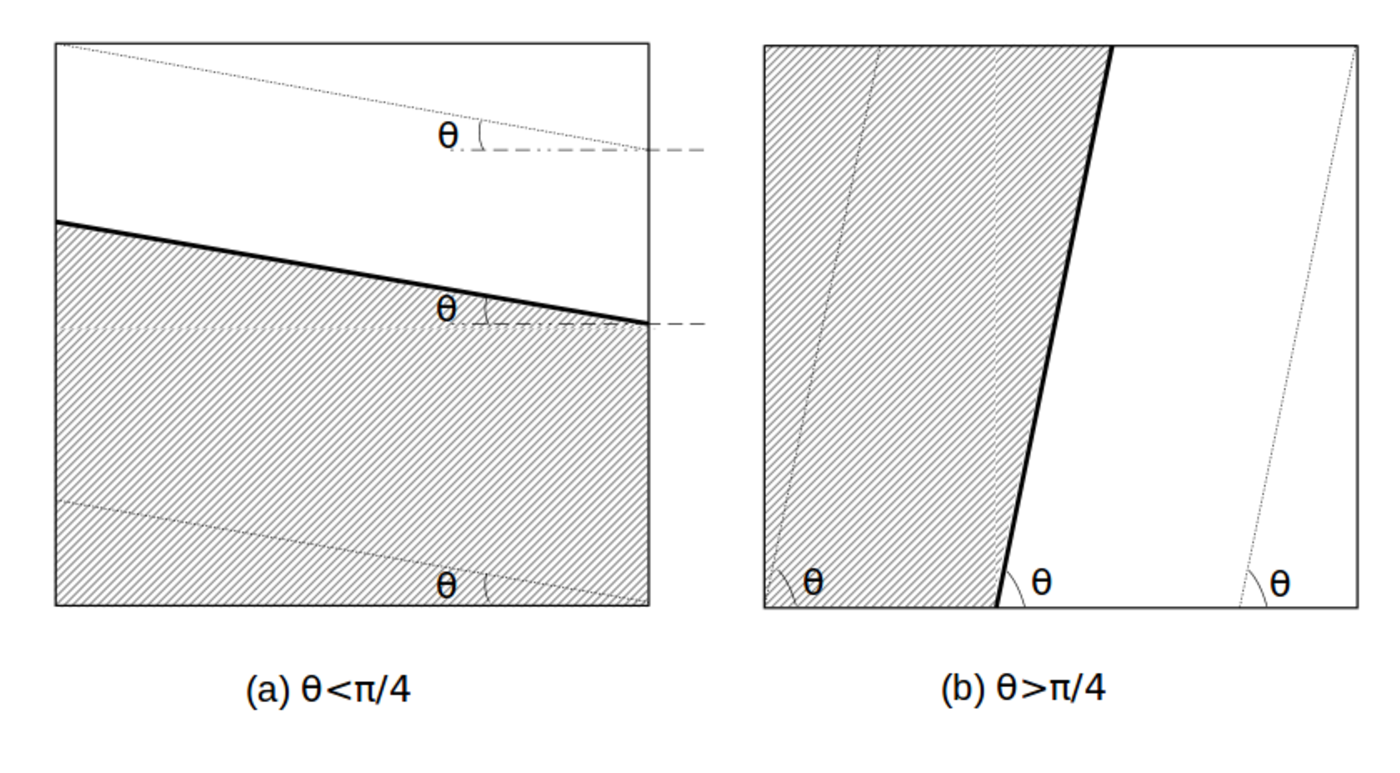
\includegraphics[scale=0.4]{trapezium.eps}
\caption{Area of a trapezium made by the dark fluid in the cell}
\end{figure}

\begin{figure}
 \centering
 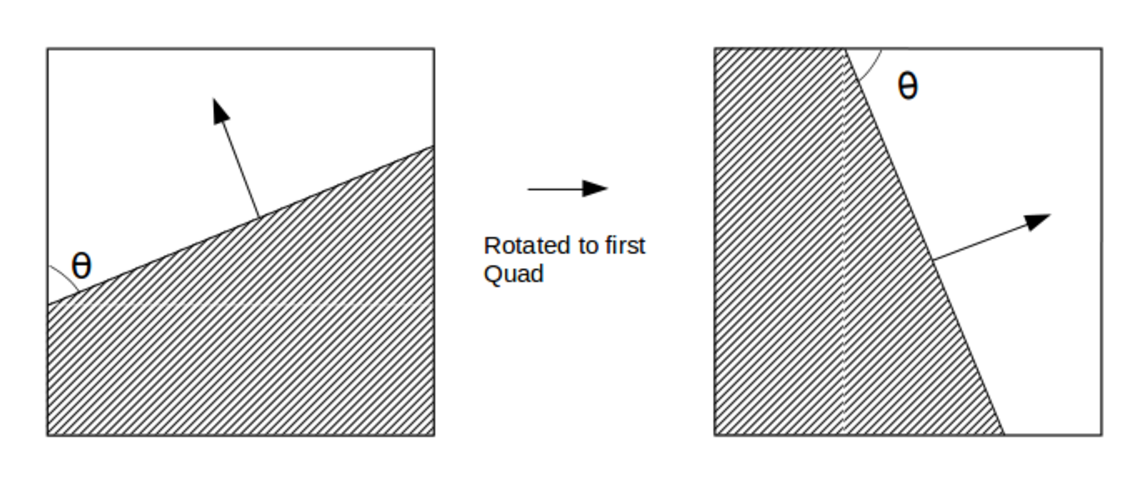
\includegraphics[scale=0.6]{2ndQuad.eps}
 \caption{When the cell is reoriented to make normal lie in first quadrant}
 \label{Fig:reorientation}
\end{figure}

In Figure \ref{Fig:reorientation}, it can be seen that when the cell reoriented to make the normal in first quadrant the $\theta$ becomes the angle with the horizontal axis.
Hence, the same calculations can be applied to this cell for what is done for first quadrant. 

\begin{equation*}
\boxed { \begin{align}
 \frac{1}{2} tan\theta <& \frac{A}{\Delta^2}< \left(1-\frac{1}{2} tan\theta\right)  \qquad \text{for, } \theta < \frac{\pi}{4} \nonumber	\\    
   \frac{1}{2tan\theta} <&   \frac{A}{\Delta^2}< \left(1-\frac{1}{2tan\theta}\right) \qquad \text{for, }  \theta >= \frac{\pi}{4}	
   \end{align}}
\end{equation*}
For all other cases the shape becomes a compliment of a triangle.

\subsubsection{Step VI: Perpendicular distance Calculation }
After reorientation, the perpendicular distance will now be always from the LHS corner of the cell.\\
\underline{Triangle}\\
Note the following formulae for Figure \ref{Fig:trianlge_p}

\begin{eqnarray*}
c=\frac{b}{cos\theta},
\qquad b=\frac{p}{sin\theta},  
\qquad  c=\frac{p}{sin\theta cos\theta},
\qquad   \frac{1}{2}pc=F\Delta^2,
\qquad  \frac{p^2}{sin2\theta}=F\Delta^2 \nonumber
\end{eqnarray*}

\begin{equation*}
\boxed{ \begin{align}
  p=\sqrt{F\Delta^2sin2\theta}
  \end{align} }
\end{equation*}
  
\begin{figure}
\centering
 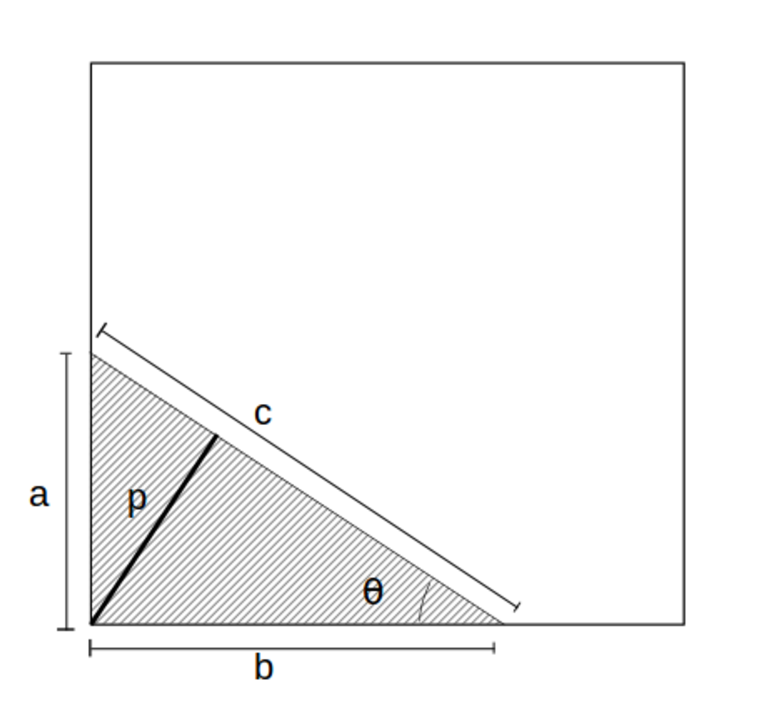
\includegraphics[scale=0.4]{triangle_p.eps}
 \caption{Perpendicular distance in a triangle}
 \label{Fig:trianlge_p}
\end{figure}

\underline{Trapezium}, \\
  \begin{figure}
  \centering
    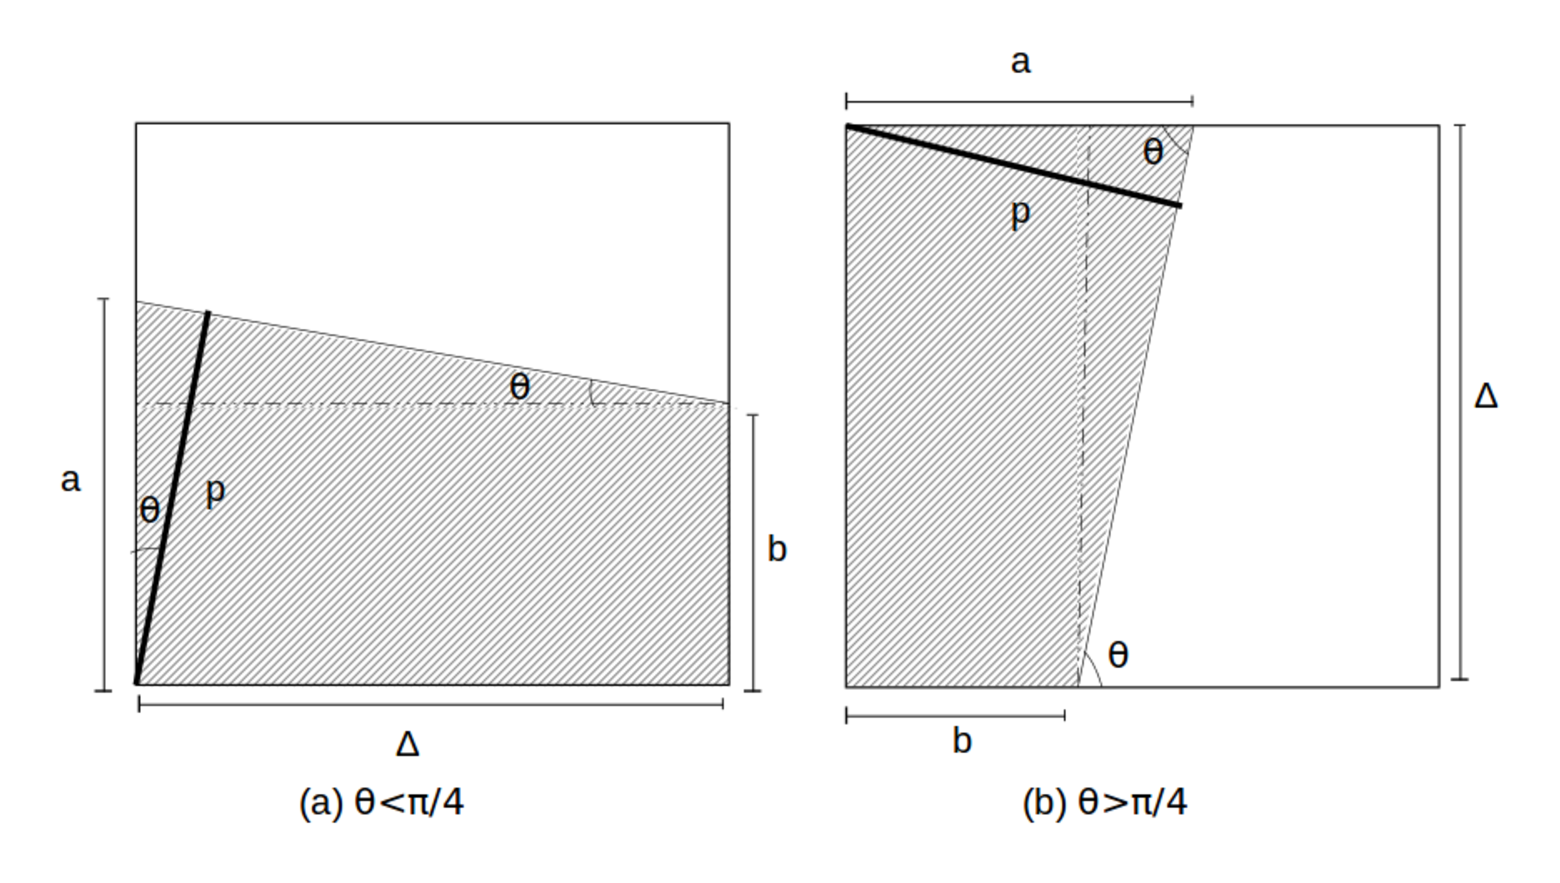
\includegraphics[scale=0.4]{trapezium_p.eps}
    \caption{Perpendicular distance for a trapezium}
    \label{Fig:trapezium_p}
  \end{figure}
  Note the formulae for Figure \ref{Fig:trapezium_p}
  
  \begin{equation*}
  \begin{aligned}  
     \text{For} \quad \theta  < \frac{\pi}{4}, 
    \qquad  \Delta^2 F &=\frac{(a+b)\Delta}{2},
    \qquad a=\frac{p}{cos\theta},
      \qquad tan\theta=\frac{a-b}{\Delta},
      \qquad b=\frac{p}{cos\theta}-\Delta tan\theta, \\
      \\
      \text{or,}\qquad \frac{1}{2}\Delta\left(\frac{2p}{cos\theta}-\Delta tan\theta\right)&=\Delta^2 F,
      \qquad \boxed{p=\Delta Fcos\theta+\frac{1}{2}\Delta sin\theta} \\
      \\
\text{For} \quad \theta  >= \frac{\pi}{4},
\qquad
\Delta^2 F &=\frac{(a+b)\Delta}{2}
\qquad
a=\frac{p}{sin\theta},
\qquad
tan\theta=\frac{\Delta}{a-b},
\qquad
b=\frac{p}{sin\theta}-\frac{\Delta}{tan\theta},\\
\\
\text{or,}\qquad 0.5\Delta\left(\frac{2p}{sin\theta}-\frac{\Delta}{tan\theta}\right)&=\Delta^2 F,
\qquad
\boxed{p=\Delta Fsin\theta+\frac{1}{2}\Delta cos\theta}
\end{aligned}
  \end{equation*}
  
\underline{For compliment of triangle},
\begin{figure}[H]
\centering
 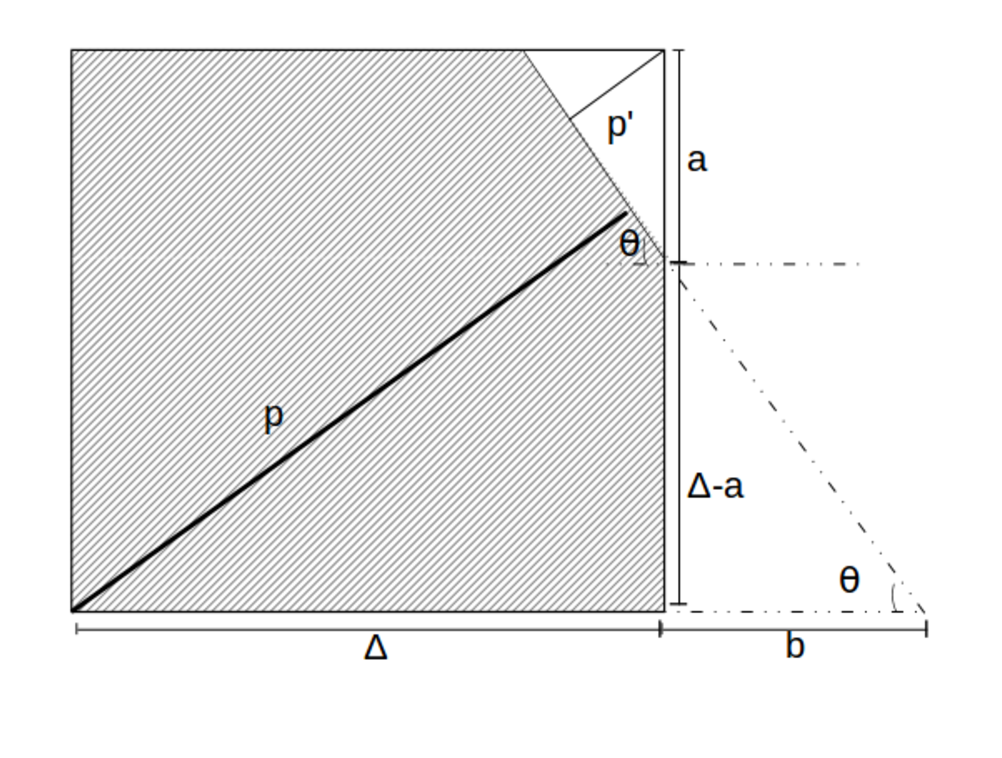
\includegraphics[scale=0.3]{compliment_p.eps}
 \caption{Perpendicular distance for compliment of the triangle}
\end{figure}

\begin{equation*}
\begin{align}
 p'&=&\sqrt{F\Delta^2sin2\theta},
\qquad a=\frac{p'}{cos\theta},\\
\\
\text{or,}\qquad b&=&\frac{\Delta-a}{tan\theta},
\qquad \boxed{p=\Delta(sin\theta+cos\theta)-p'}
\end{align}
\end{equation*}

\subsubsection{Step VII : Line Extrapolation}
After, reorientation of the line to the first quadrant. A line can be constructed with the $\theta$ and perpendicular distance using normal form, (See Figure \ref{Fig:normal})
\begin{figure}
 \centering
 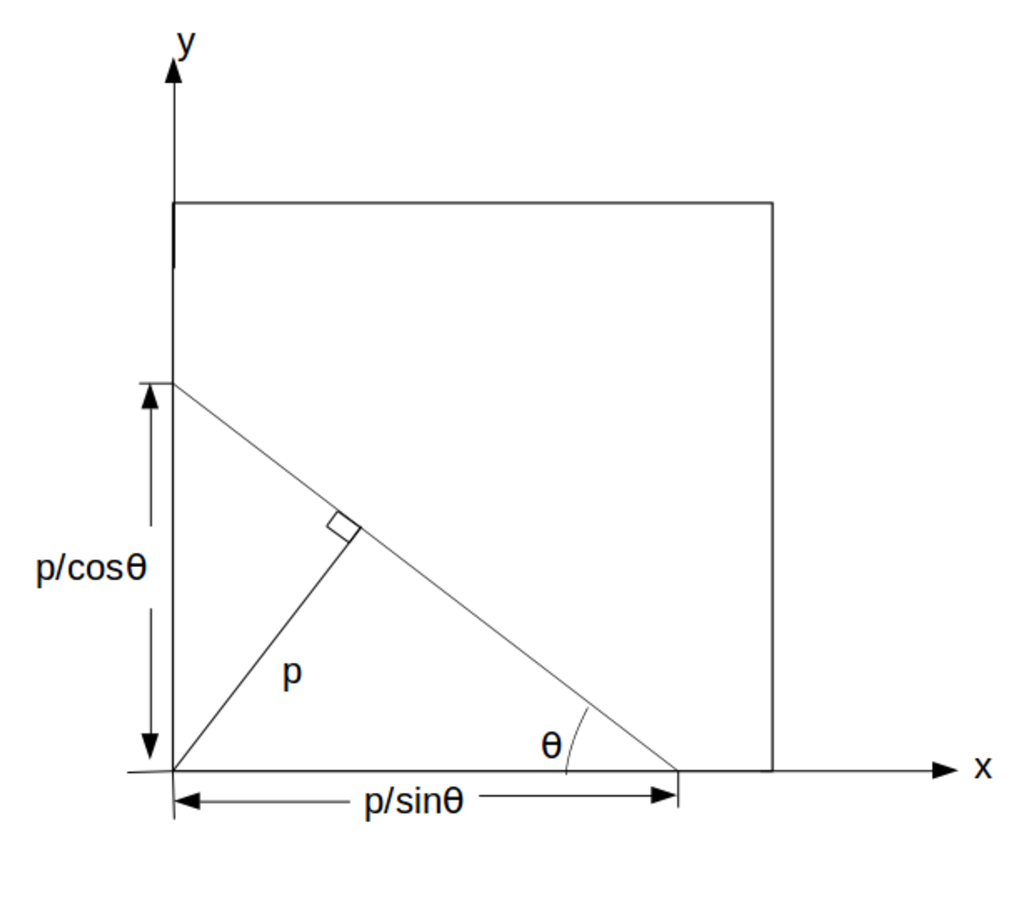
\includegraphics[scale=0.4]{normal_form.eps}
 \caption{Normal form of a line in the cell}
 \label{Fig:normal}
\end{figure}
\begin{equation}
 x\sin\theta+y\cos\theta = p
\end{equation}

Refer to Figure \ref{Fig:extrapolation} for extrapolation,

\begin{figure}%[H]
 \centering
 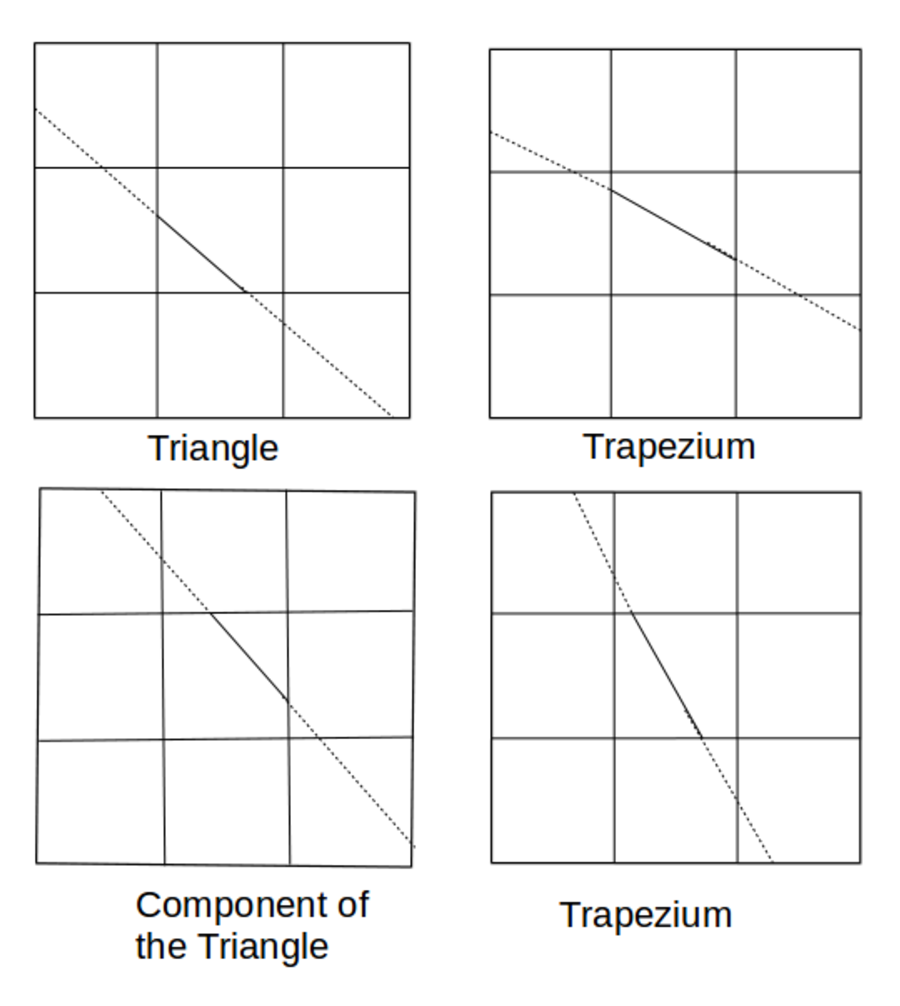
\includegraphics[scale=0.4]{extrapolate.eps}
 \caption{Extrapolation of the line in 3 X 3 cell}
 \label{Fig:extrapolation}
\end{figure}

After extrapolation the new volume fraction is calculated under each cell below the line, which is then used to calculate the norm.
\subsubsection{Step VIII: Norm Calculation}
Let the new volume fraction calculated be $\widetilde F_{r,c}$. Now the norm which is here the difference of original volume fraction and new 
volume fraction calculated after the extrapolation are squared and then summed over 3 X 3 stencil. Also, called as $L^2$ norm, \\
\begin{equation*}
 \boxed{L^2(\theta) =  \sum_{k,l=-1}^{1}(\widetilde F_{r+k,c+l}-F_{r+k,c+l})^2}
\end{equation*}

\subsubsection{Step IX : Norm Minimization}
After calculating norm the initial guess of slope and $\theta$ is changed with small step size but it should not be confused with rotation of interface or normal.
All the steps are repeated to after modifying theta and norm is again calculated. This process repeats when a minima of norm reached. And the final values of $\theta$,
shape, and quadrant are assigned to the cell.

\subsection{Advection}
The Equation \ref{Eq:advection_vof} is also solved using geometrical technique by calculating fluxes across the cells and then updating the F-field in each time step. Direct finite differencing
of this equation will lose the discontinuous property of F-field and cause smearing of interface as shown in Figure \ref{Fig:smearing}\\
% 
\underline{Flux Calculation}\\
% The flux is calculated through the wall of the cells in X an Y directions.
% for first quadrant all cases are discussed below, for all other quadrants reorientation of normal works,
% For X-Flux when velocity in x-direction, u is positive then only the right wall of the left cell will affect the flux (See Figure 11)
The flux of fluid through the walls is calculated using a graphical technique. A typical cell is shown in Figure \ref{Fig:triangle_t} and the through its right wall is calculated .
Various possibilities arise and these are discussed below.
\subsubsection{\underline{Triangle}}
For a triangle there are two cases:-\\
if $(\Delta-udt)>x_0$, Nothing will leave from the right wall \\
if $(\Delta-udt)<x_0$, A triangle leaves. \\
here $x_0$ is the value of x at $y=0$.
\begin{figure}%[H]
 \centering
 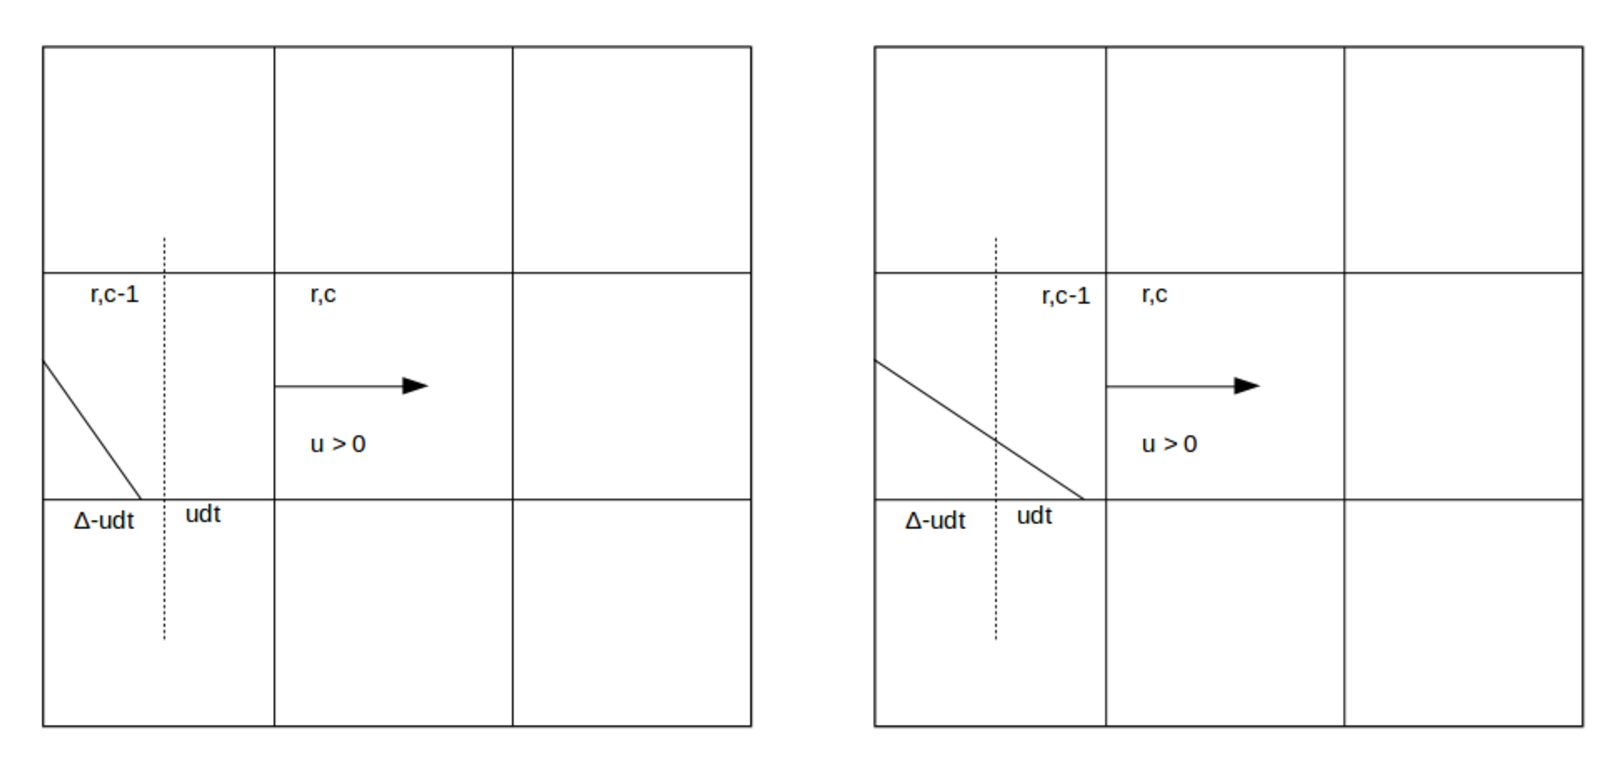
\includegraphics[scale=0.4]{ad_triangle.eps}
 \caption{Cases for a triangle in flux calculation}
 \label{Fig:triangle_t}
\end{figure}
The area of this triangle is given by,
\begin{equation*}
 \boxed{Flux = \frac{1}{2}(x_0 - \Delta + udt)^2 \tan\theta}
\end{equation*}

\subsubsection{\underline{Trapezium}}
Two types of trapezium can be in the first quadrant, $\theta<\frac{\pi}{4}$, and $\theta>\frac{\pi}{4}$, \\
(See Figure \ref{Fig:trapezium} and \ref{Fig:trapezium_cases}) \\
\begin{figure}%[H]
\centering
 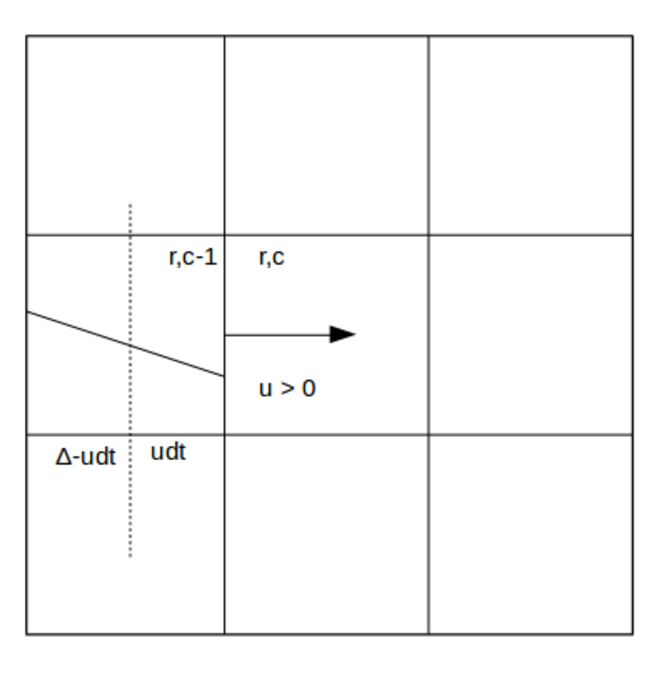
\includegraphics[scale=0.4]{ad_trapezium.eps}
 \caption{Flux calculation for trapezium for $\theta<\frac{\pi}{4}$}
 \label{Fig:trapezium}
\end{figure}

\begin{figure}%[H]
 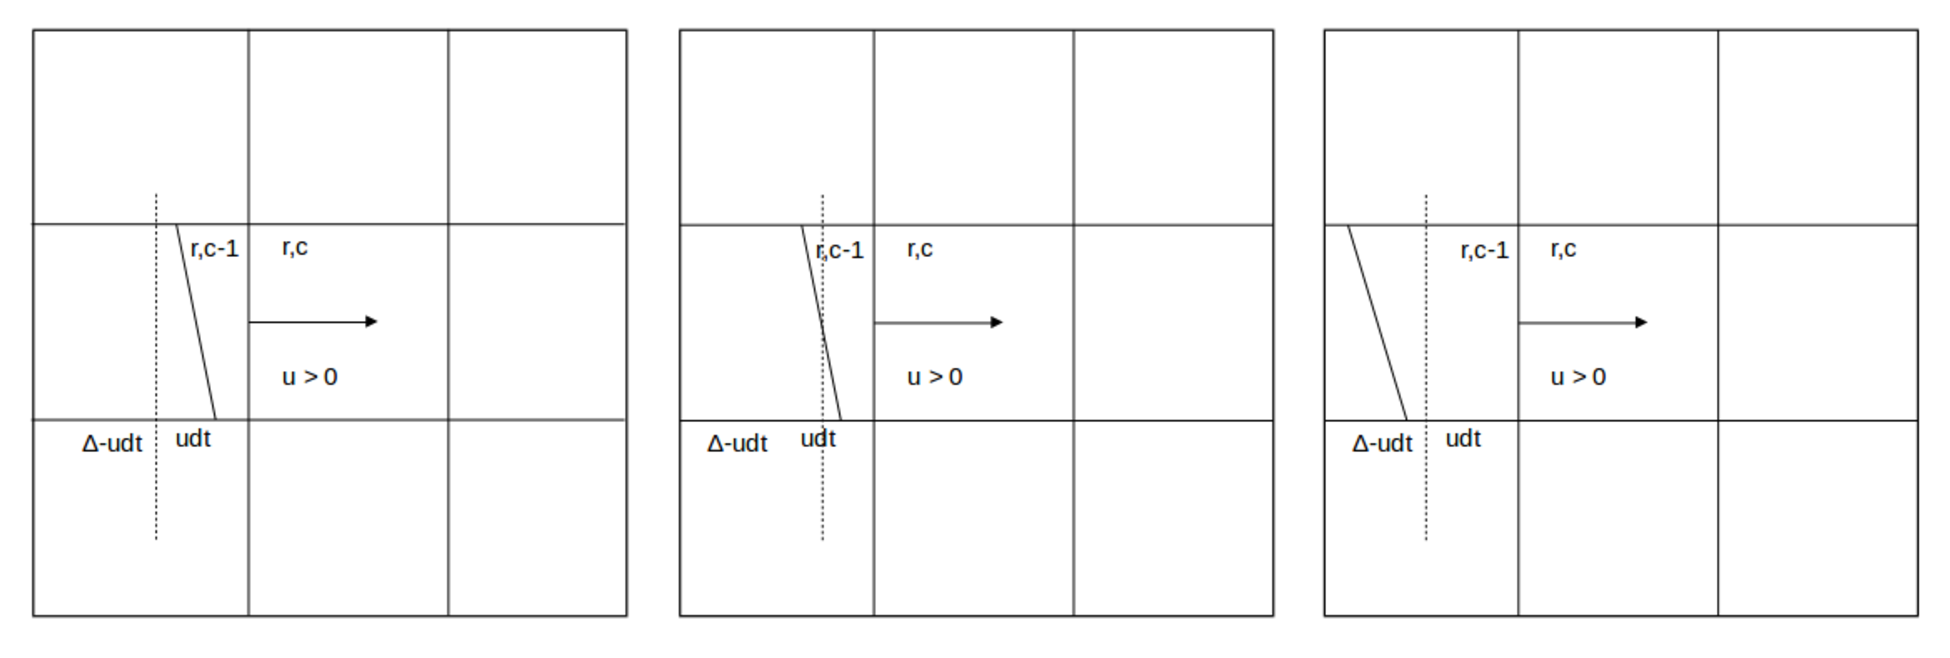
\includegraphics[scale=0.4]{ad_trap_pi4.eps}
 \caption[Different cases for flux calculation for trapezium]{(a)$(\Delta-udt)<x_{del}$, (b)$x_{del}<=(\Delta-udt)<x_0$, (c)$(\Delta-udt)>=x_0$}
 \label{Fig:trapezium_cases}
\end{figure}

For $\theta<\frac{\pi}{4}$, the only possibility is that a trapezium leaves and its area is given by,
\begin{eqnarray*}
 Flux = \frac{1}{2}( y_0 - ((\Delta - udt) \tan\theta) + y_{del} ) udt \\
\end{eqnarray*}

\begin{equation*}
 \begin{align}
 &\text{For } \theta>\frac{\pi}{4}, \\
 \text{For } &(\Delta-udt)<x_{del},  \text{ a trapezium leaves the cell and the Flux is given by,} \\
&\boxed{ Flux = \frac{\Delta}{2}(x_{del} - (2(\Delta - udt)) + x_0) }\\
 \text{For }  &x_{del}<=(\Delta-udt)<x_0,  \text{ a triangle leaves the cell and the flux is given by,} \\
&\boxed{Flux =\frac{1}{2\tan\theta} (y_0 - (\Delta - udt)\tan\theta))^2} \\
\text{For } & ((\Delta-udt))>=x_0,  \text{nothing leaves from the cell.} \\
&\boxed{Flux =0}
\end{align}
\end{equation*}

\subsubsection{\underline{Compliment of a triangle}}
For compliment of a triangle two cases arise, (See Figure \ref{Fig:compliment_triangle})
\begin{figure}%[H]
 \centering
 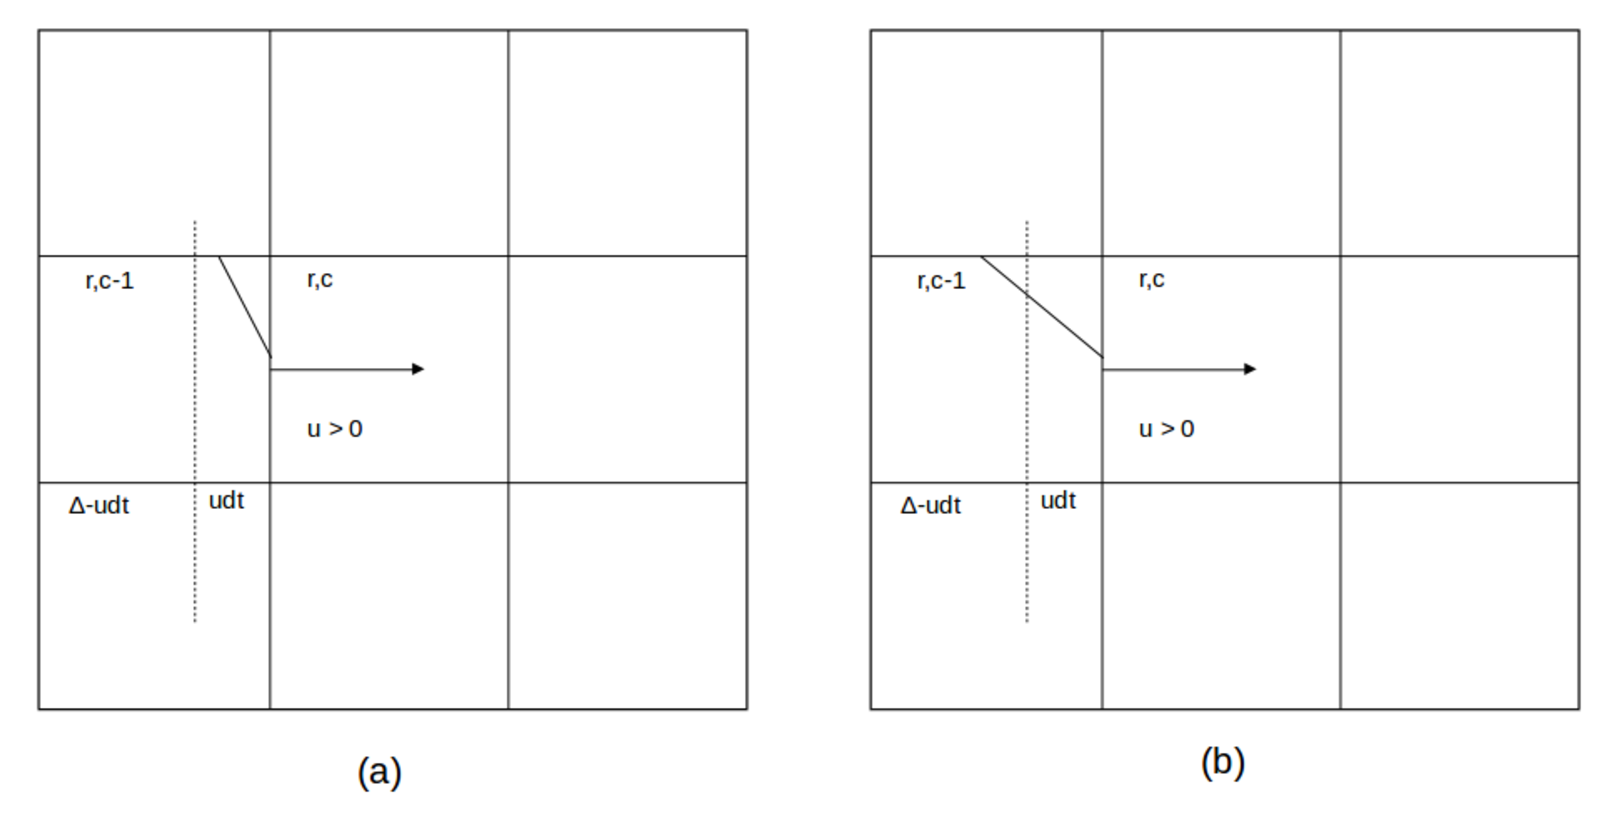
\includegraphics[scale=0.4]{ad_comp.eps}
 \caption[Different cases for flux calculation for compliment of a triangle]{(a)$(\Delta-udt) < x_{del}$, (b)$(\Delta-udt) >= x_{del}$}
 \label{Fig:compliment_triangle}
\end{figure}
\begin{equation*}
\begin{aligned}
\text{if, } \Delta -udt &< x_{del}, \text{ A 5-Sided figure leaves,  and Flux is given by,} \\
&\boxed{Flux = \Delta(x_{del} - \Delta + udt)) + \frac{1}{2}((\Delta + y_{del})(\Delta - x_{del}))} \text{ (sum of rectangle and trapezium)} \\
\text{if, } \Delta -udt &>= x_{del},  \text{ A trapezium leaves, and Flux is given by,} \\
&\boxed{Flux =  \frac{udt}{2}( y_{del} + y_0 - (\Delta - udt)\tan\theta)}
\end{aligned}
\end{equation*}

\subsection{Volume Fraction Calculation}
The fluxes calculated in the previous section are used to update the volume fractions in the cells for the next time step. For this we use \textit{Direction Split Young's method} (DSY).
\cite{Youngs1982}. In this method the order of directions is interchanged after each time step in order to avoid systematic errors. To achieve mass conservation, for this the 
basic condition is velocity divergence. In this method, the mass cannot be conserved until all directions are taken into consideration. Hence the values of volume fraction larger than unity
and less than zero may arise after first sweep which violates the restriction, $0\leqslant F\geqslant=1$ for the next sweep. This difficulty can be solved by introducing effective 
volume of the cells (\cite{Rudman1997}). But this induces risks of small under- or overshoots. Undershoot occurs when the all the volume fraction has to be fluxed out from the cell 
but it does not and cell cannot be emptied, overshoot occurs when the cell in fluxed with the volume fraction to get filled but it does not. Both occurs because of use of effective volume
in calculation of fluxes through wall. This can be resolved by using flux correction in the second sweep \cite{Lorstad2004}. The following algorithm is used to calculate the volume 
fractions for the 2D flow. \\
Effective volume(non-dimensional, characteristic area $\Delta^2$) for the $I^{st}$ sweep,
\begin{equation*}
 \delta V^I_{r,c} = 1 - \Delta t \frac{V_{out}-V_{in}}{\Delta} 
\end{equation*}
where, $\delta V^I_{r,c}$ is the effective volume after $I^{st}$ sweep. \\
Net Flux out $\Delta J_{out}$, (non-dimensional) in or out in a cell is given by,
\begin{equation*}
 \Delta J_{out} = \frac{(J_{out}-J_{in})}{\Delta^2} 
\end{equation*}

From which Volume Fraction after $I^{st}$ of the cell is given by,
\begin{equation*}
\boxed{F_{r,c}^I =  \frac{F^0 - \Delta J_{out}}{\delta V^1_{r,c}}}
\end{equation*}
where, $F^0$ and $F^I$ are the volume fractions before $I^{st}$ sweep and after $I^{st}$ sweep respectively.

For $II^{nd}$ sweep, 
\begin{equation*}
 \begin{align}
U^*_{out}  &= \frac{\Delta t}{\Delta}u_{out} \\
 \zeta &=
\begin{cases}
 \zeta_1 = \frac{J_{out}}{U^*_{out}} & \text{if} |\zeta_1-\frac{1}{2}| \geqslant  |\zeta_2-\frac{1}{2}| \\
\zeta_2 = \frac{F_{r,c}-J_{out}}{1-U^*_{out}} & \text{if} |\zeta_1-\frac{1}{2}| <  |\zeta_2-\frac{1}{2}| 
\end{cases} \\
\text{Corrected volume is given by,} \\
\delta V^{corr} &= F_{r,c} + (1-\delta V_{r,c}^I)\zeta \\
\text{Corrected outgoing flux is given by,} \\
J_{out}^{corr} &=  \delta V_{r,c}^I (J_{out}-U^*_{out}) + \delta V^{corr} U^*_{out} \\
\text{Corrected Total flux out from the cell is given by }\\
 \Delta J_{out}^{corr} &= J_{out}^{corr} - J_{in} \\
 \end{align}
 \end{equation*}
 \begin{equation*}
 \begin{align}
 \text{Final flux after last sweep is given by,}\\
 \boxed{F_{r,c}^{II} = F_{r,c}^{I} \delta V_{r,c}^I -  \Delta J_{out}^{corr}}
 \end{align}
\end{equation*}




\begin{figure}
 \subfloat[A circular interface\label{fig:1}]{%
      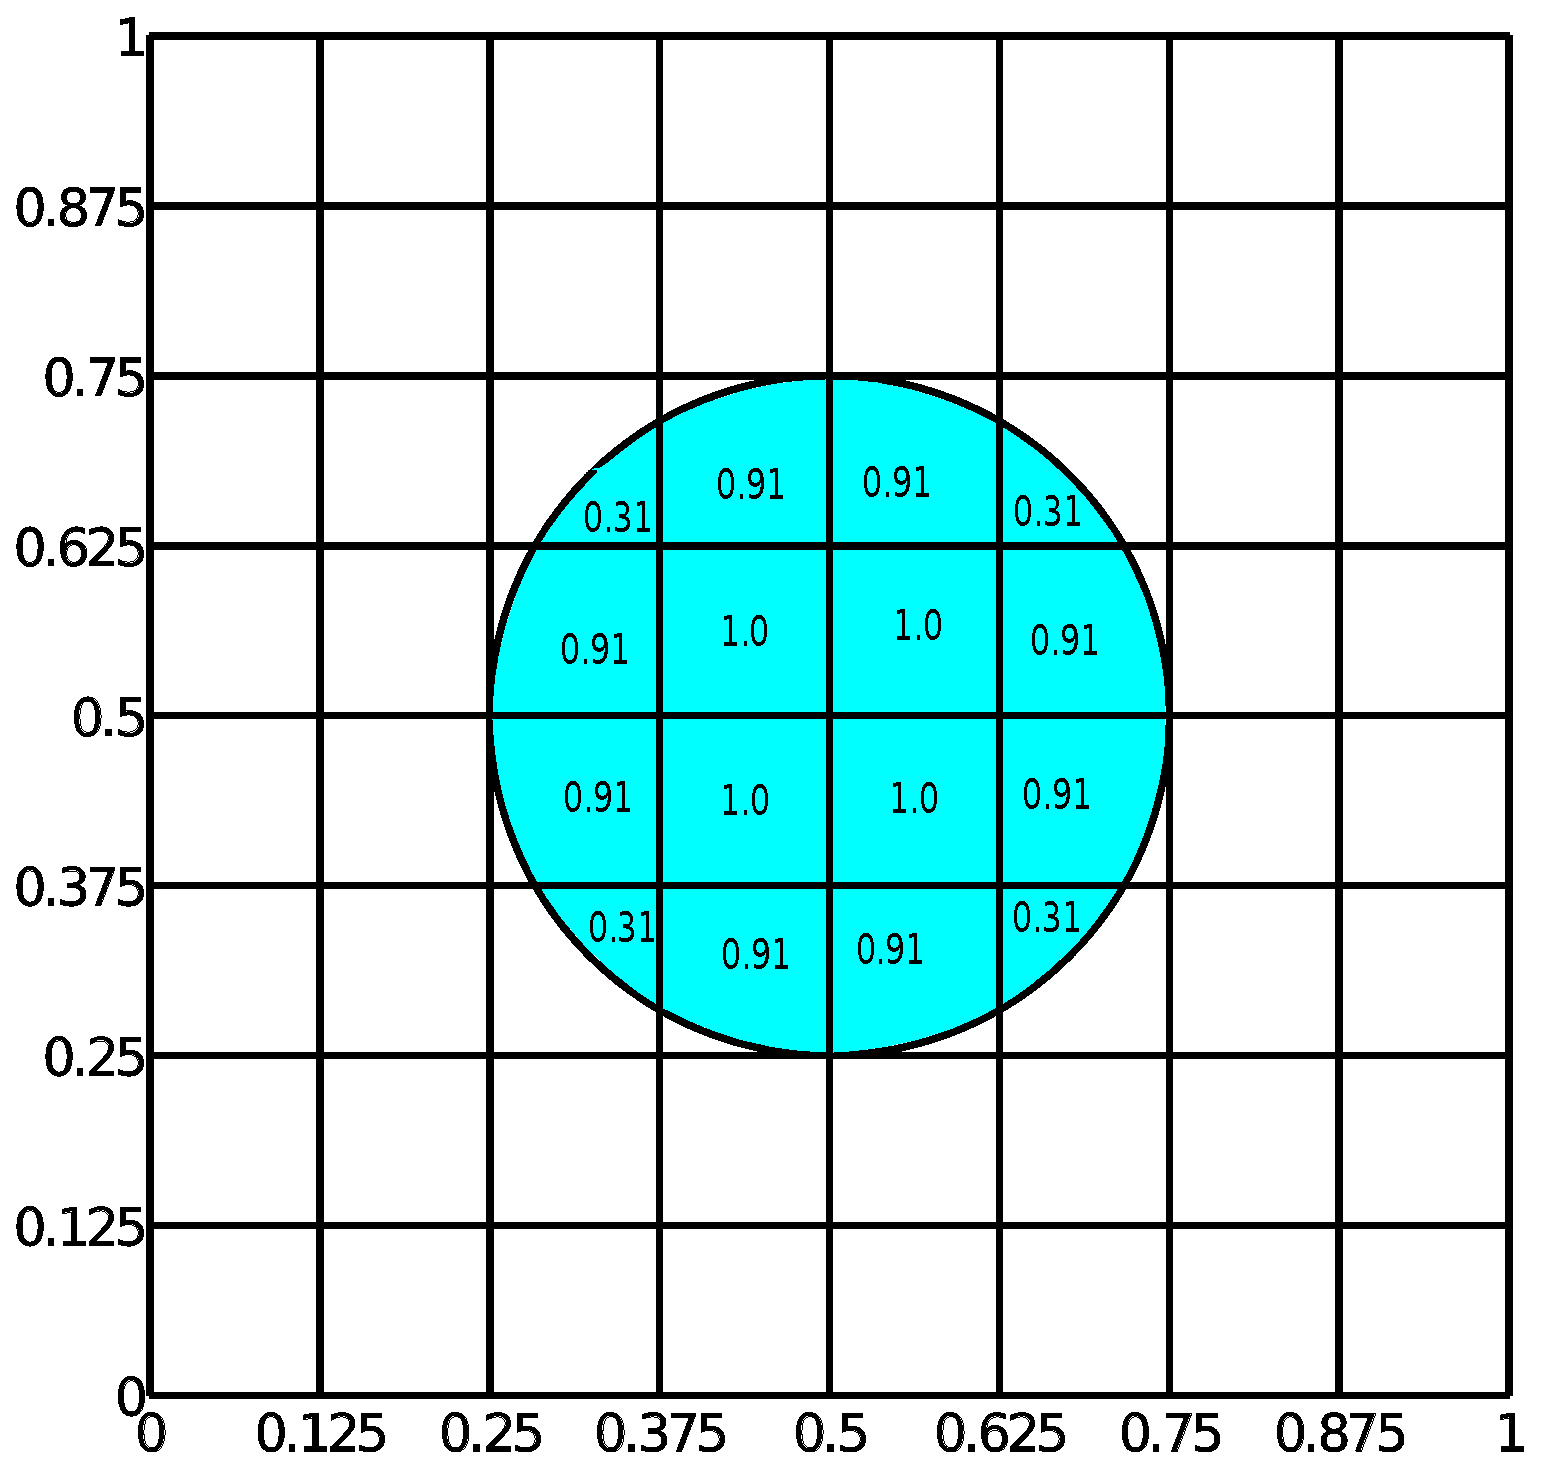
\includegraphics[width=0.5\textwidth]{circle_original_new.eps}
      }
  \subfloat[Reconstruction by LVIRA\label{fig:2}]{%
      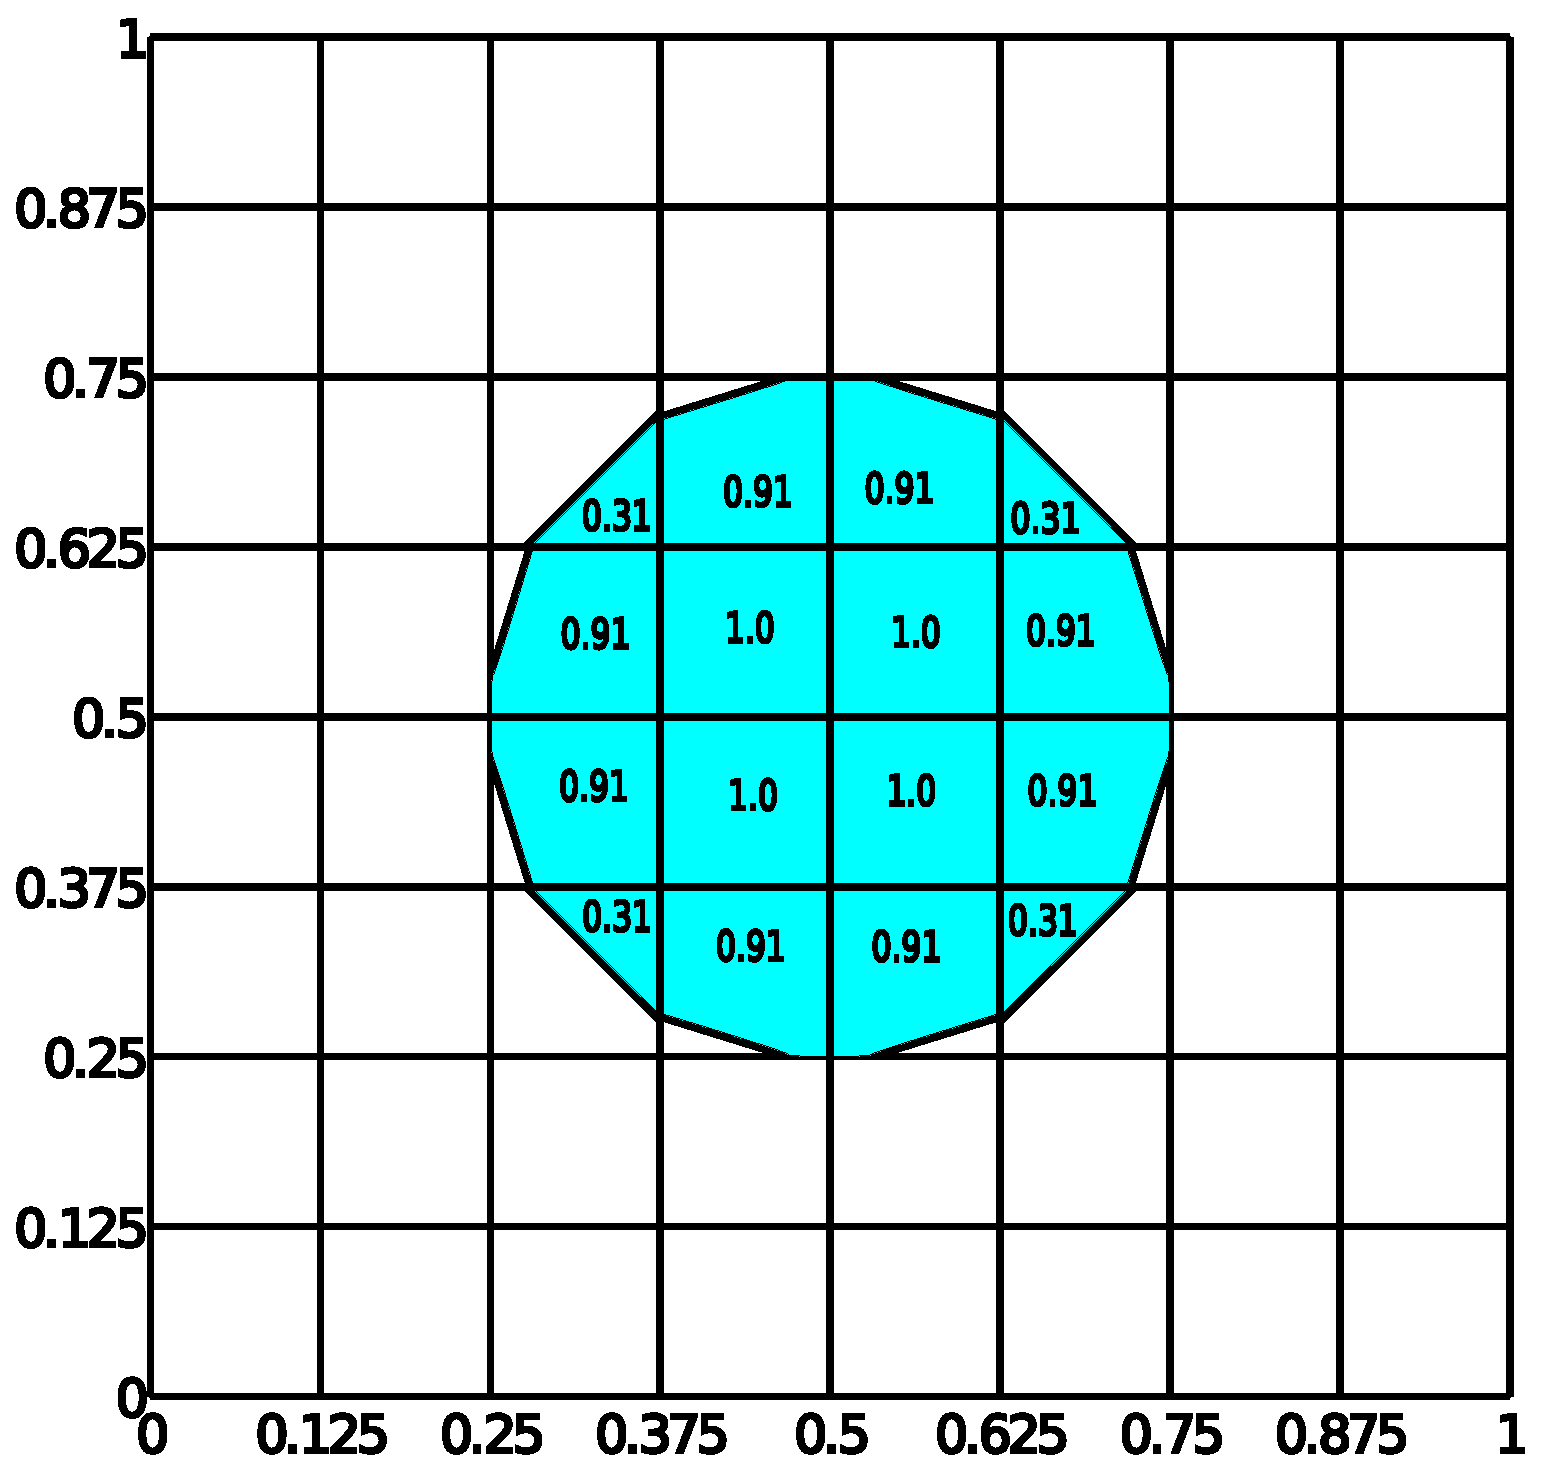
\includegraphics[width=0.5\textwidth]{circle_Recon_LVIRA.eps}
      }
 \caption{Reconstruction of a circular interface by LVIRA}
\end{figure}

\begin{figure}
 \subfloat[Flux calculation in x-direction\label{fig:3}]{%
      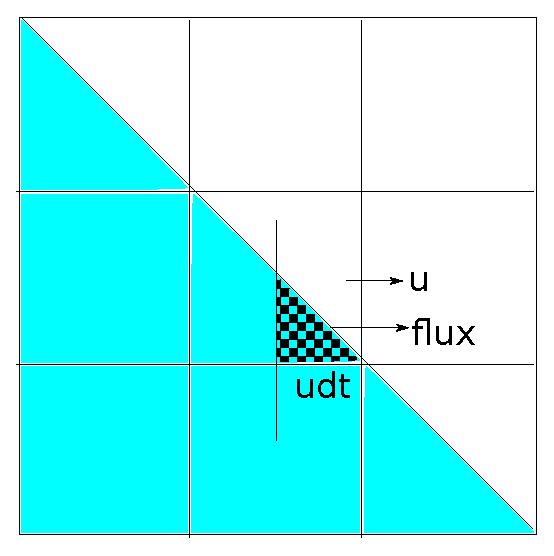
\includegraphics[width=0.5\textwidth]{u_ad.eps}
      }
  \subfloat[Flux calculation in x-direction\label{fig:4}]{%
      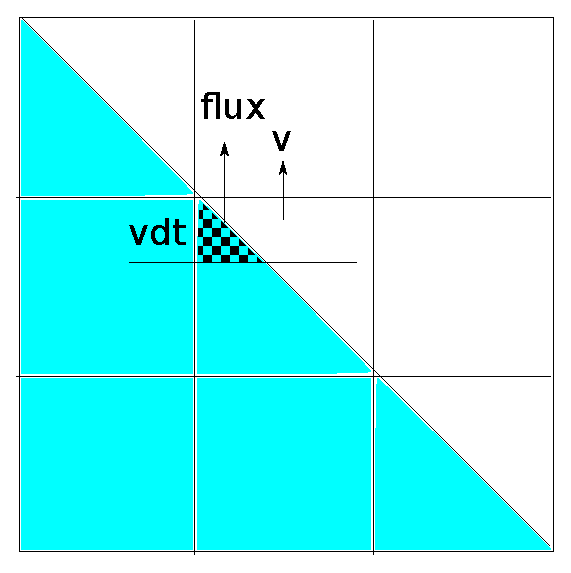
\includegraphics[width=0.5\textwidth]{v_ad.eps}
      }
 \caption{Advection of the interface by Youngs operator split algorithm}
\end{figure}

\section{Verification}
There are standard test cases are available in the literature: \cite{Zalesak1979}, \cite{Puckett1997}, \cite{Anton2001}, \cite{Gerlach2006} etc.
These involve advecting the interface with a fixed underlying velocity field of varying degree of complexity.
Volume of Fluid method is validated by choosing three test cases from \cite{Rudman1997}, 

\begin{enumerate}
 \item \textbf{Circle in translational flow} \\
 In this test the velocity field has zero velocity gradient and it is the simplest of all the tests.
 \item \textbf{Solid body rotation of slotted circle} \\
 The test has rate of strain tensor zero and gradient of velocity only has the vorticity component with constant angular velocity at every point in space.
 \item \textbf{Circle in shear flow} \\
Vorticity tensor in this test is zero and there is only the rate of strain tensor.
\end{enumerate}

\subsection{Advection of circle in translational flow}
The algorithm is tested for the simplest case of unidirectional velocity field. Two concentric circles are used as the initial 
condition for translational test, with center at (0.75,1) and diameter of inner and outer circle is 0.4 and 0.8 respectively (Figure \ref{Fig:translational_test}).
The volume fraction scalar field is advected by two velocity fields u=1,v=0 and u=2,v=1. The refinement of the domain which is [0,4] x [0,4] is 200 x 200. The time
step is 0.005 units and advection proceeds for 500 and 504 steps for case 1 and case 2 respectively.

\begin{figure}%[H]
 \centering
 \subfloat[Initial Condition for translational test]{%
      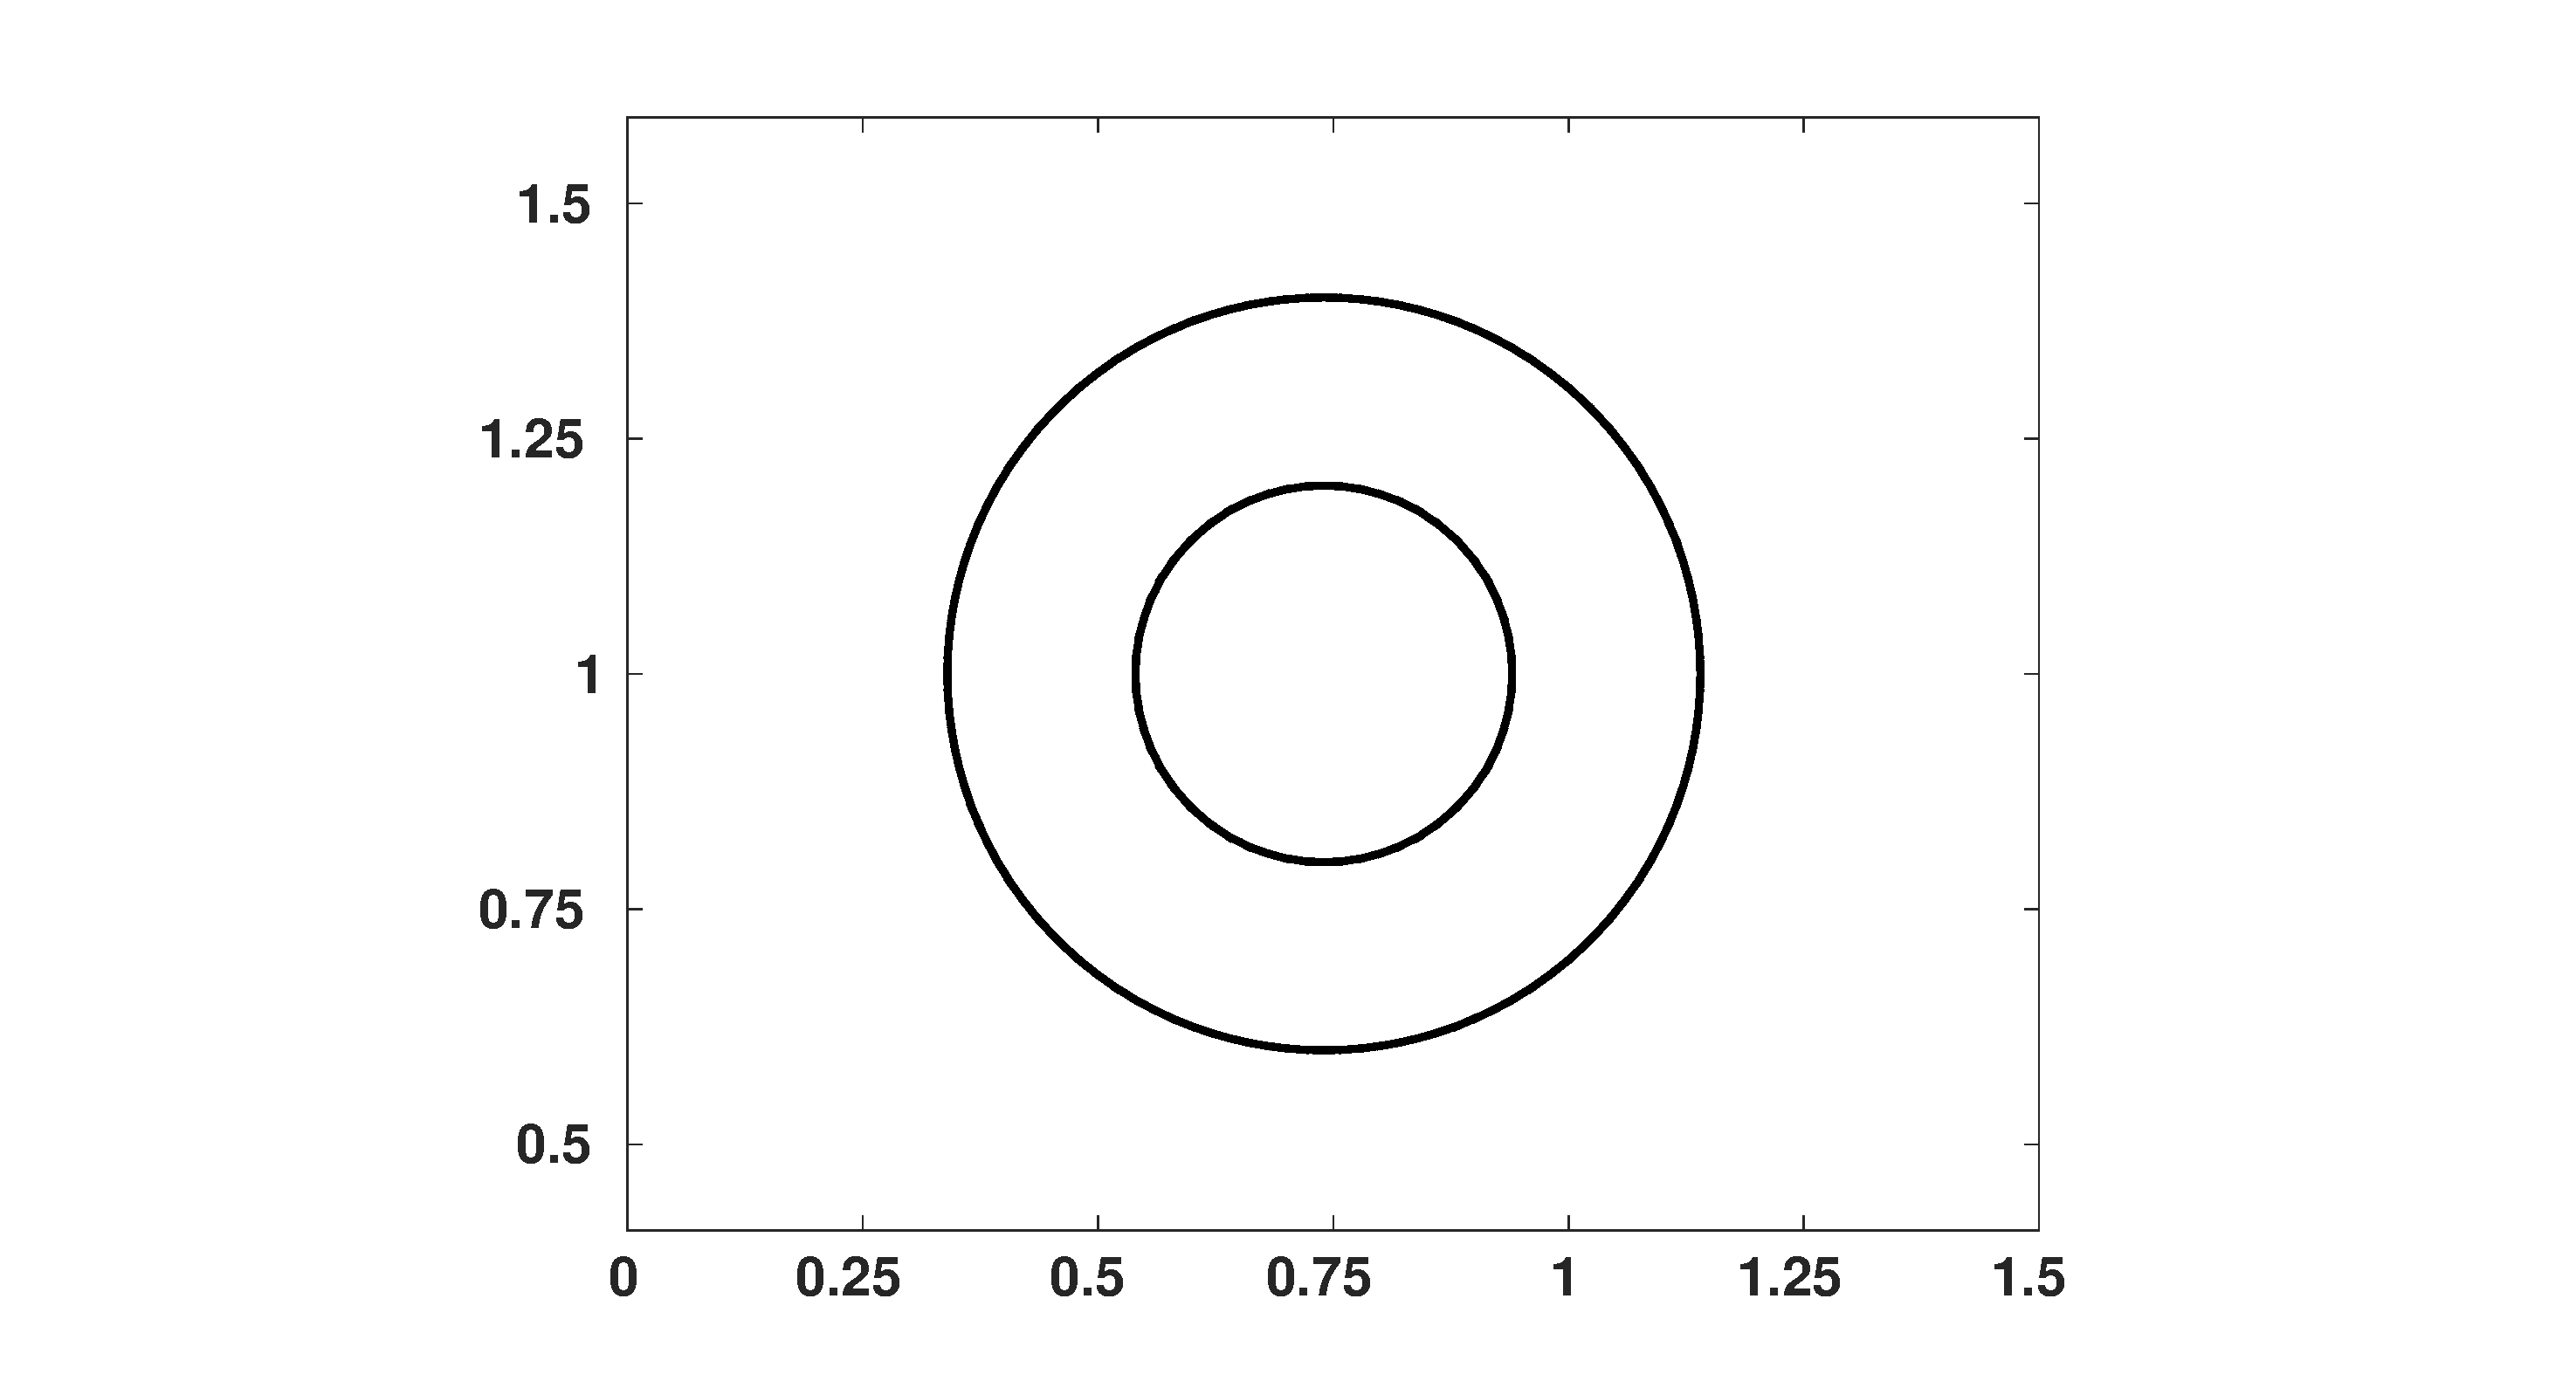
\includegraphics[width=0.5\textwidth]{IC.eps}
      }
  \subfloat[After advecting 500 steps ]{%
      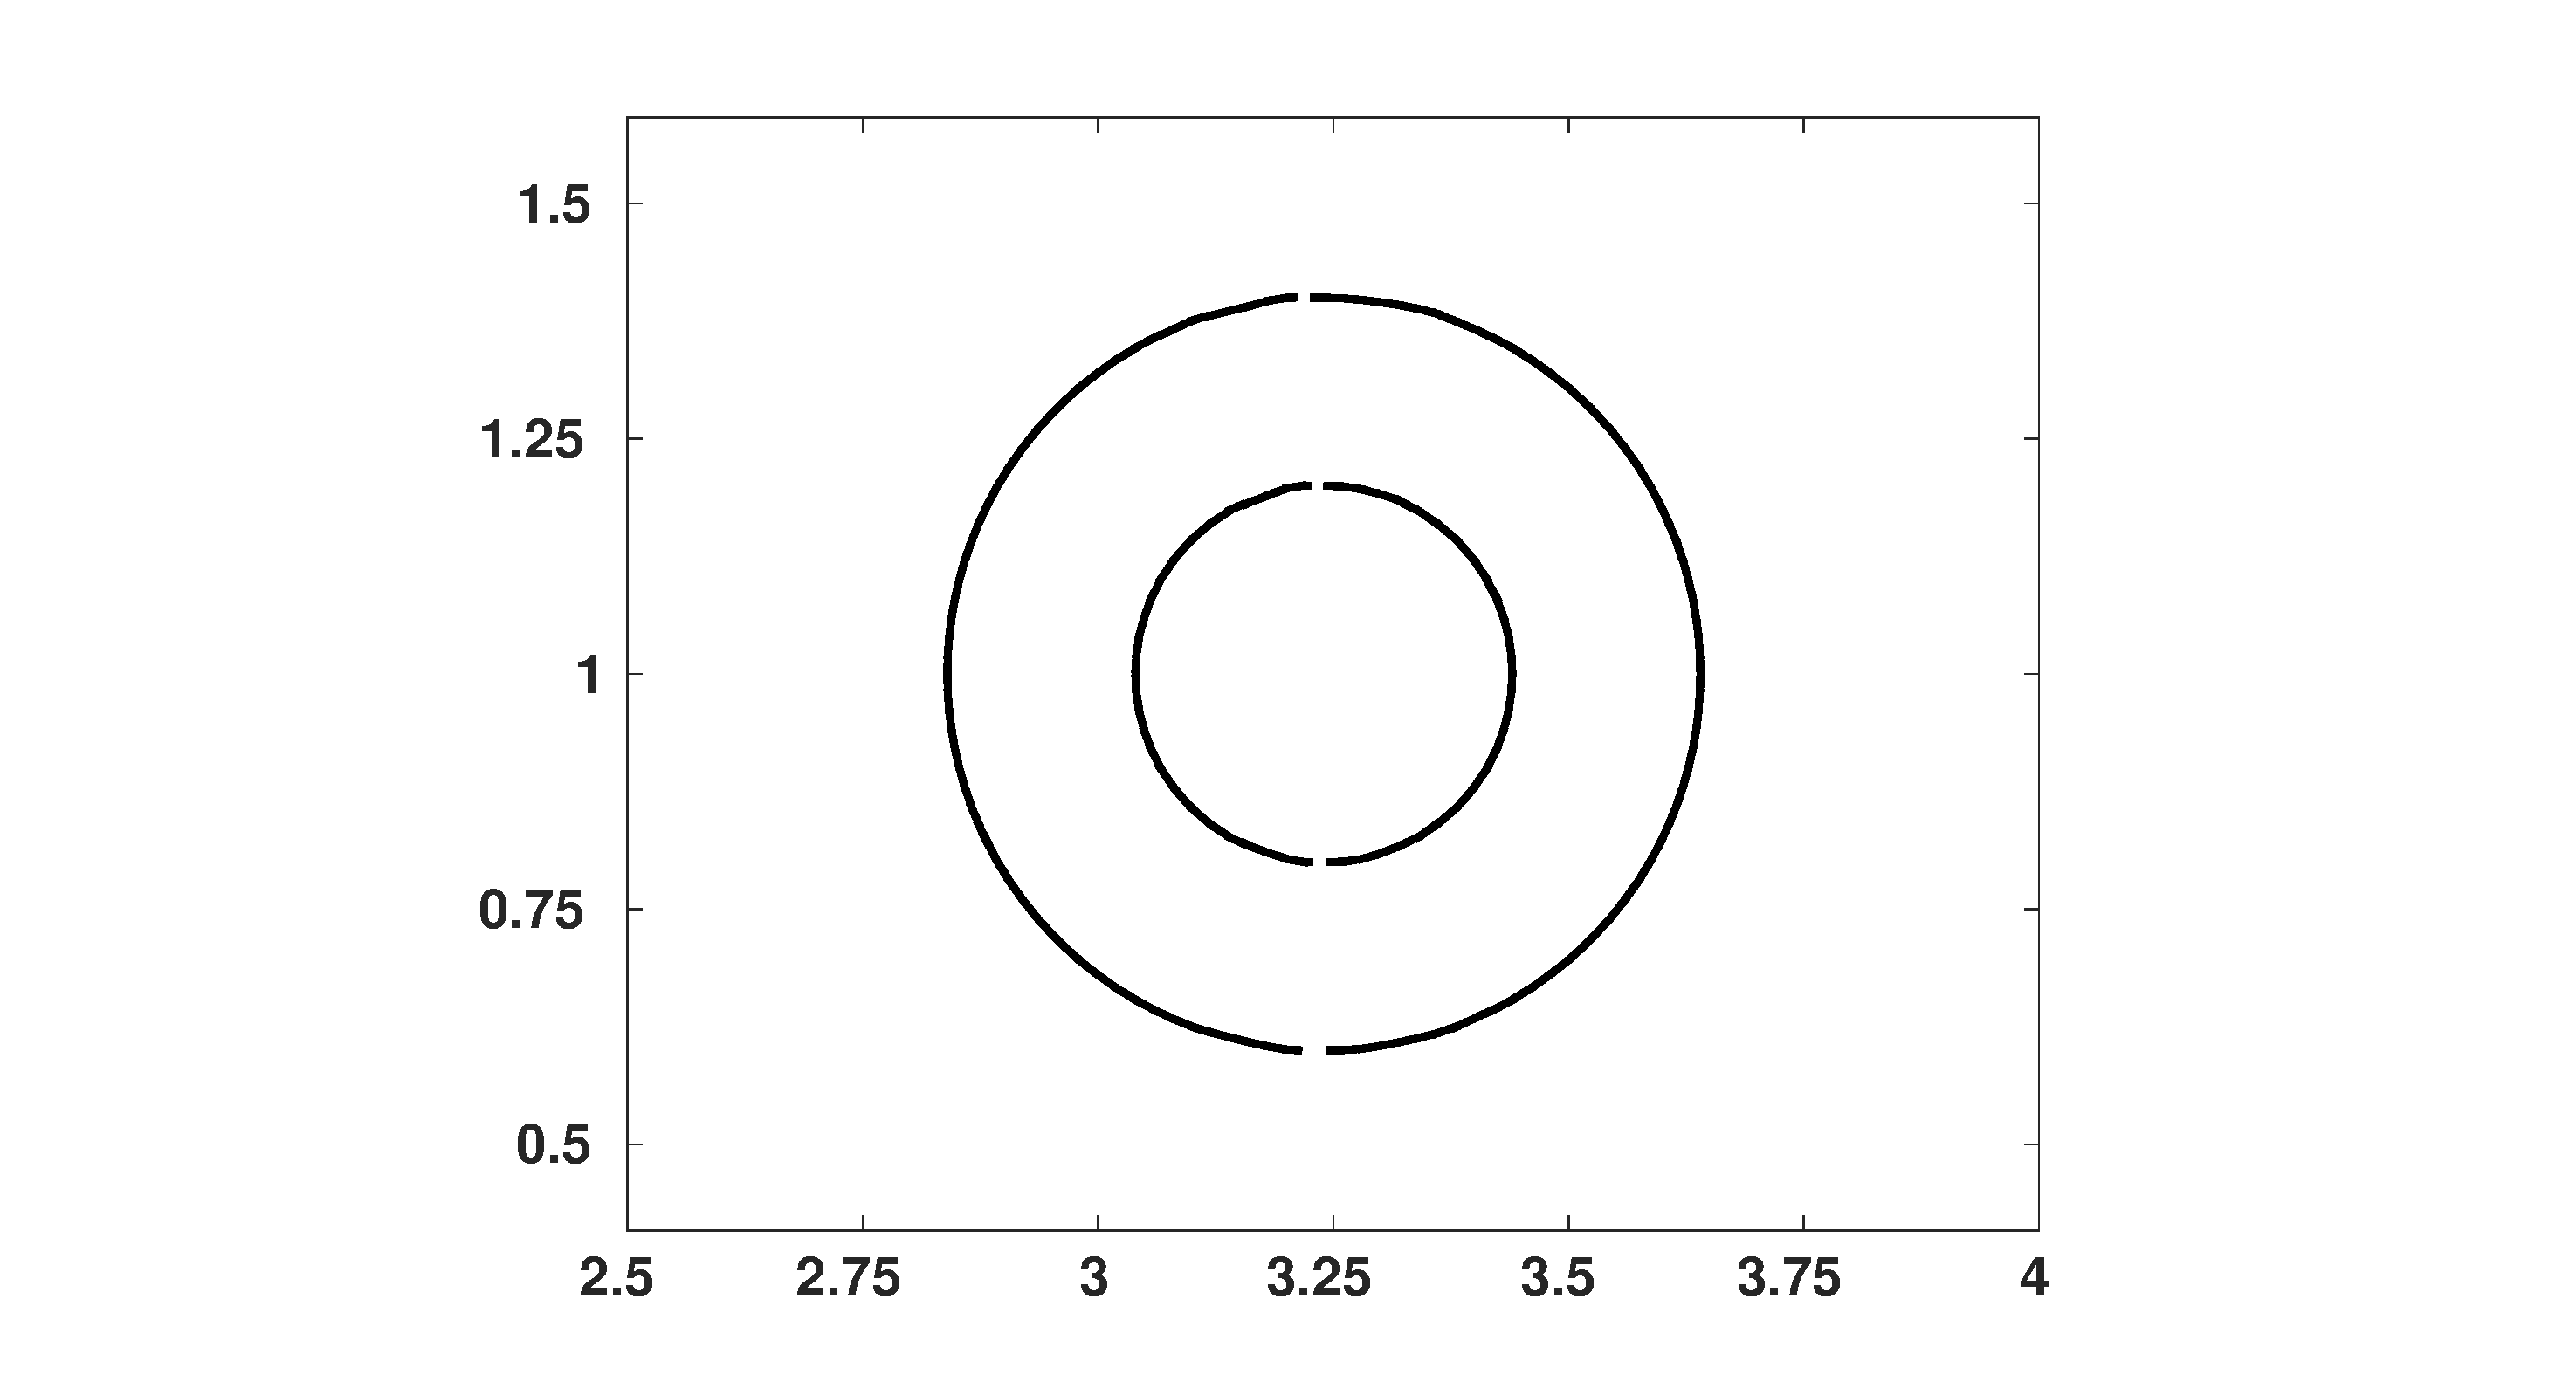
\includegraphics[width=0.5\textwidth]{final500.eps}
      }
 \caption{Advection test for velocity field u=1,v=0}
 \label{Fig:translational_test}
\end{figure}

\begin{figure}%[H]
 \centering
 \subfloat[Initial Condition for translational test ]{%
      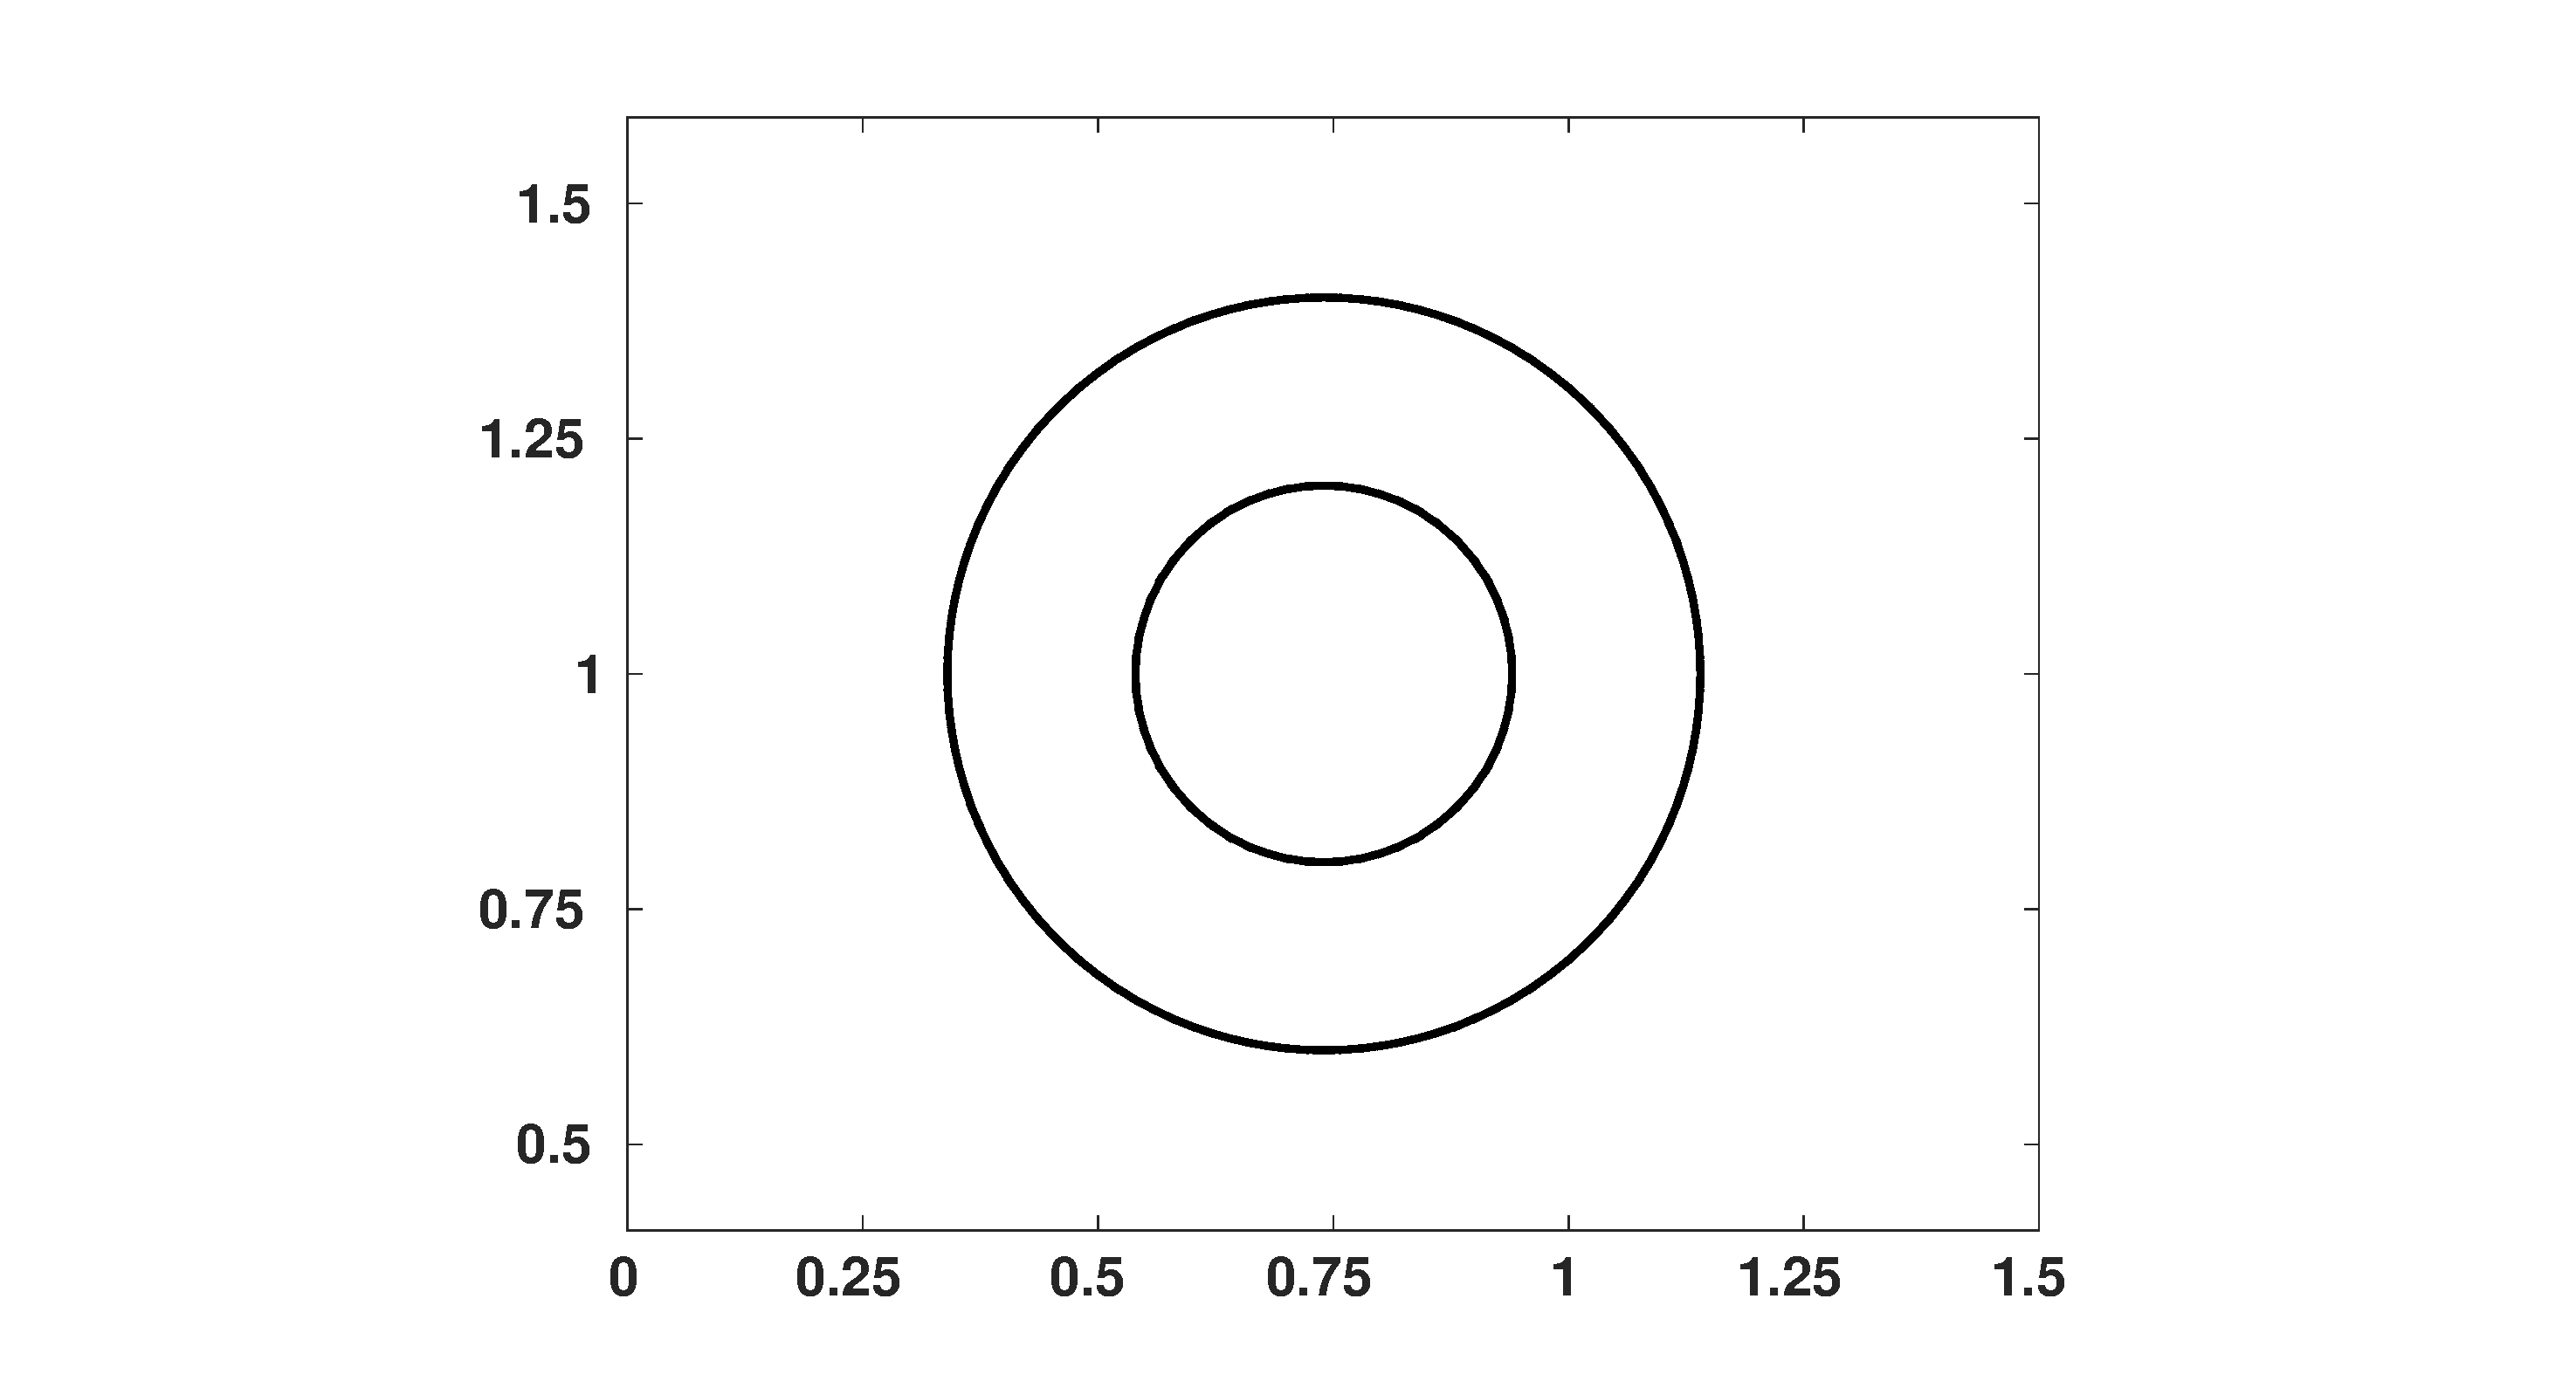
\includegraphics[width=0.5\textwidth]{IC21.eps}
      }
\subfloat[After advecting 504 steps ]{%
      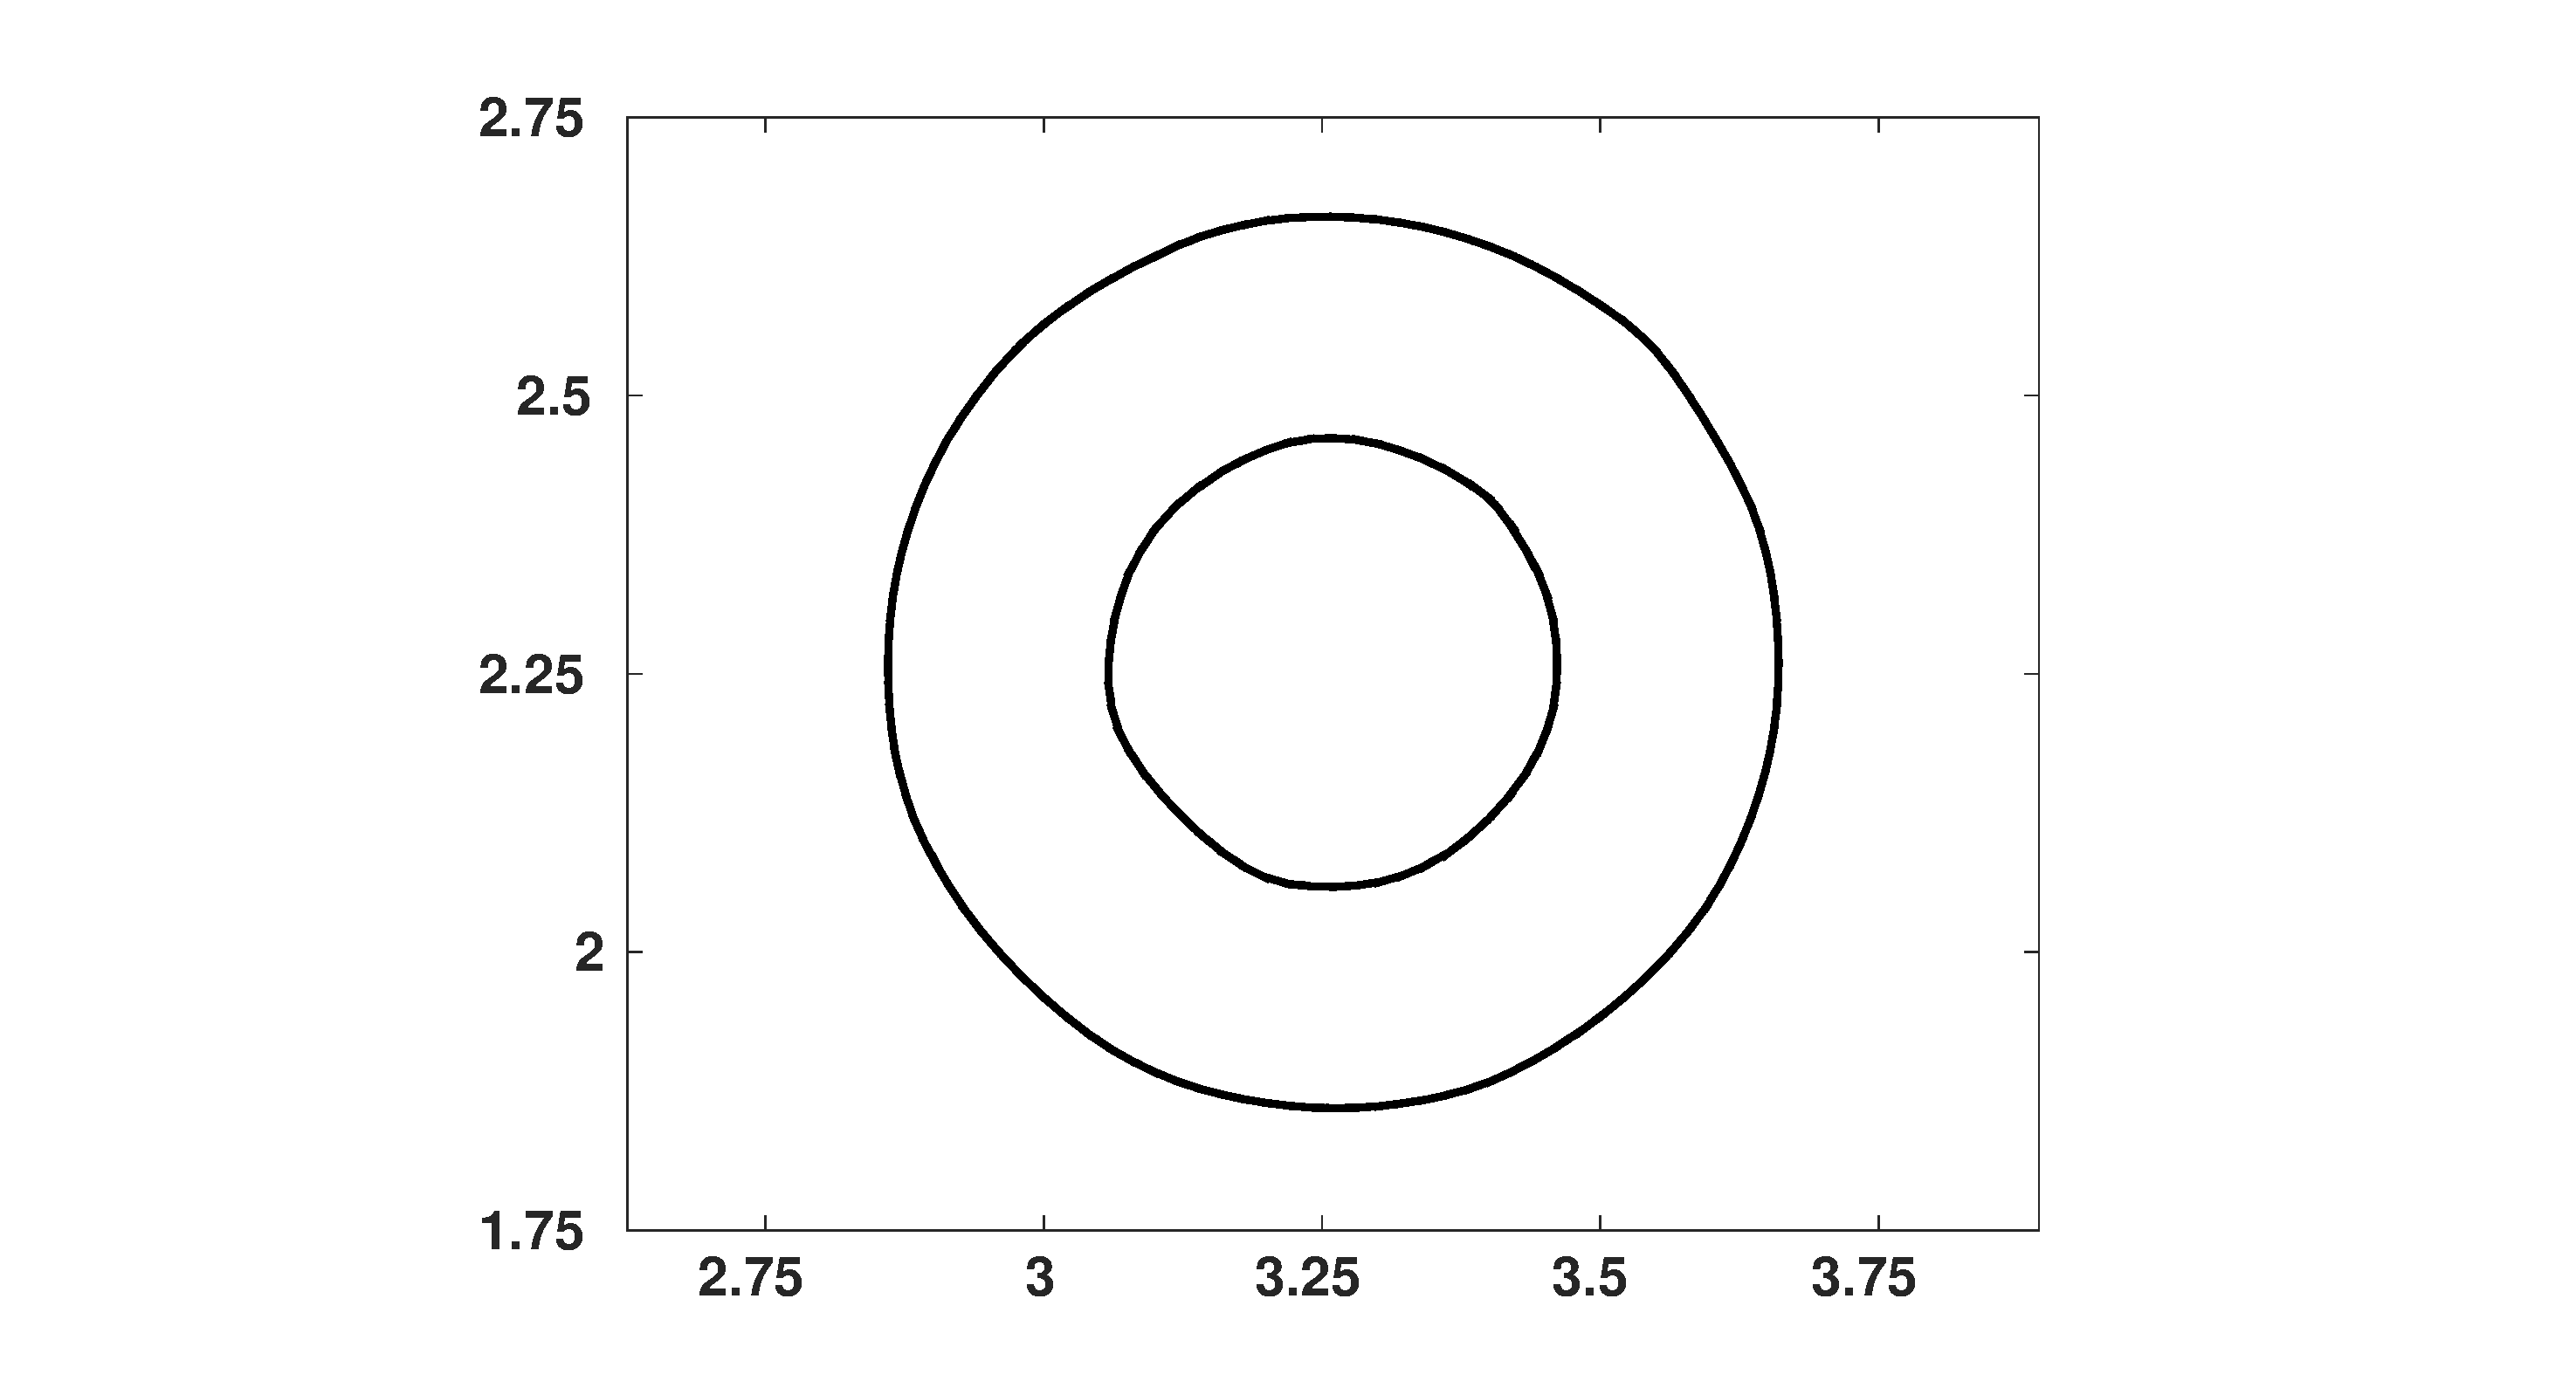
\includegraphics[width=0.5\textwidth]{final504.eps}
      }
 \caption{Advection test for velocity field u=2,v=1}
\end{figure}

\subsection{Advection test for solid body rotation}
For solid body rotation test a slotted circle configuration is taken from \cite{Zalesak1979}, the center of slotted circle is at
(2.0,2.75) and diameter is 1.0. The length and width of slot is 0.6 and 0.12 respectively.(Figure \ref{Fig:rotation} and \ref{Fig:rotation2})  
The refinement of the domain which is [0,4] x [0,4] is 200 x 200 . A velocity field is given by $u=-\Omega(y-y_0),v=\Omega(x-x_0)$, 
where axis of rotation passes through the $(x_0,y_0)$ and normal to the x-y plane. $\Omega$ is the angular velocity. 
Here $\Omega = 0.5$ and $(x_0,y_0)$ is $(2,2)$. The time step is 0.005.
\begin{enumerate}
 \item Domain: [0,4] x [0,4]
 \item Grid Size: 200 x 200
 \item Radius of circle :0.5
 \item Center : (2.0,2.75)
 \item Velocity field:  $u=-0.5(y-2),v=0.5(x-2)$
\end{enumerate}

% 
\begin{figure}
  \subfloat[After advecting 628 steps ]{%
      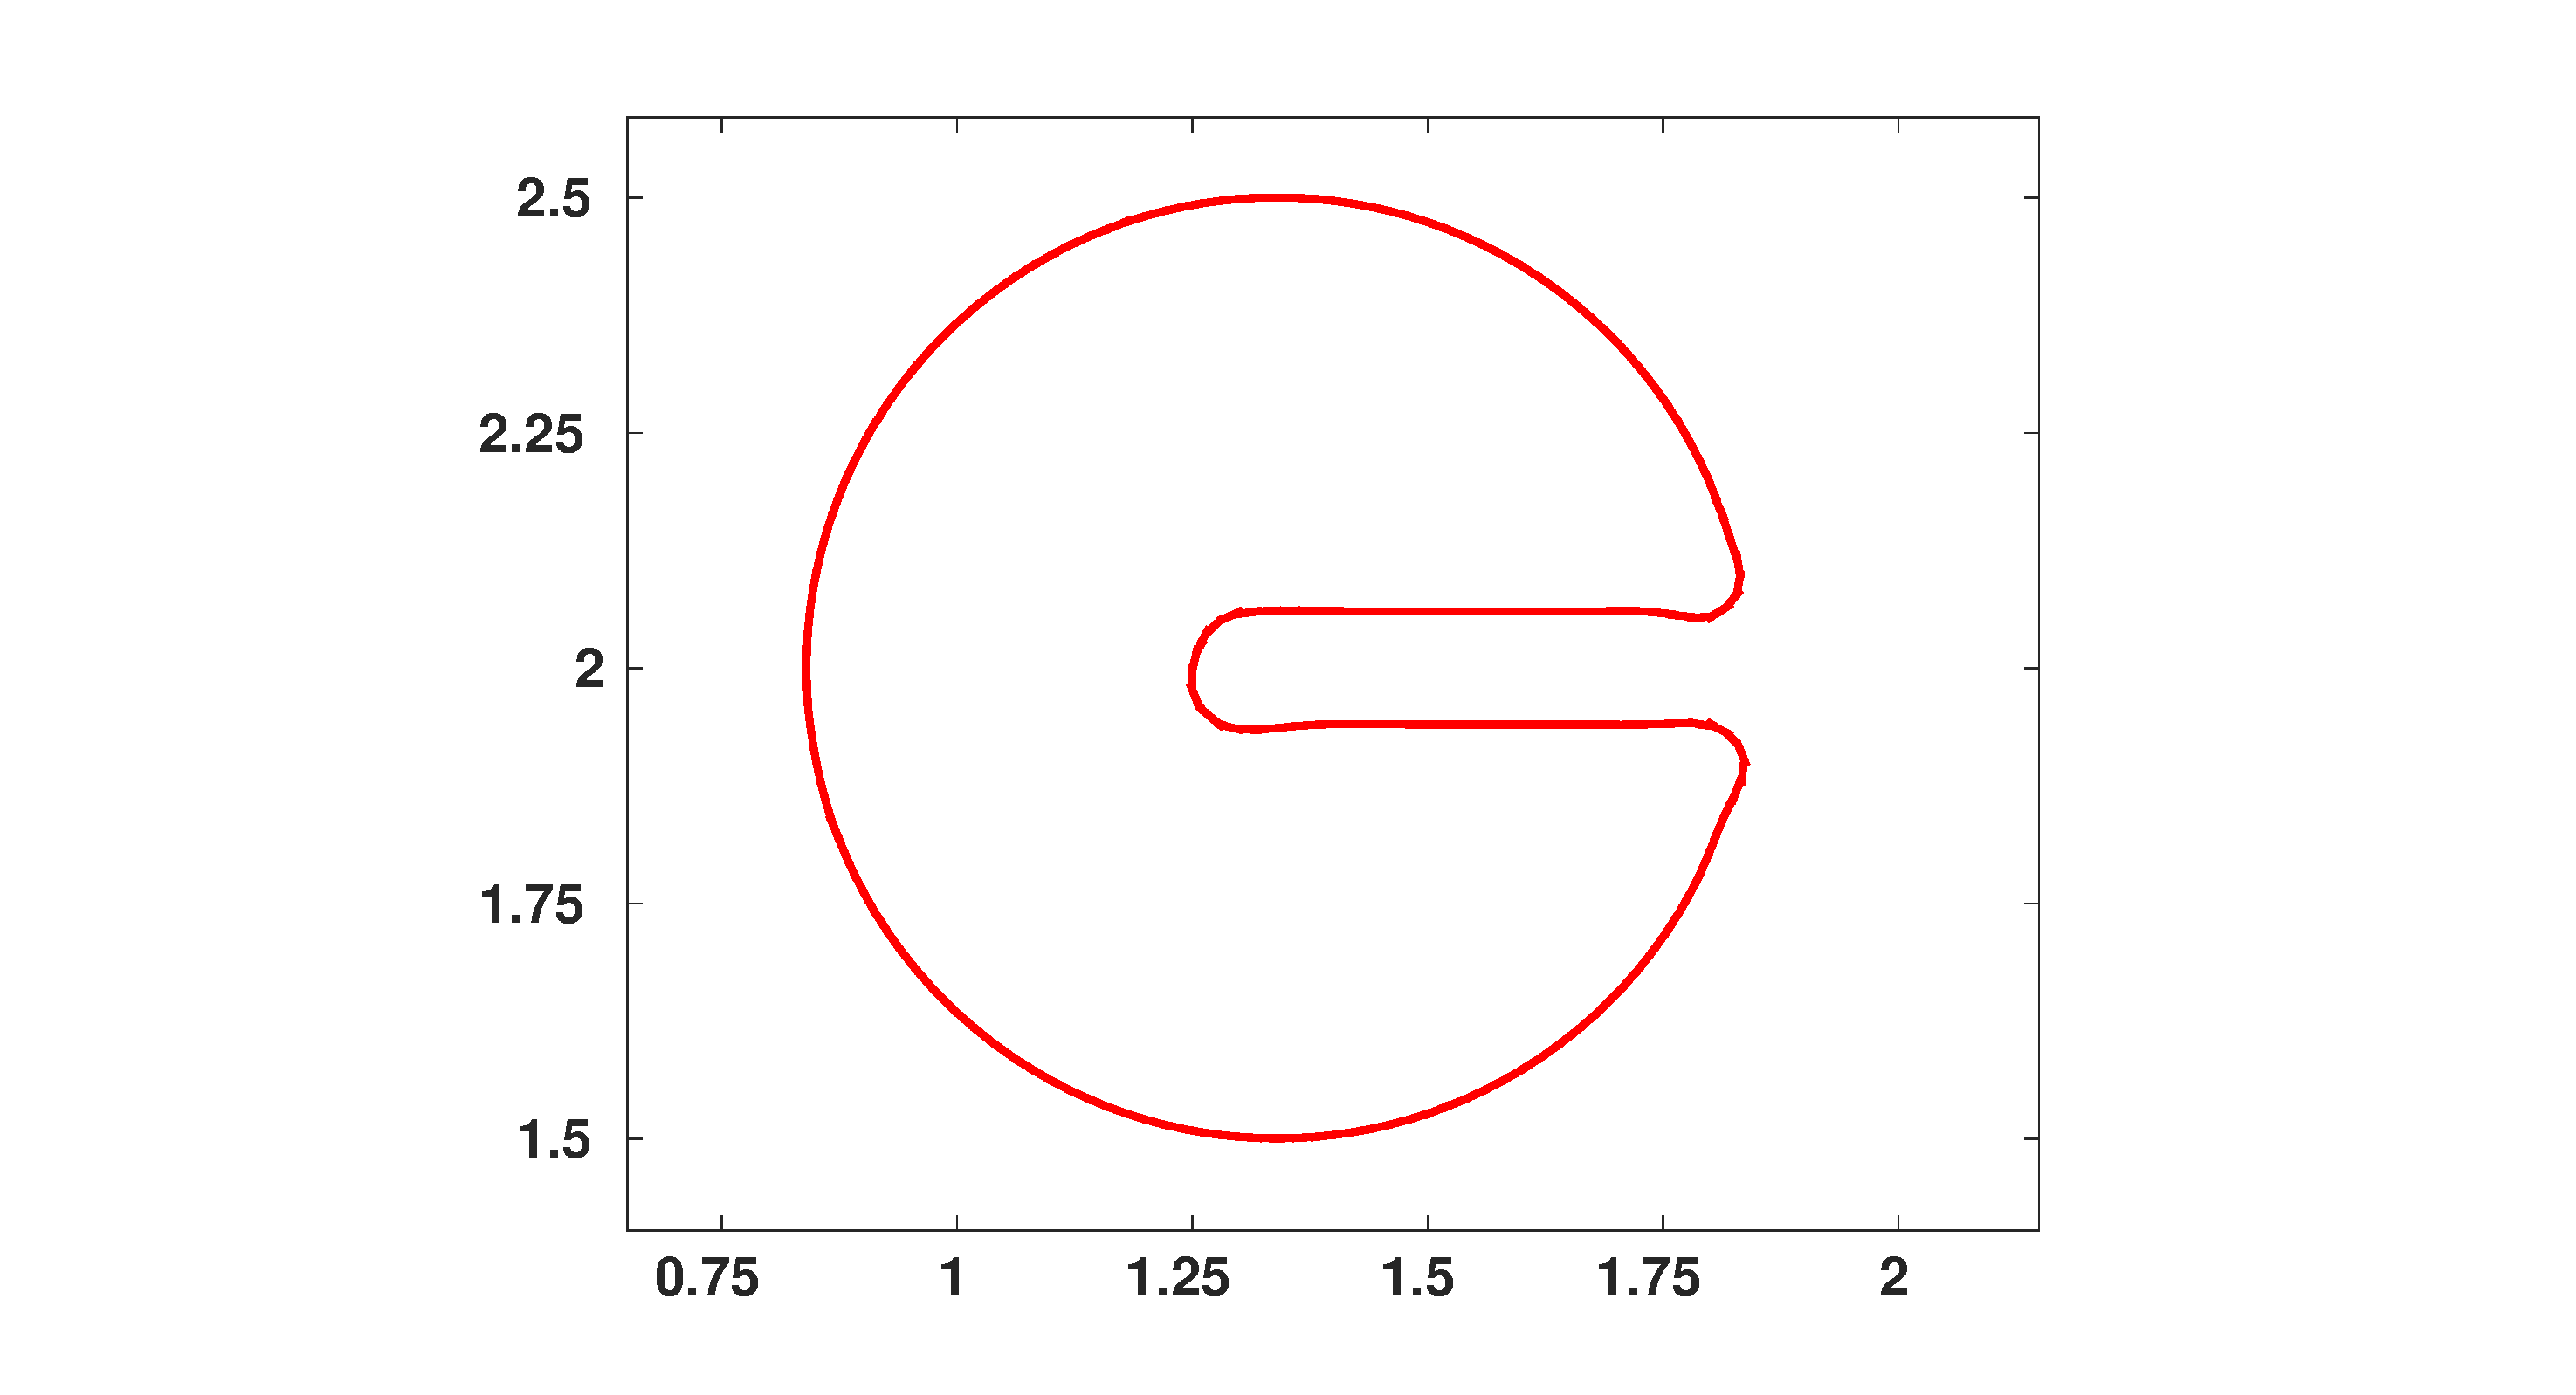
\includegraphics[width=0.5\textwidth]{SC_628.eps}
      }
     \subfloat[After advecting 1256 steps ]{%
      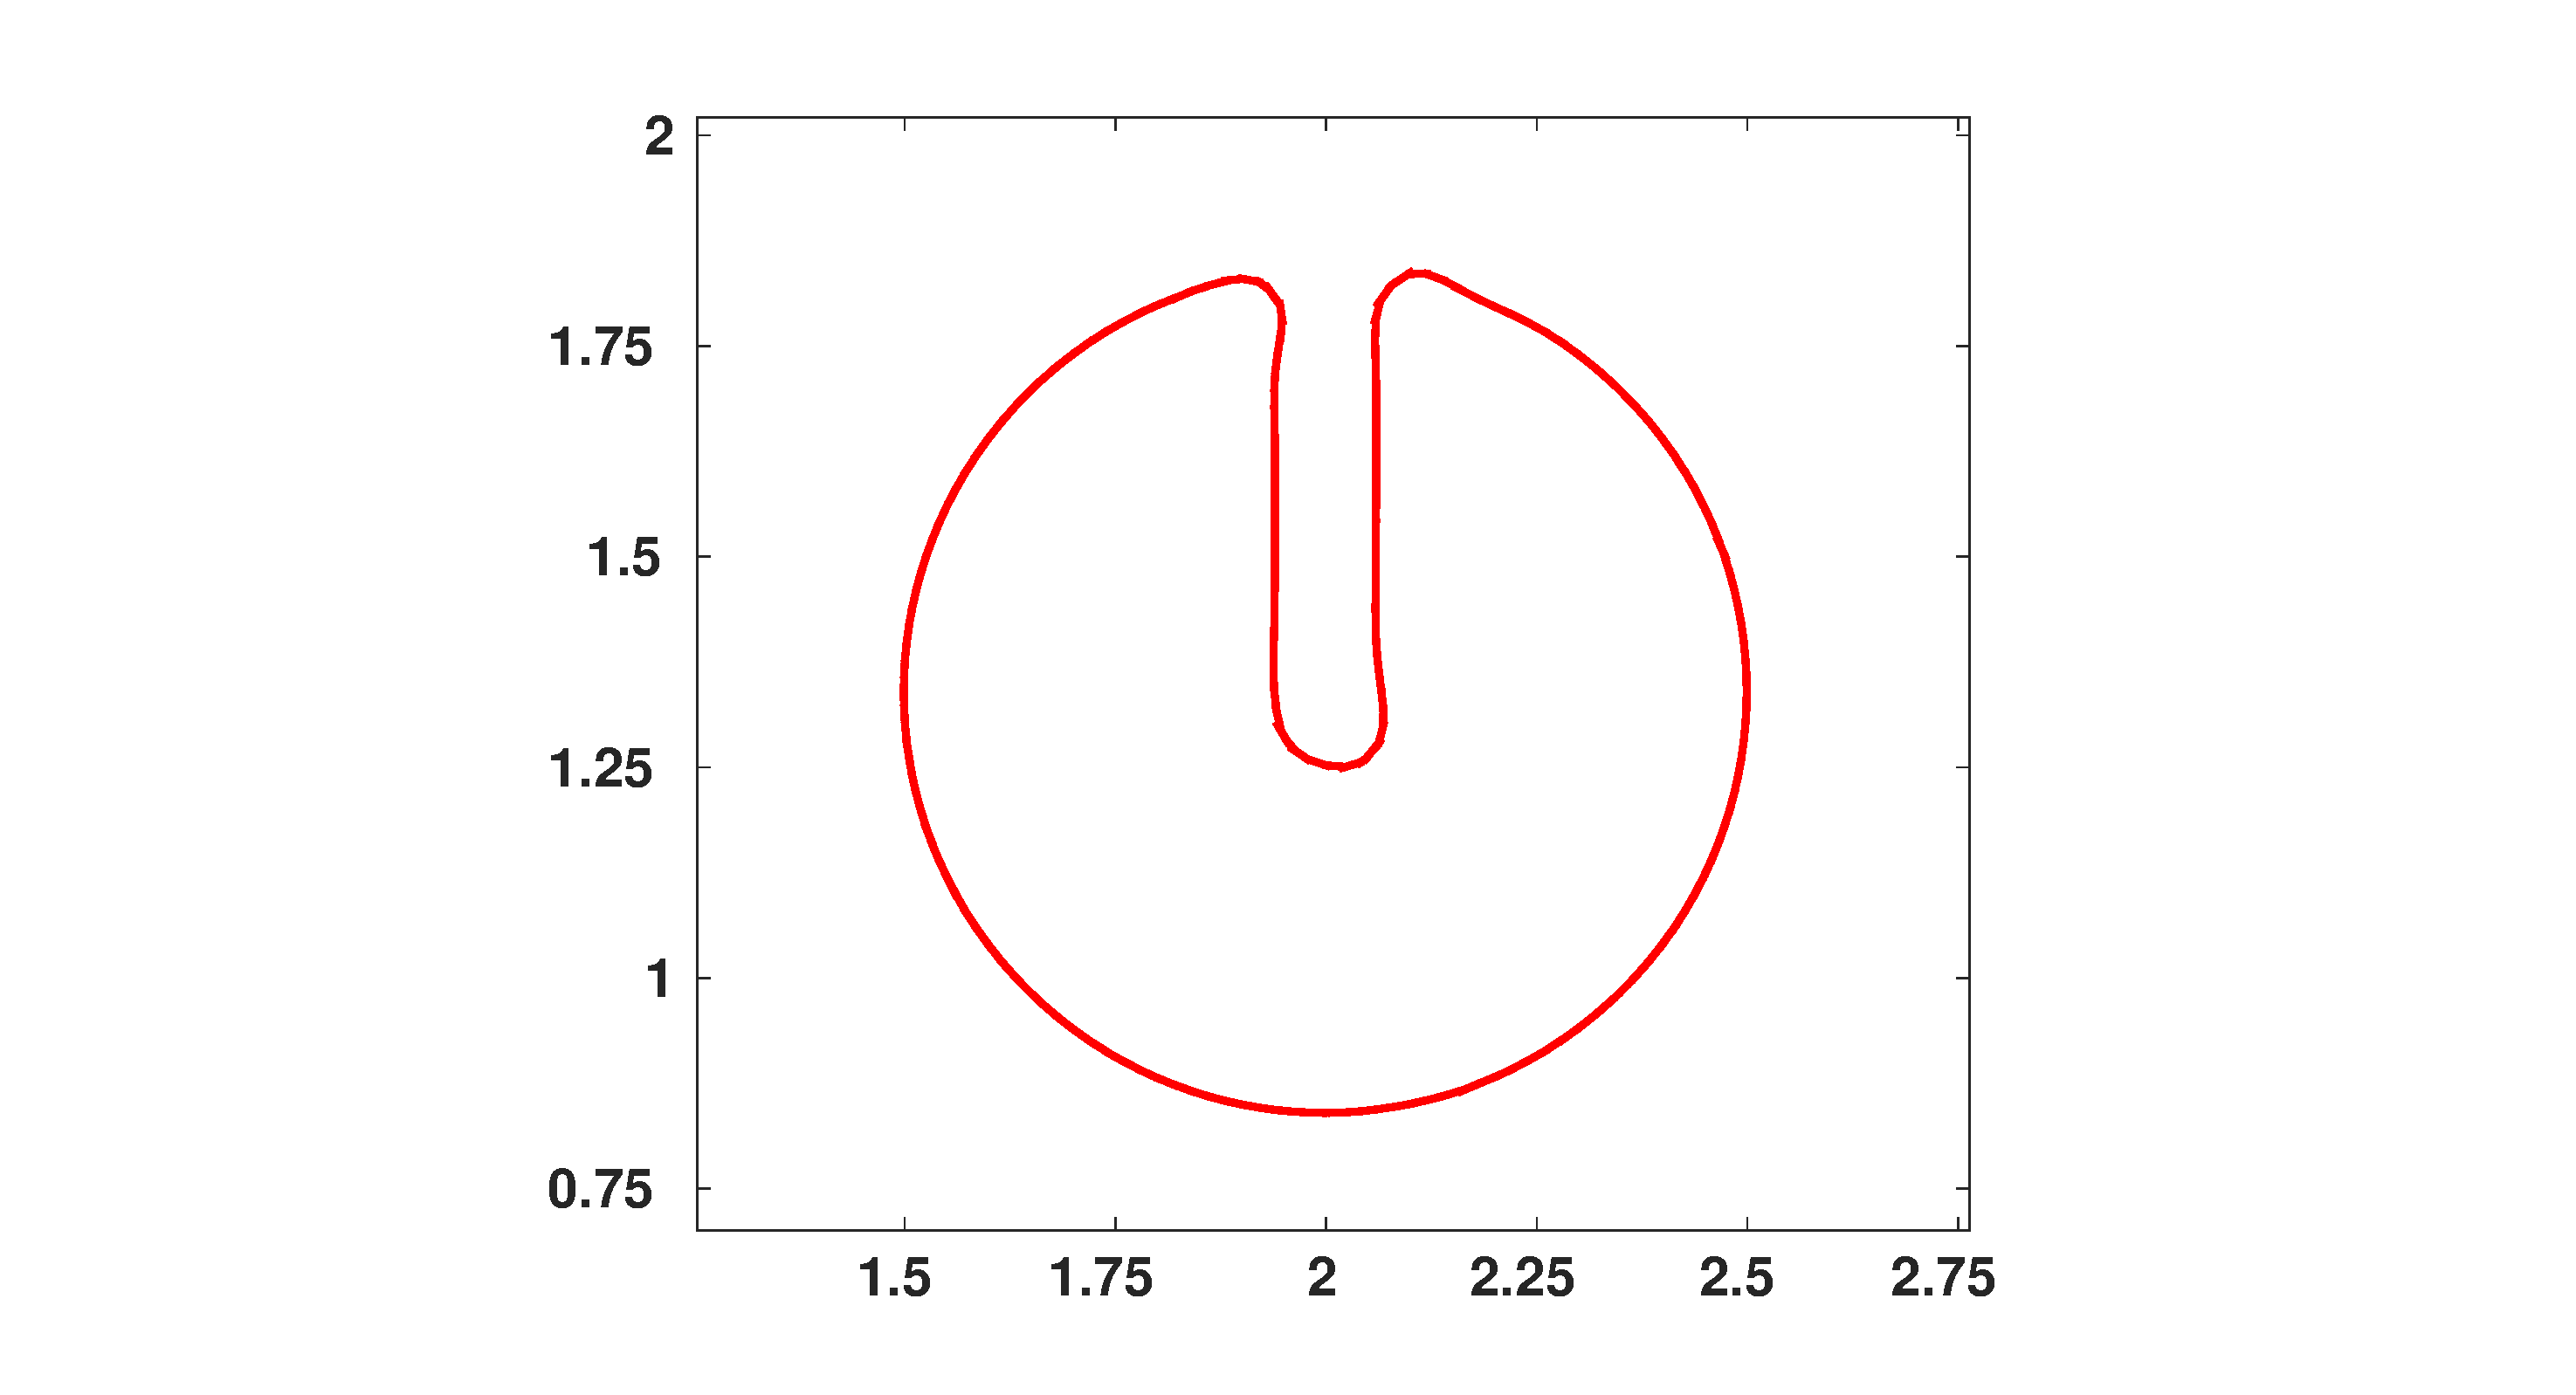
\includegraphics[width=0.5\textwidth]{SC_1256.eps}
      }\\
        \subfloat[After advecting 1885 steps ]{%
      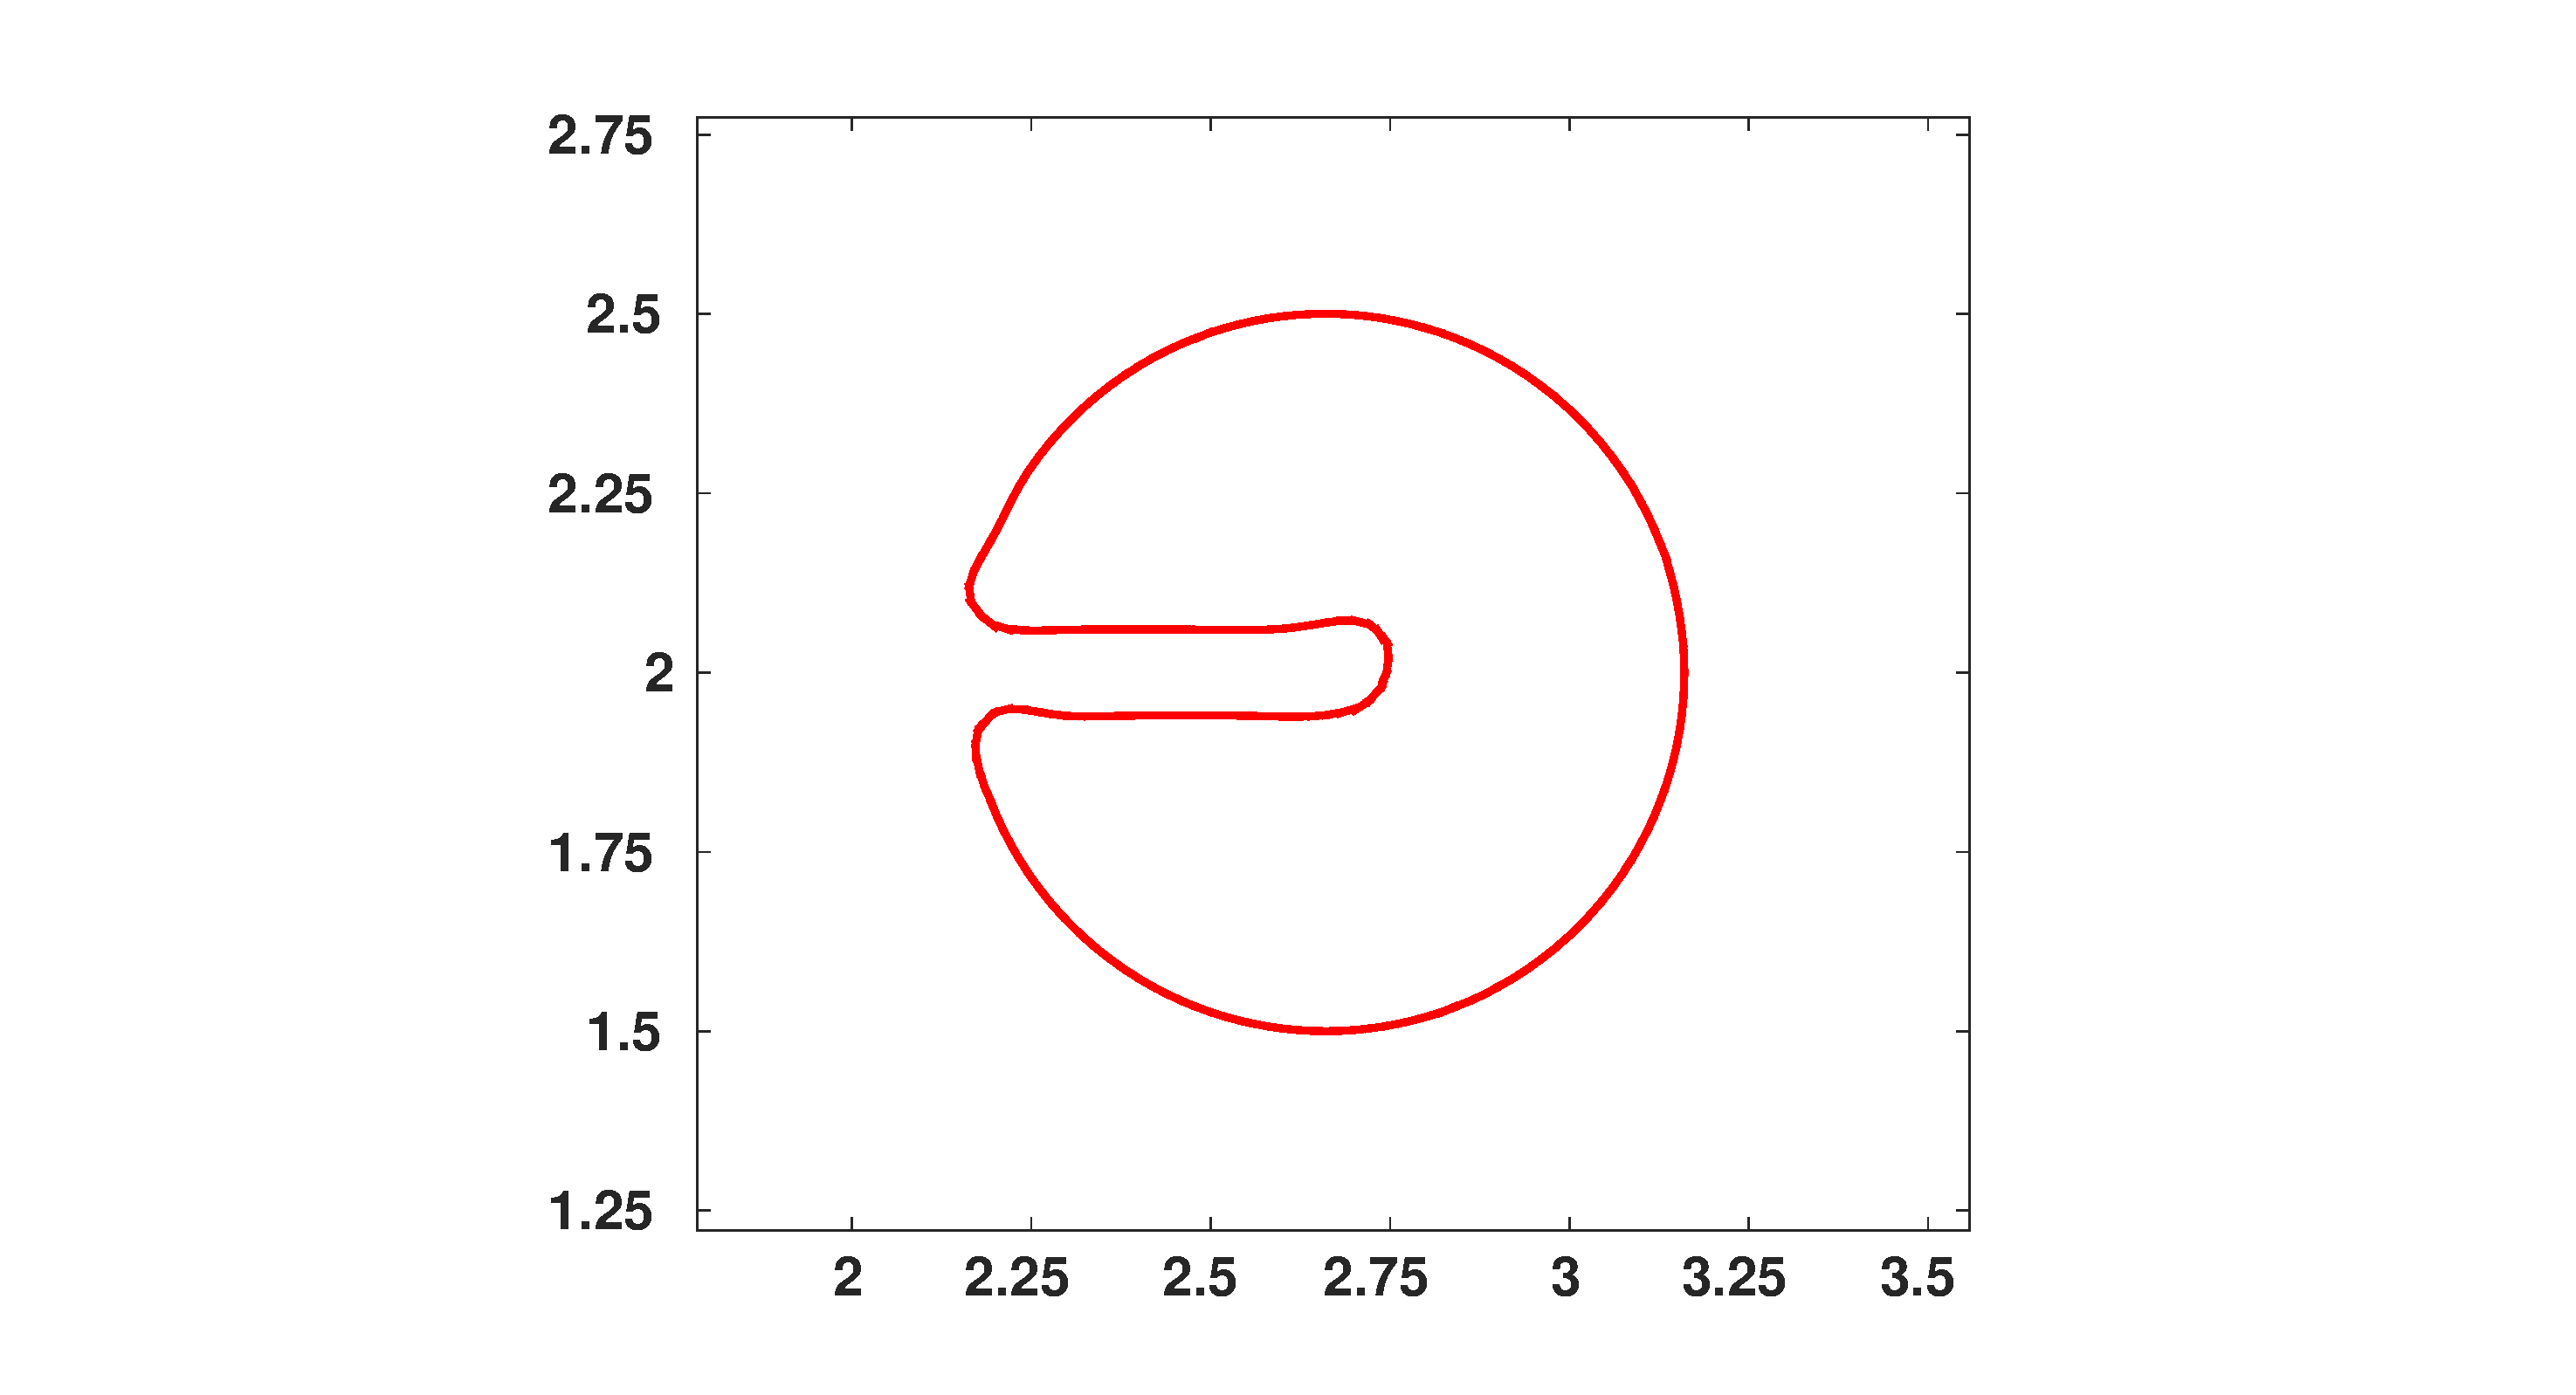
\includegraphics[width=0.5\textwidth]{SC_1885.eps}
      }
        \subfloat[After advecting 2513 steps ]{%
      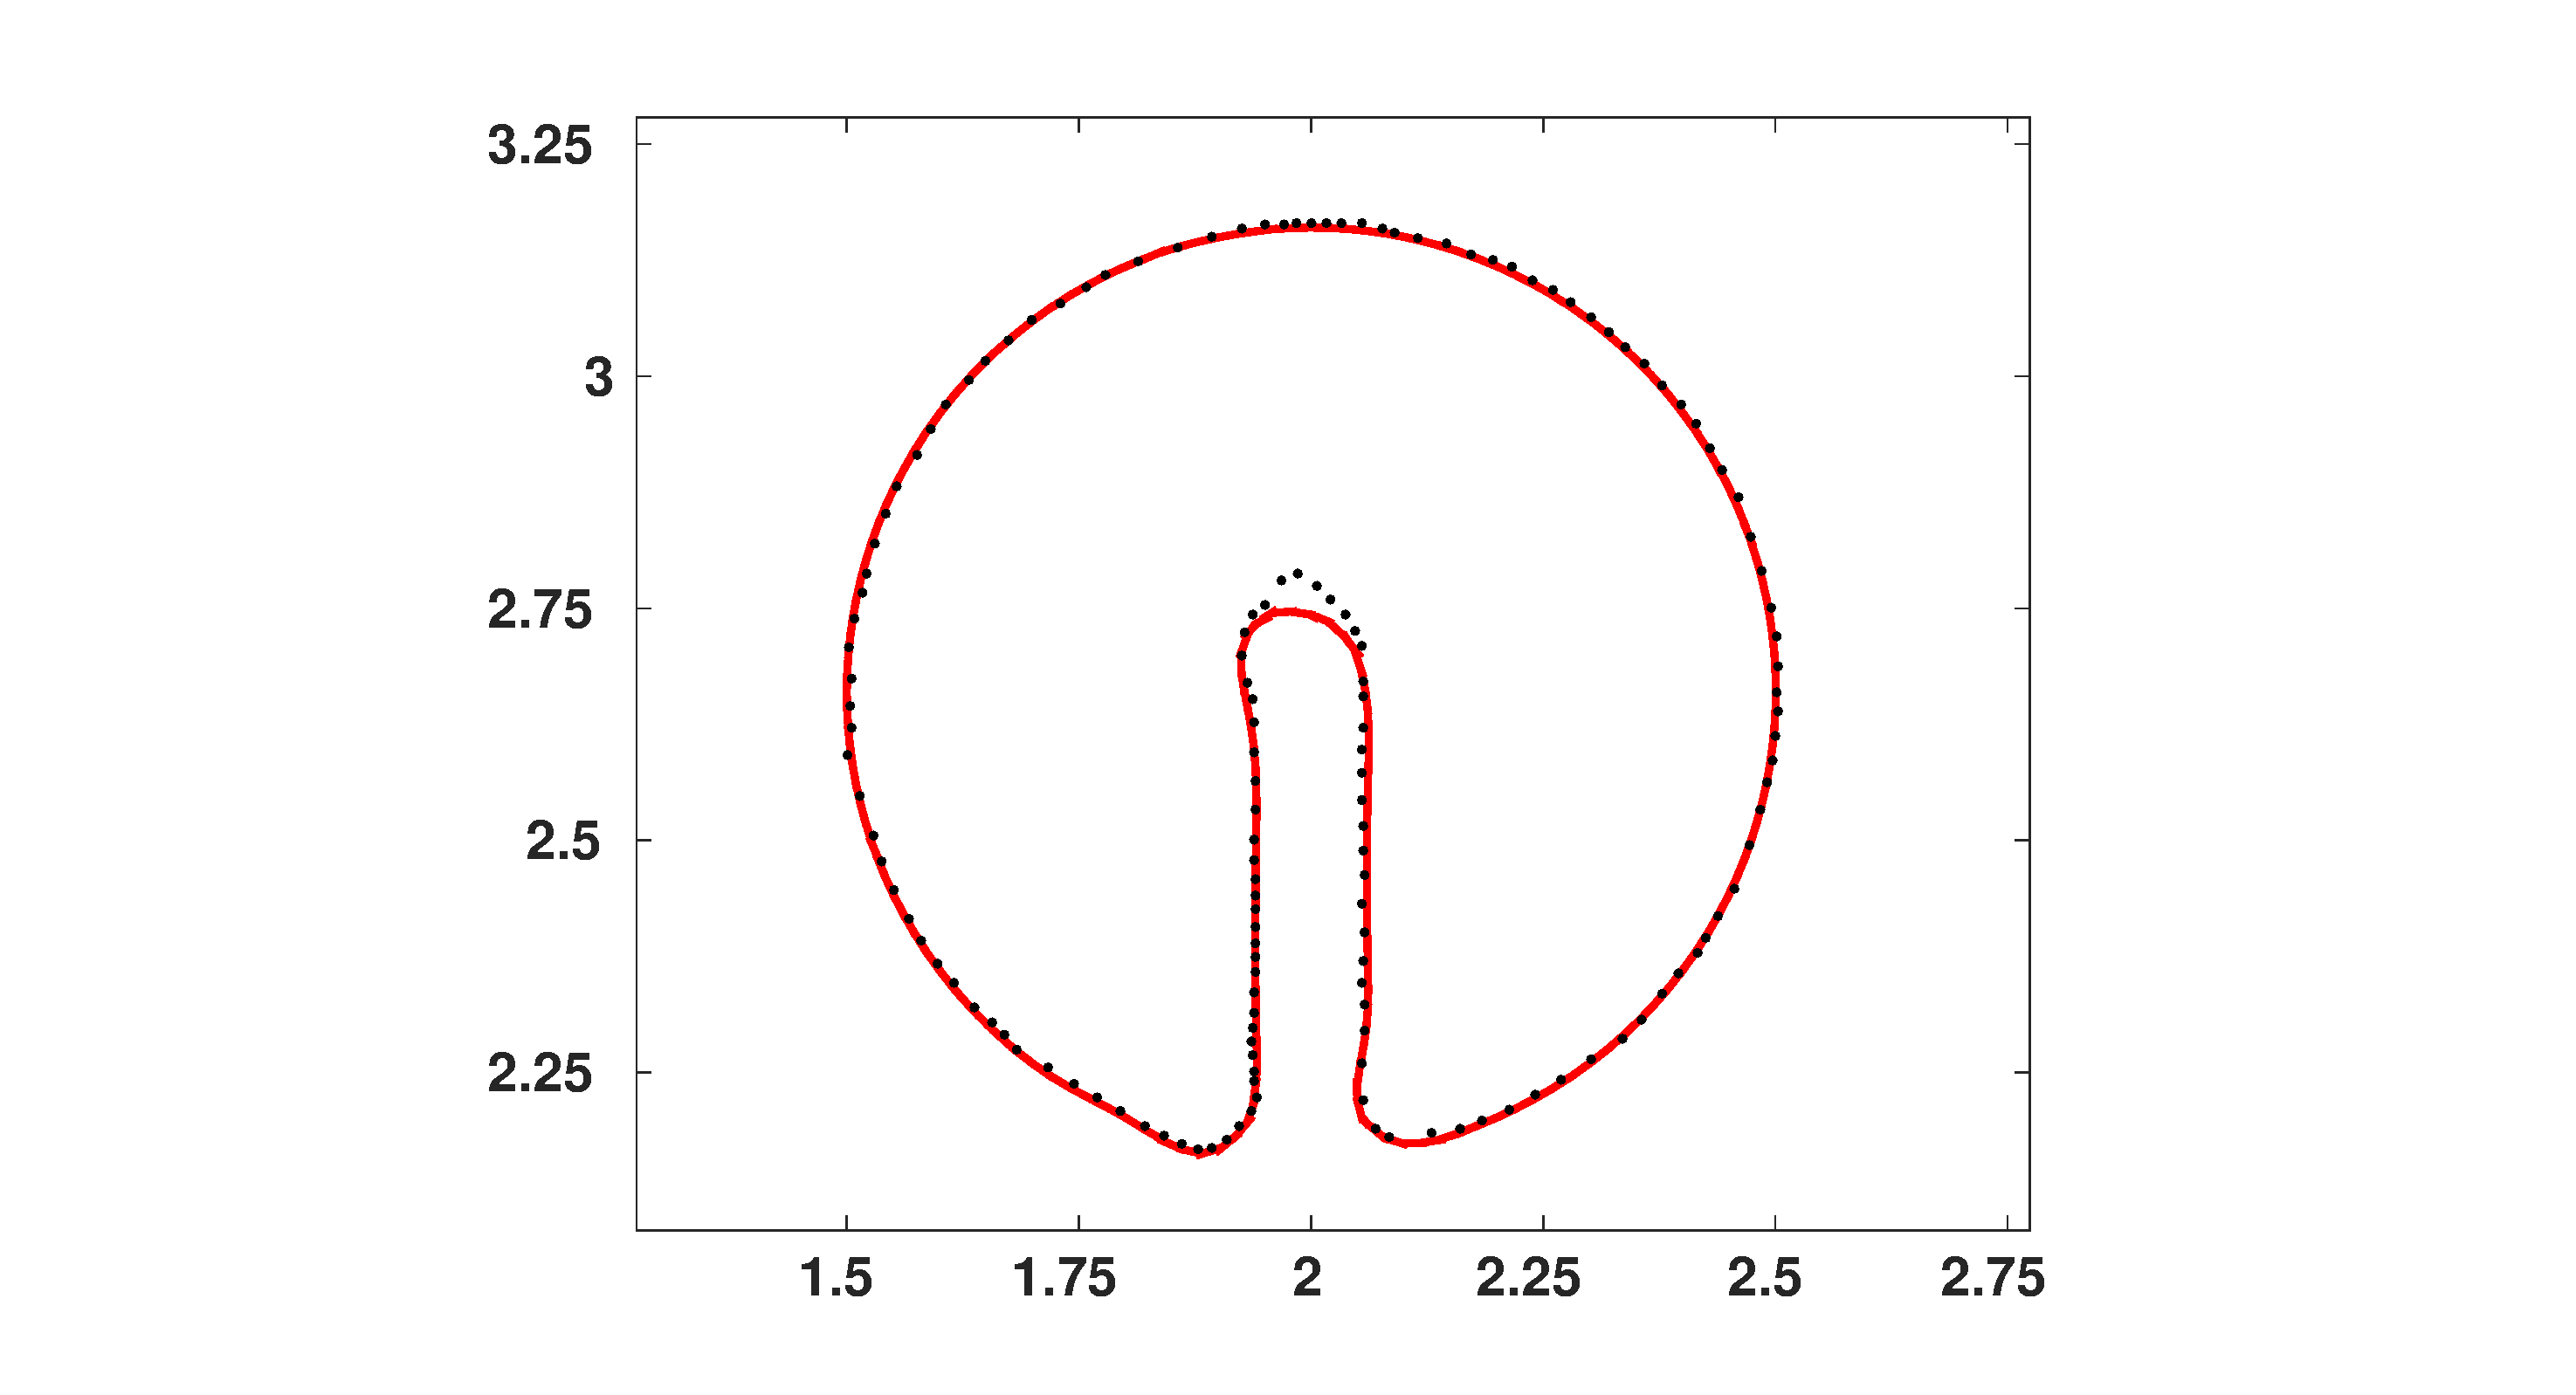
\includegraphics[width=0.5\textwidth]{SC_2513.eps}
      }
 \caption{Advection test result for solid body rotation}
 \label{Fig:rotation2}
\end{figure}
% 
\begin{figure}
 \centering 
 \subfloat[Initial Condition for solid body rotation test ]{%
      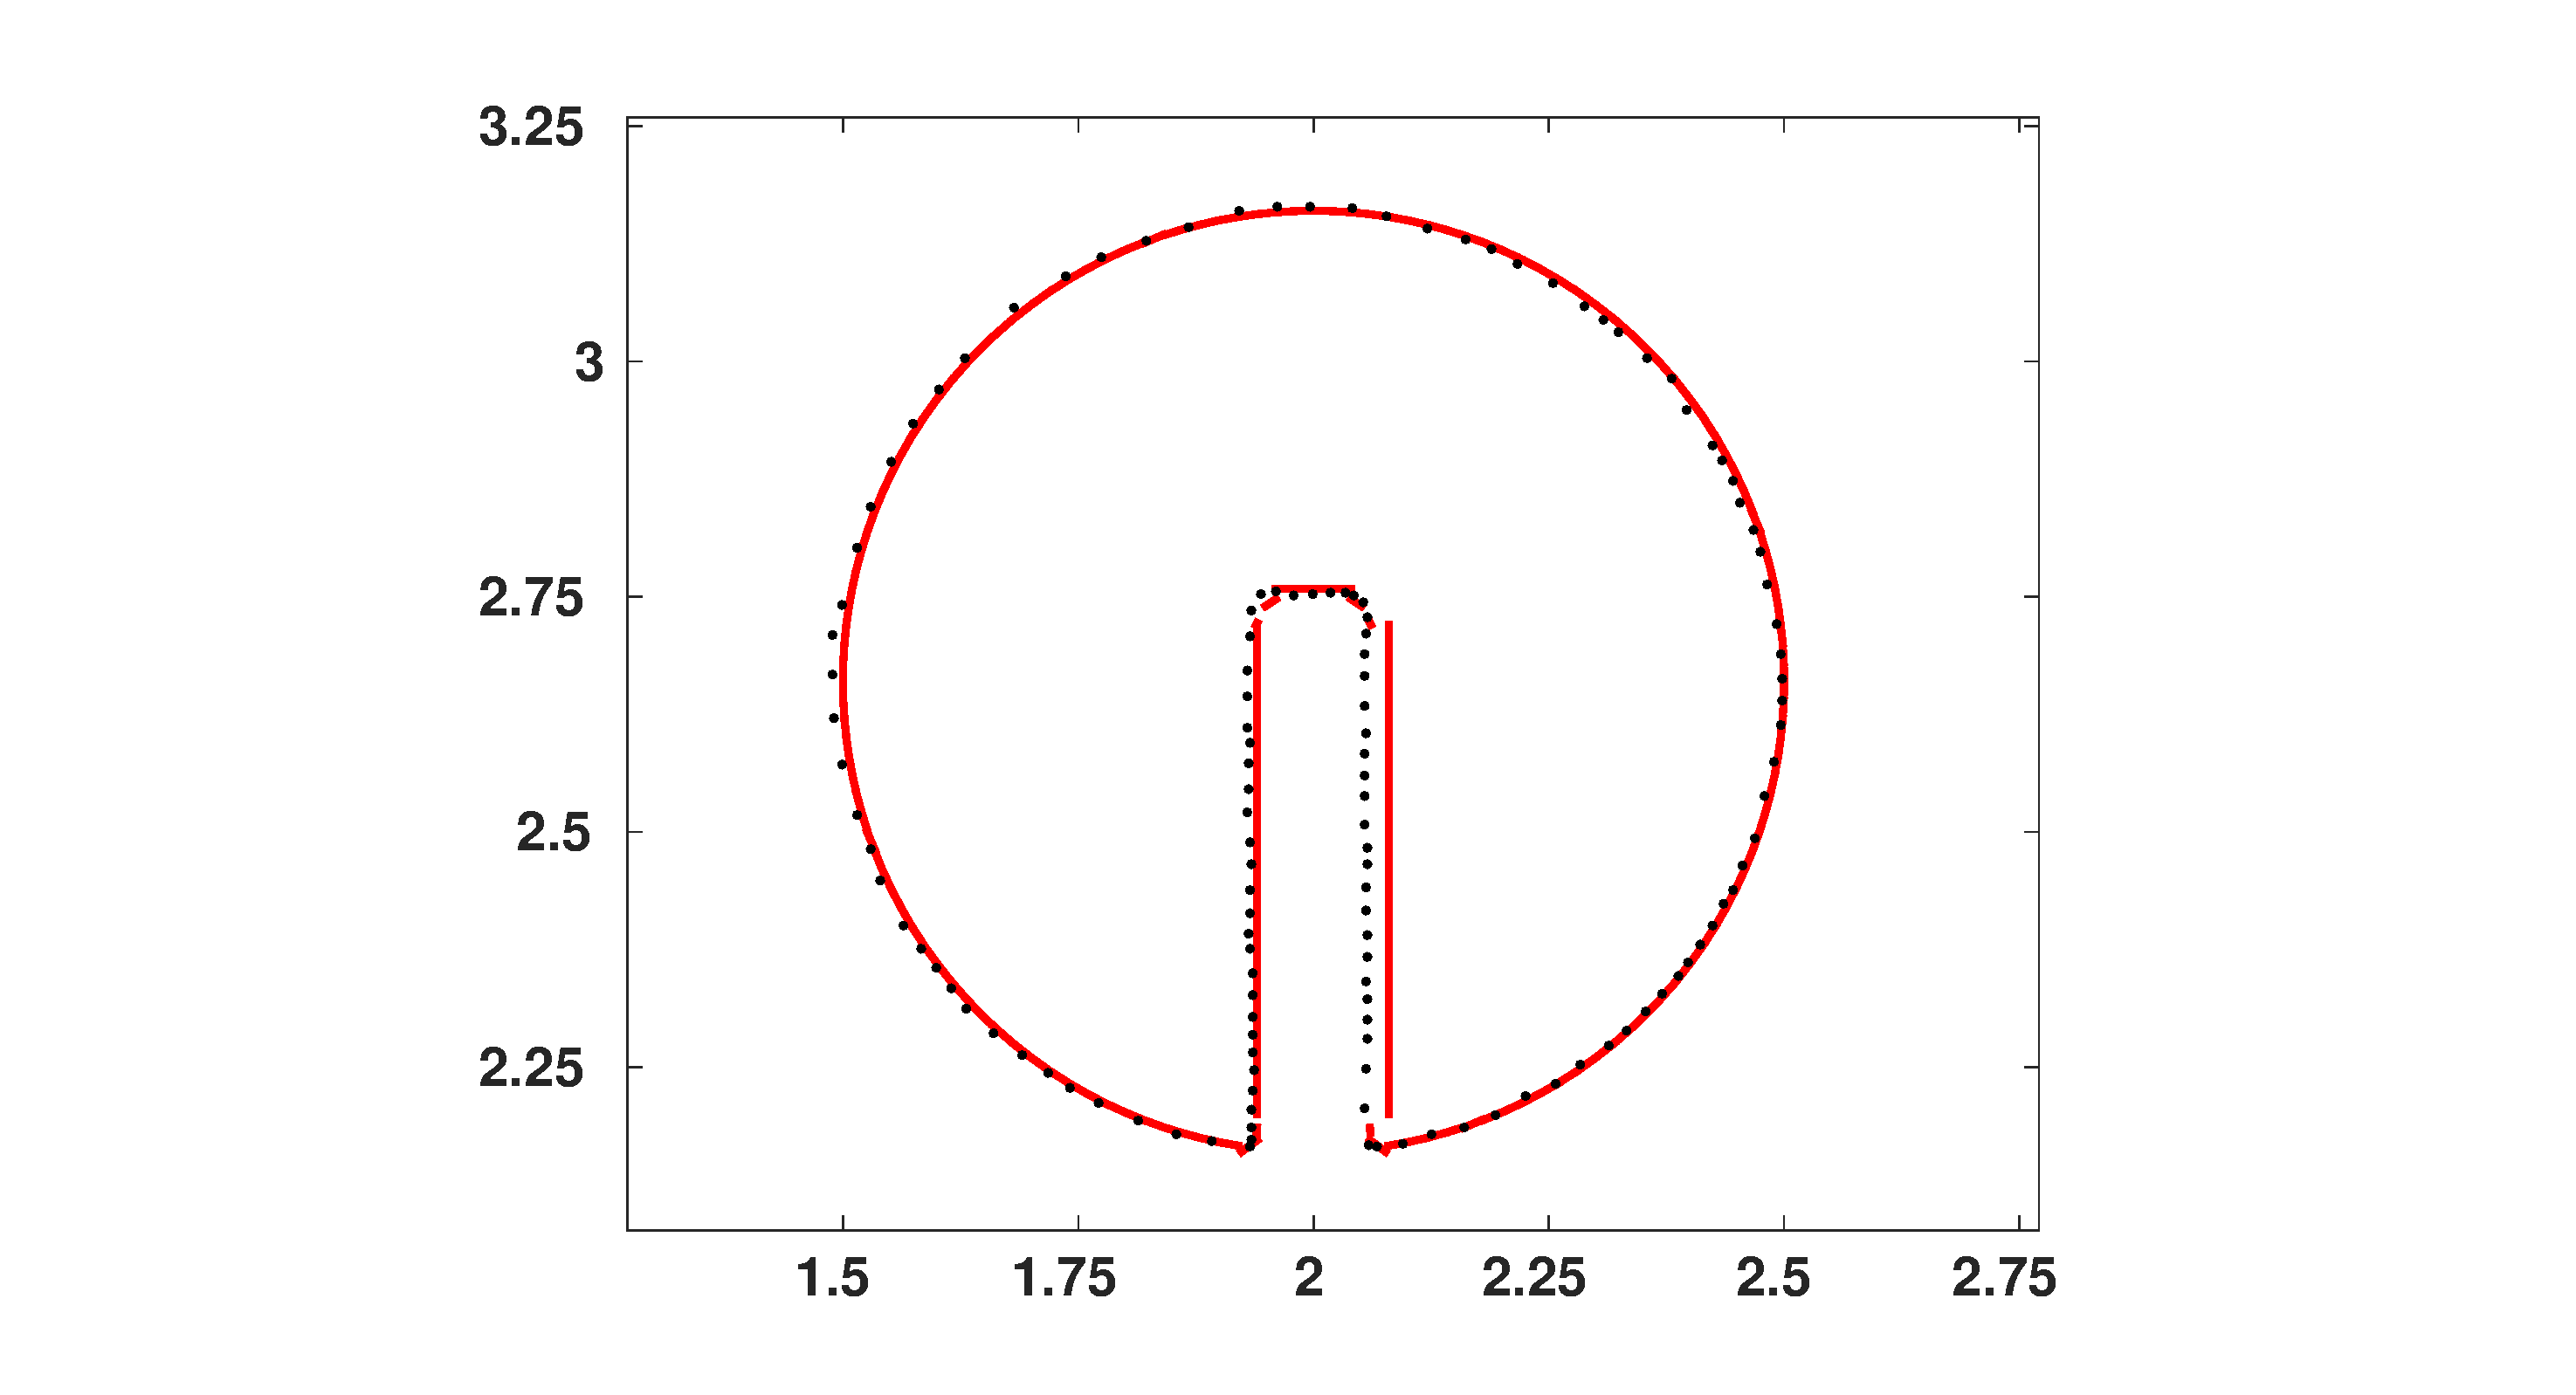
\includegraphics[width=0.5\textwidth]{SC_IC.eps}
      } 
  \subfloat[After one full rotation ]{%
      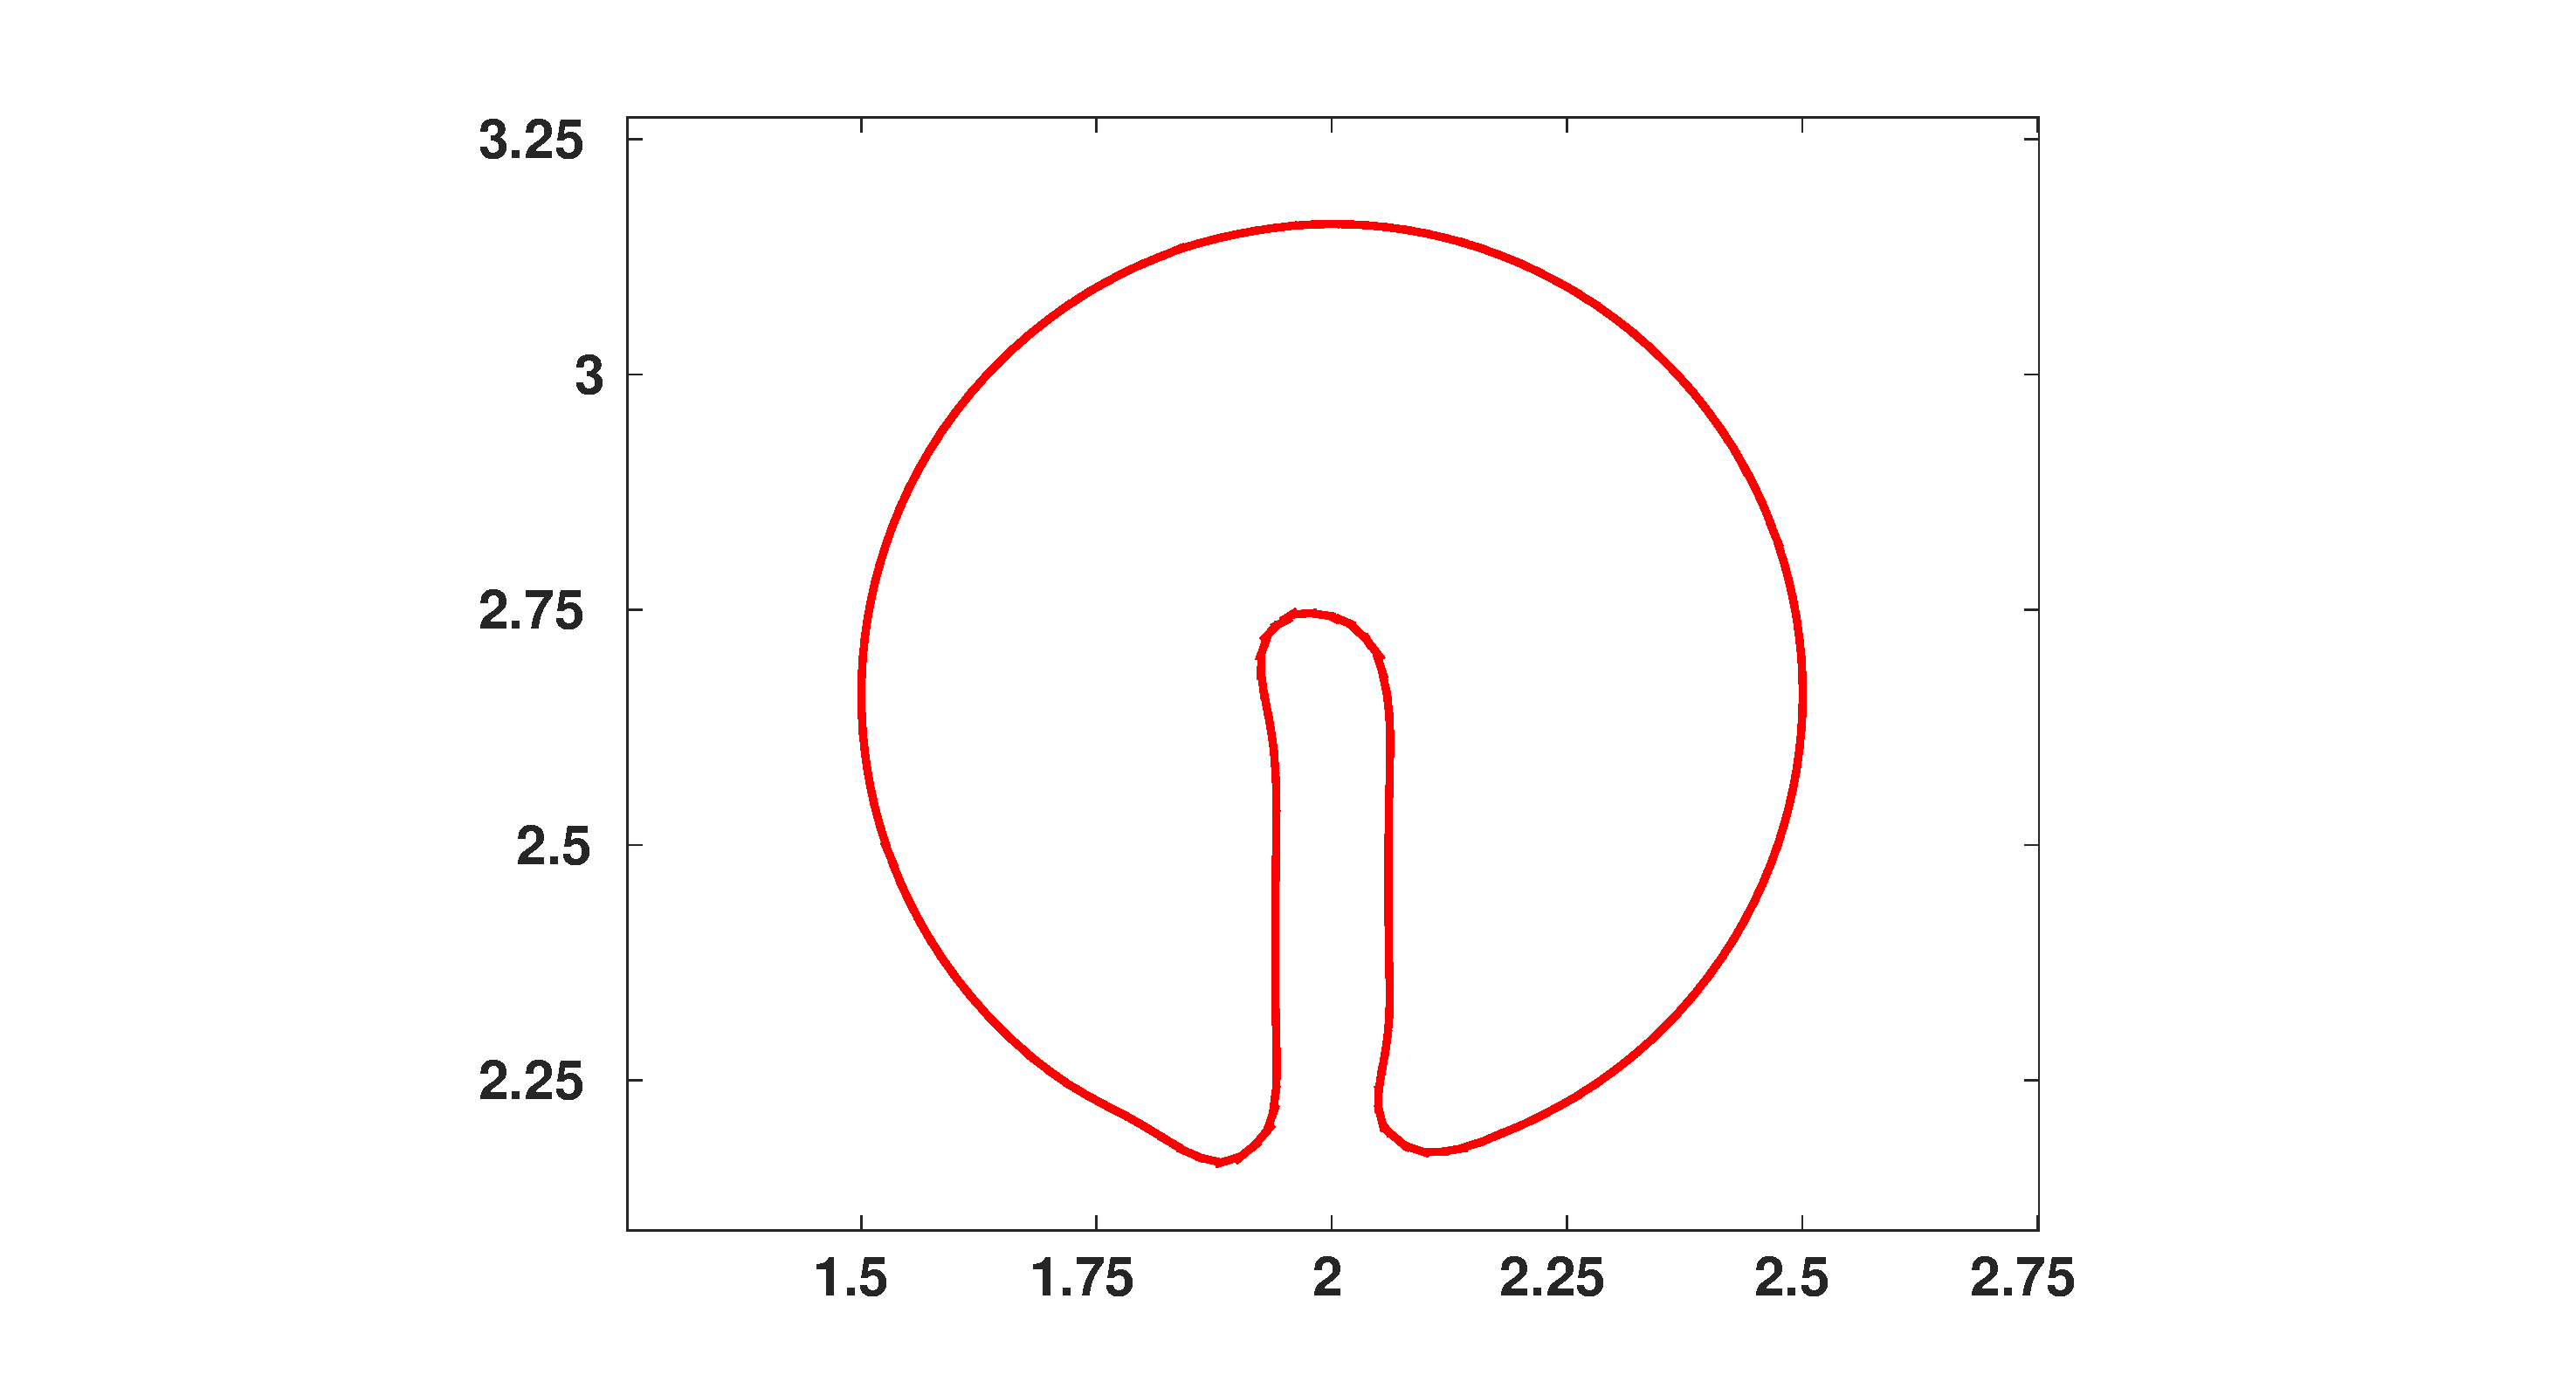
\includegraphics[width=0.5\textwidth]{SC_2513O.eps}
      }
 \caption{Comparison with \cite{Rudman1997} results. (Red LVIRA and Blue \cite{Rudman1997} data)}
 \label{Fig:rotation}
\end{figure}

\subsection{Shear Test}
The real problems typically encounters the interface deformation, which includes merging and deformation. Hence the algorithm has to be 
tested for shear velocity field (Figure \ref{Fig:shear}). The shear test problem verified with \cite{Gerlach2006}. (Figure \ref{Fig:shear_comparison}) 

   \begin{enumerate}
 \item Domain: [0,$\pi$] x [0,$\pi$]
 \item Grid Size: 100 x 100
 \item Radius of circle :$\frac{\pi}{5}$
 \item Center : $(\pi/2,\pi/4)$
 \item Velocity field(Forward):  $u=sin x cos y, v=-cos x sin y$
  \item Velocity field(Backward):  $u=-sin x cos y,v=cos x sin y$
 \end{enumerate}
 
\begin{figure}
\centering
   \subfloat[Initial condition for shear test ]{%
      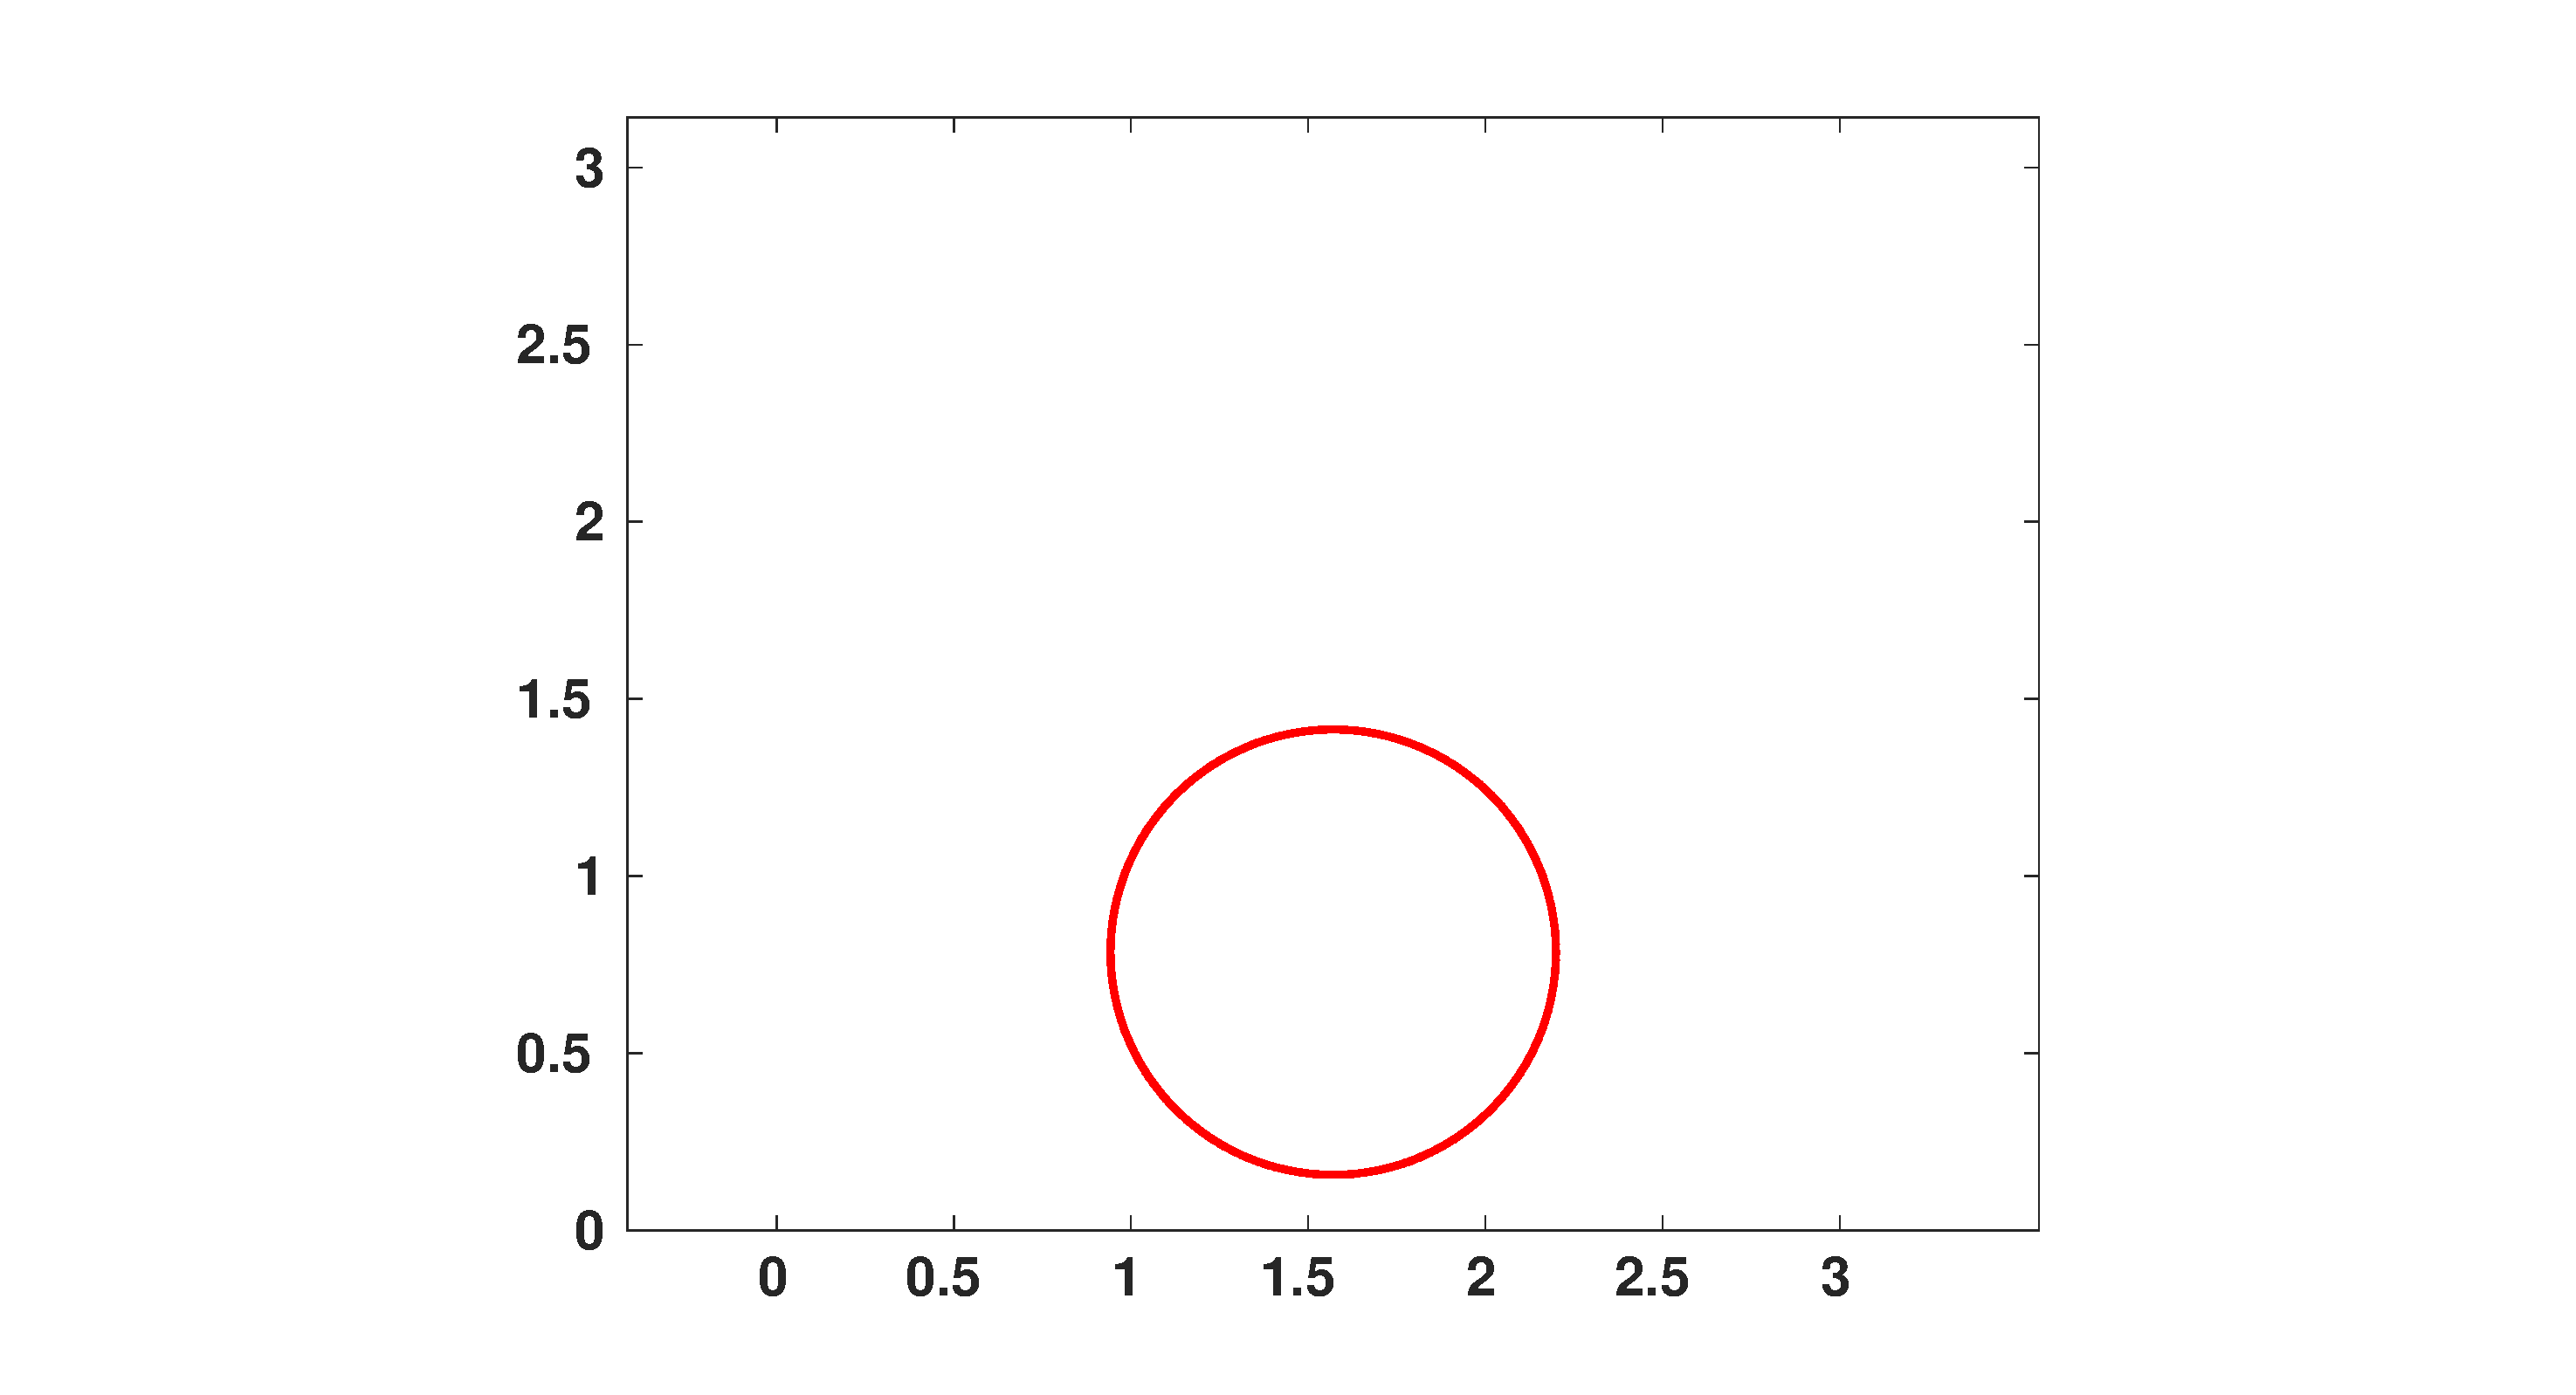
\includegraphics[width=0.5\textwidth]{shear_IC.eps}
      }
\subfloat[After advecting 250 steps ]{%
      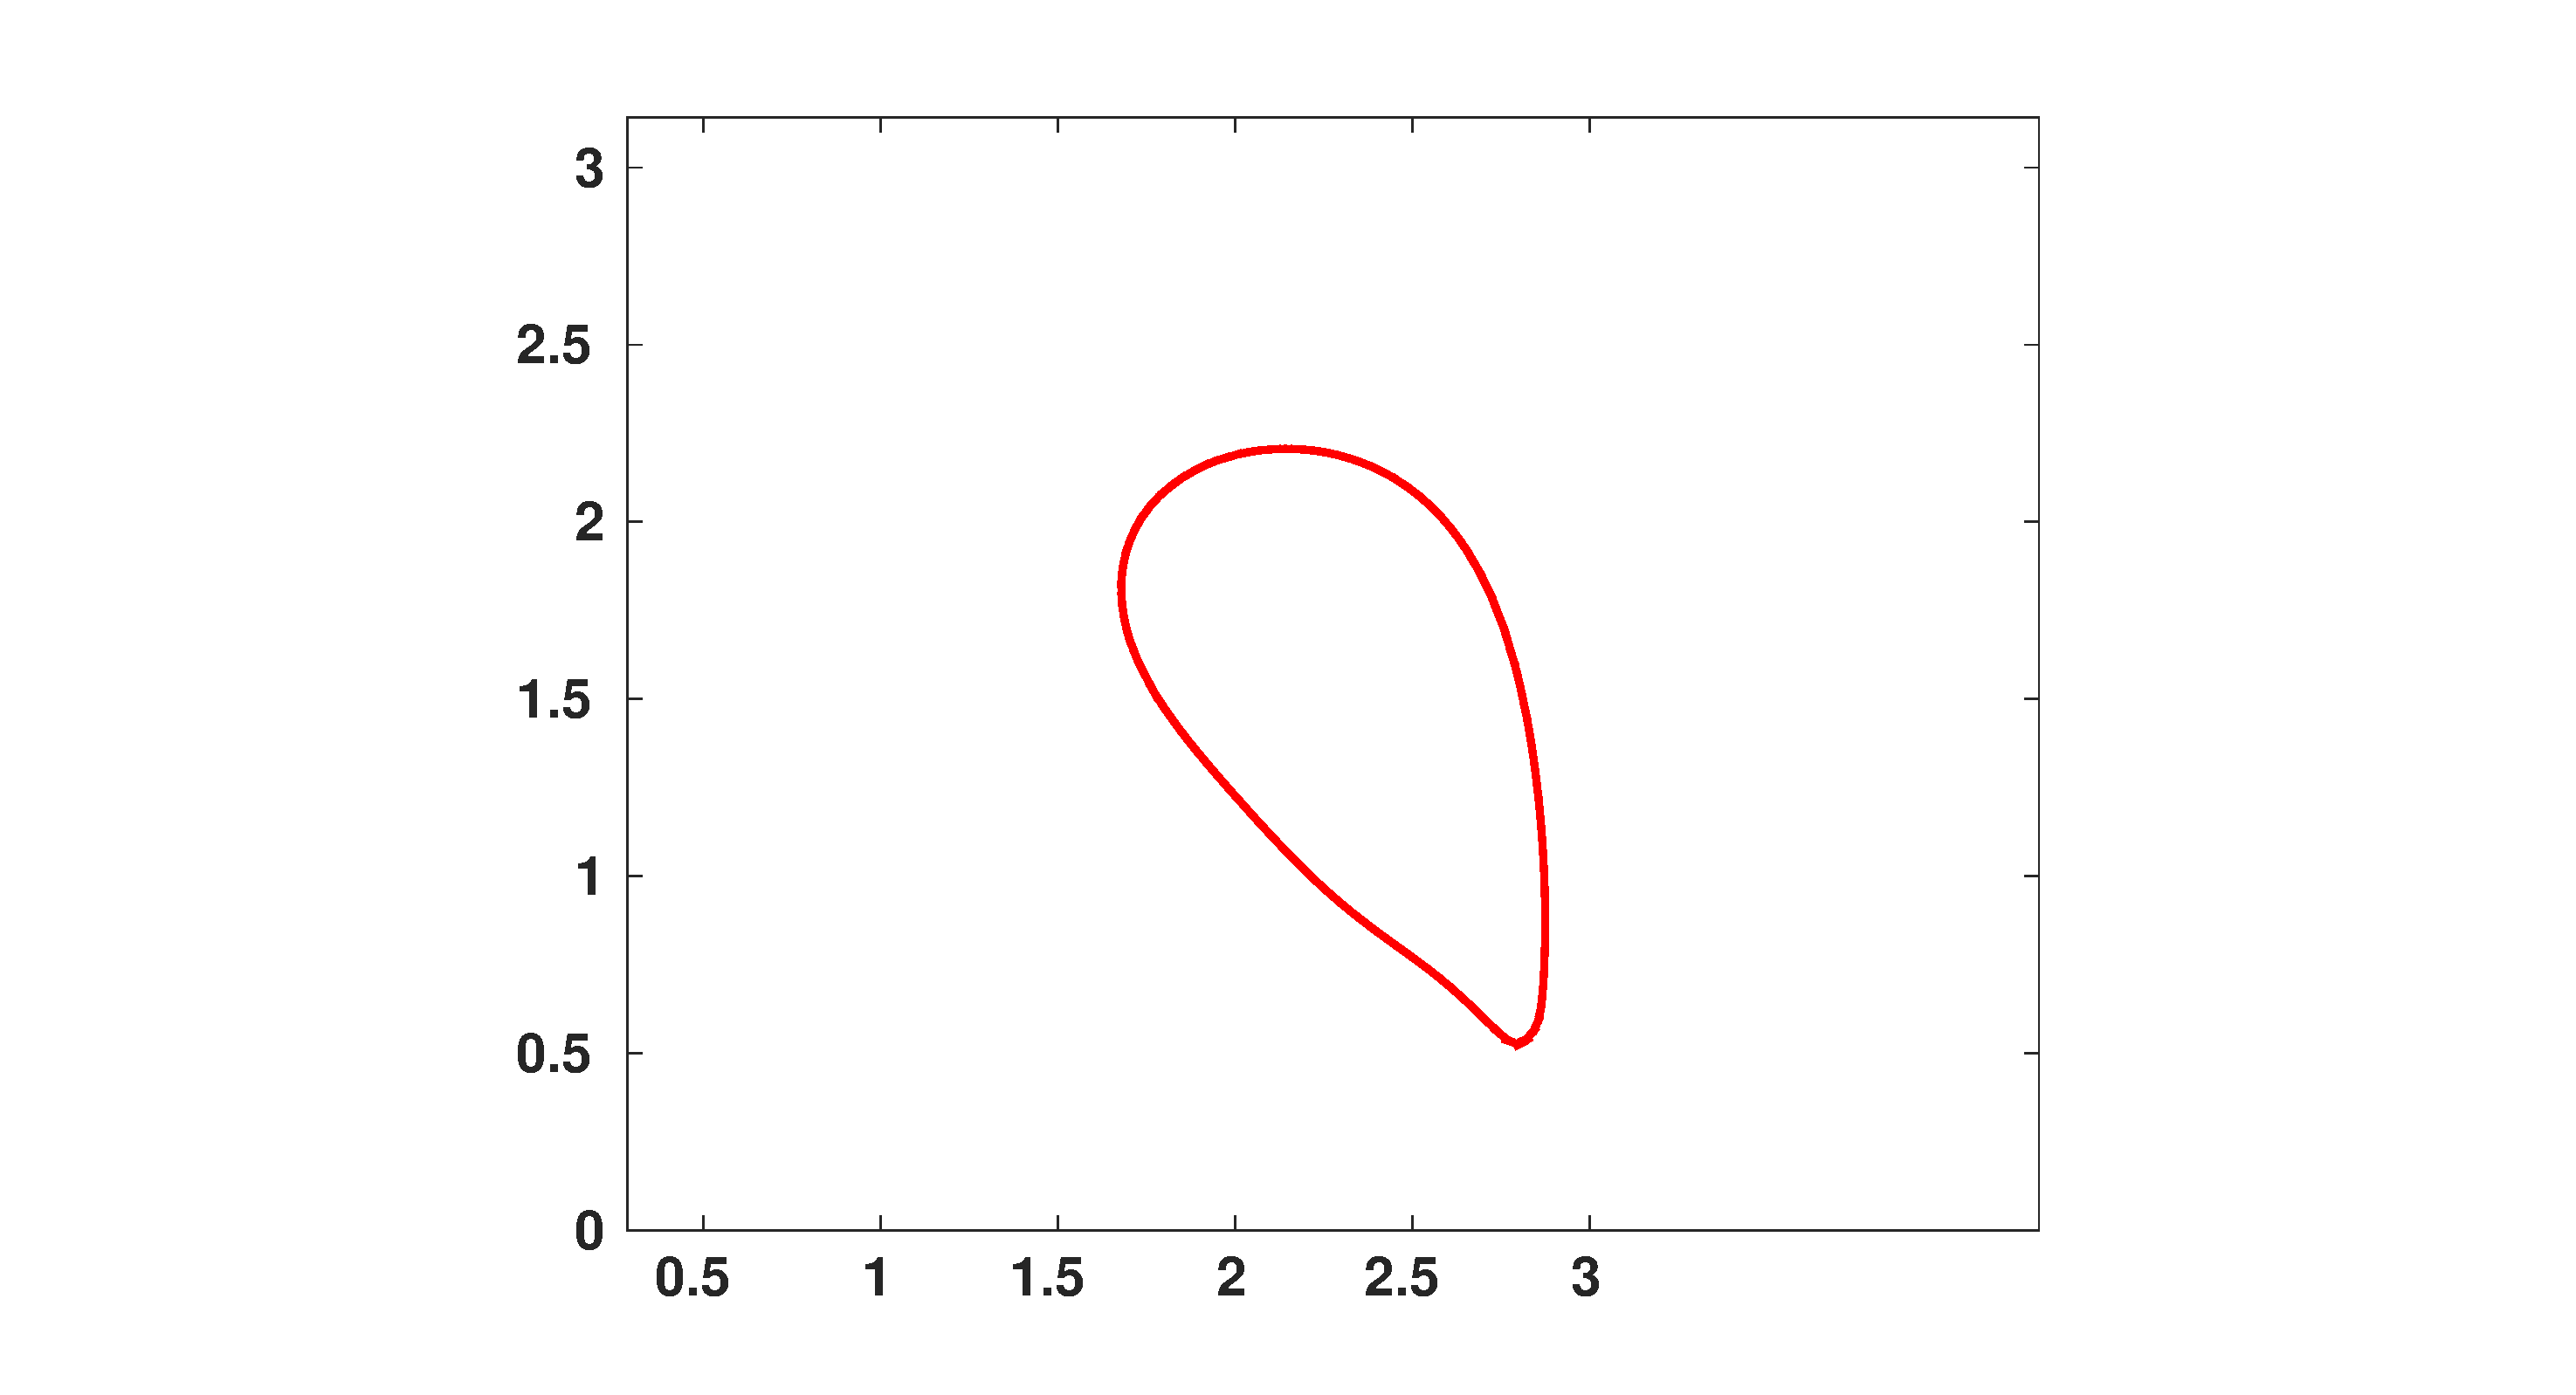
\includegraphics[width=0.5\textwidth]{shear_250.eps}
      } \\
      \subfloat[After advecting 500 steps ]{%
      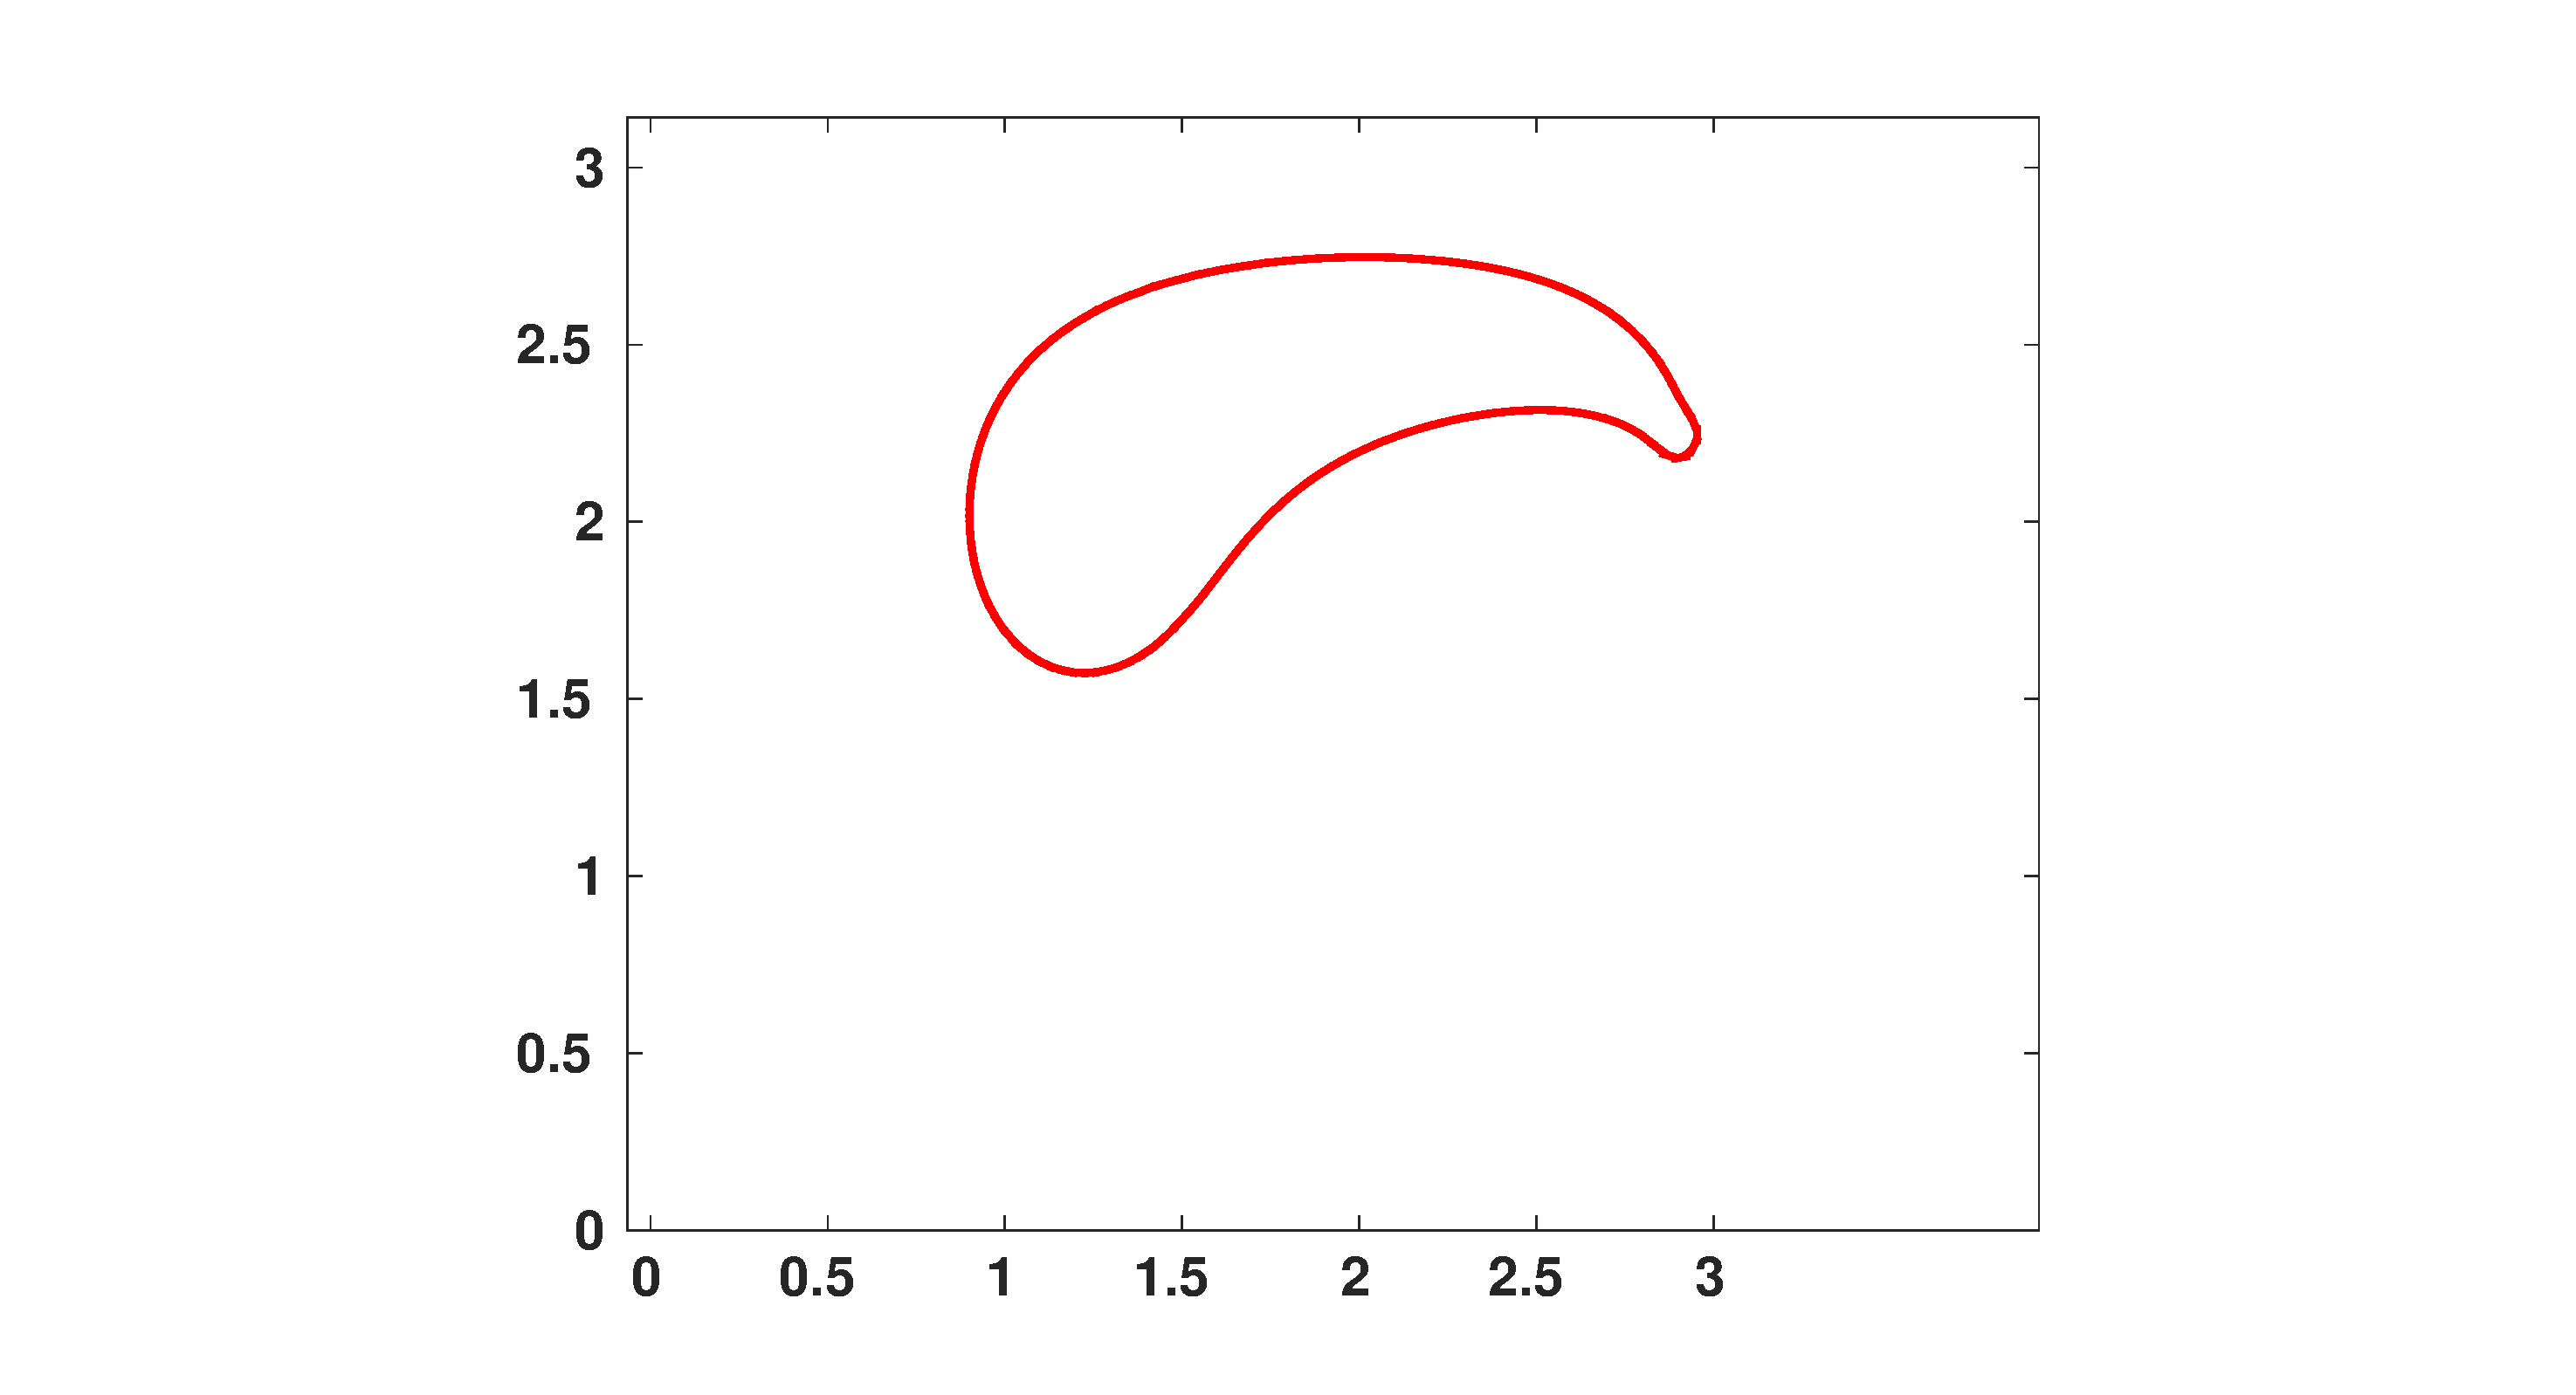
\includegraphics[width=0.5\textwidth]{shear_500.eps}
      }
      \subfloat[After advecting 1000 steps ]{%
      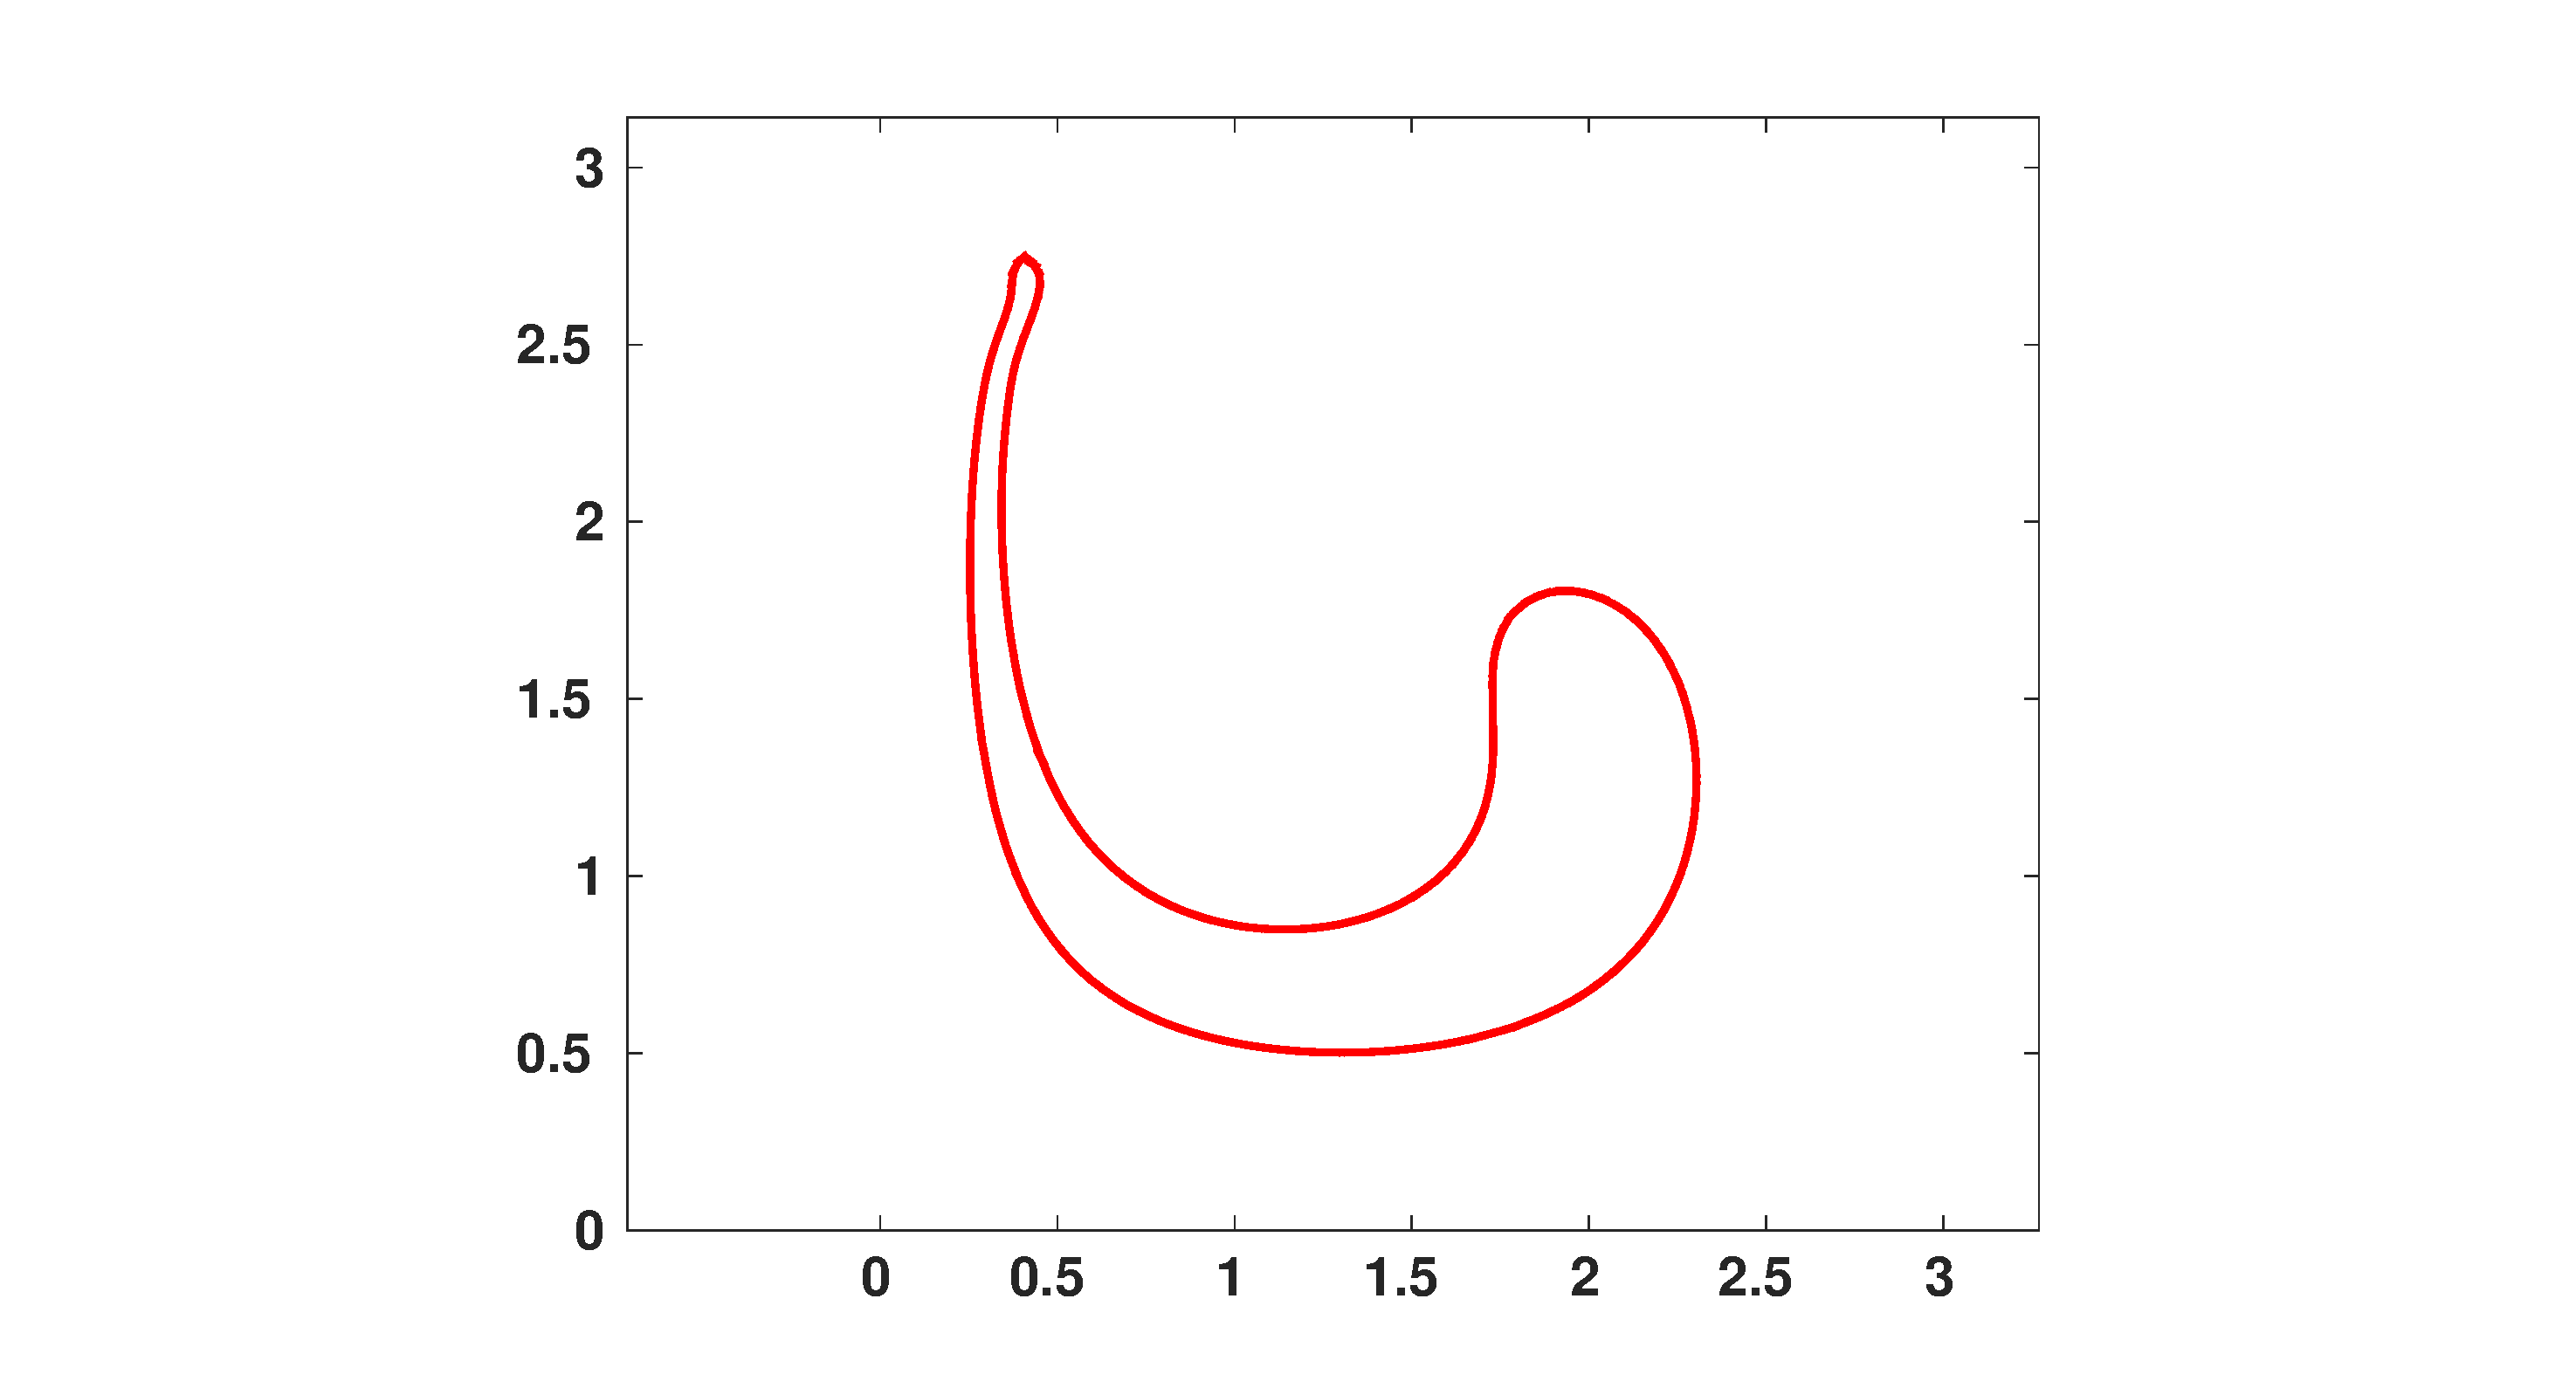
\includegraphics[width=0.5\textwidth]{shear_1000.eps}
      }
 \caption{Advection test result for shear velocity field}
 \label{Fig:shear}
\end{figure}

\begin{figure}
 \centering
 \subfloat[After 1000 steps forward ]{%
      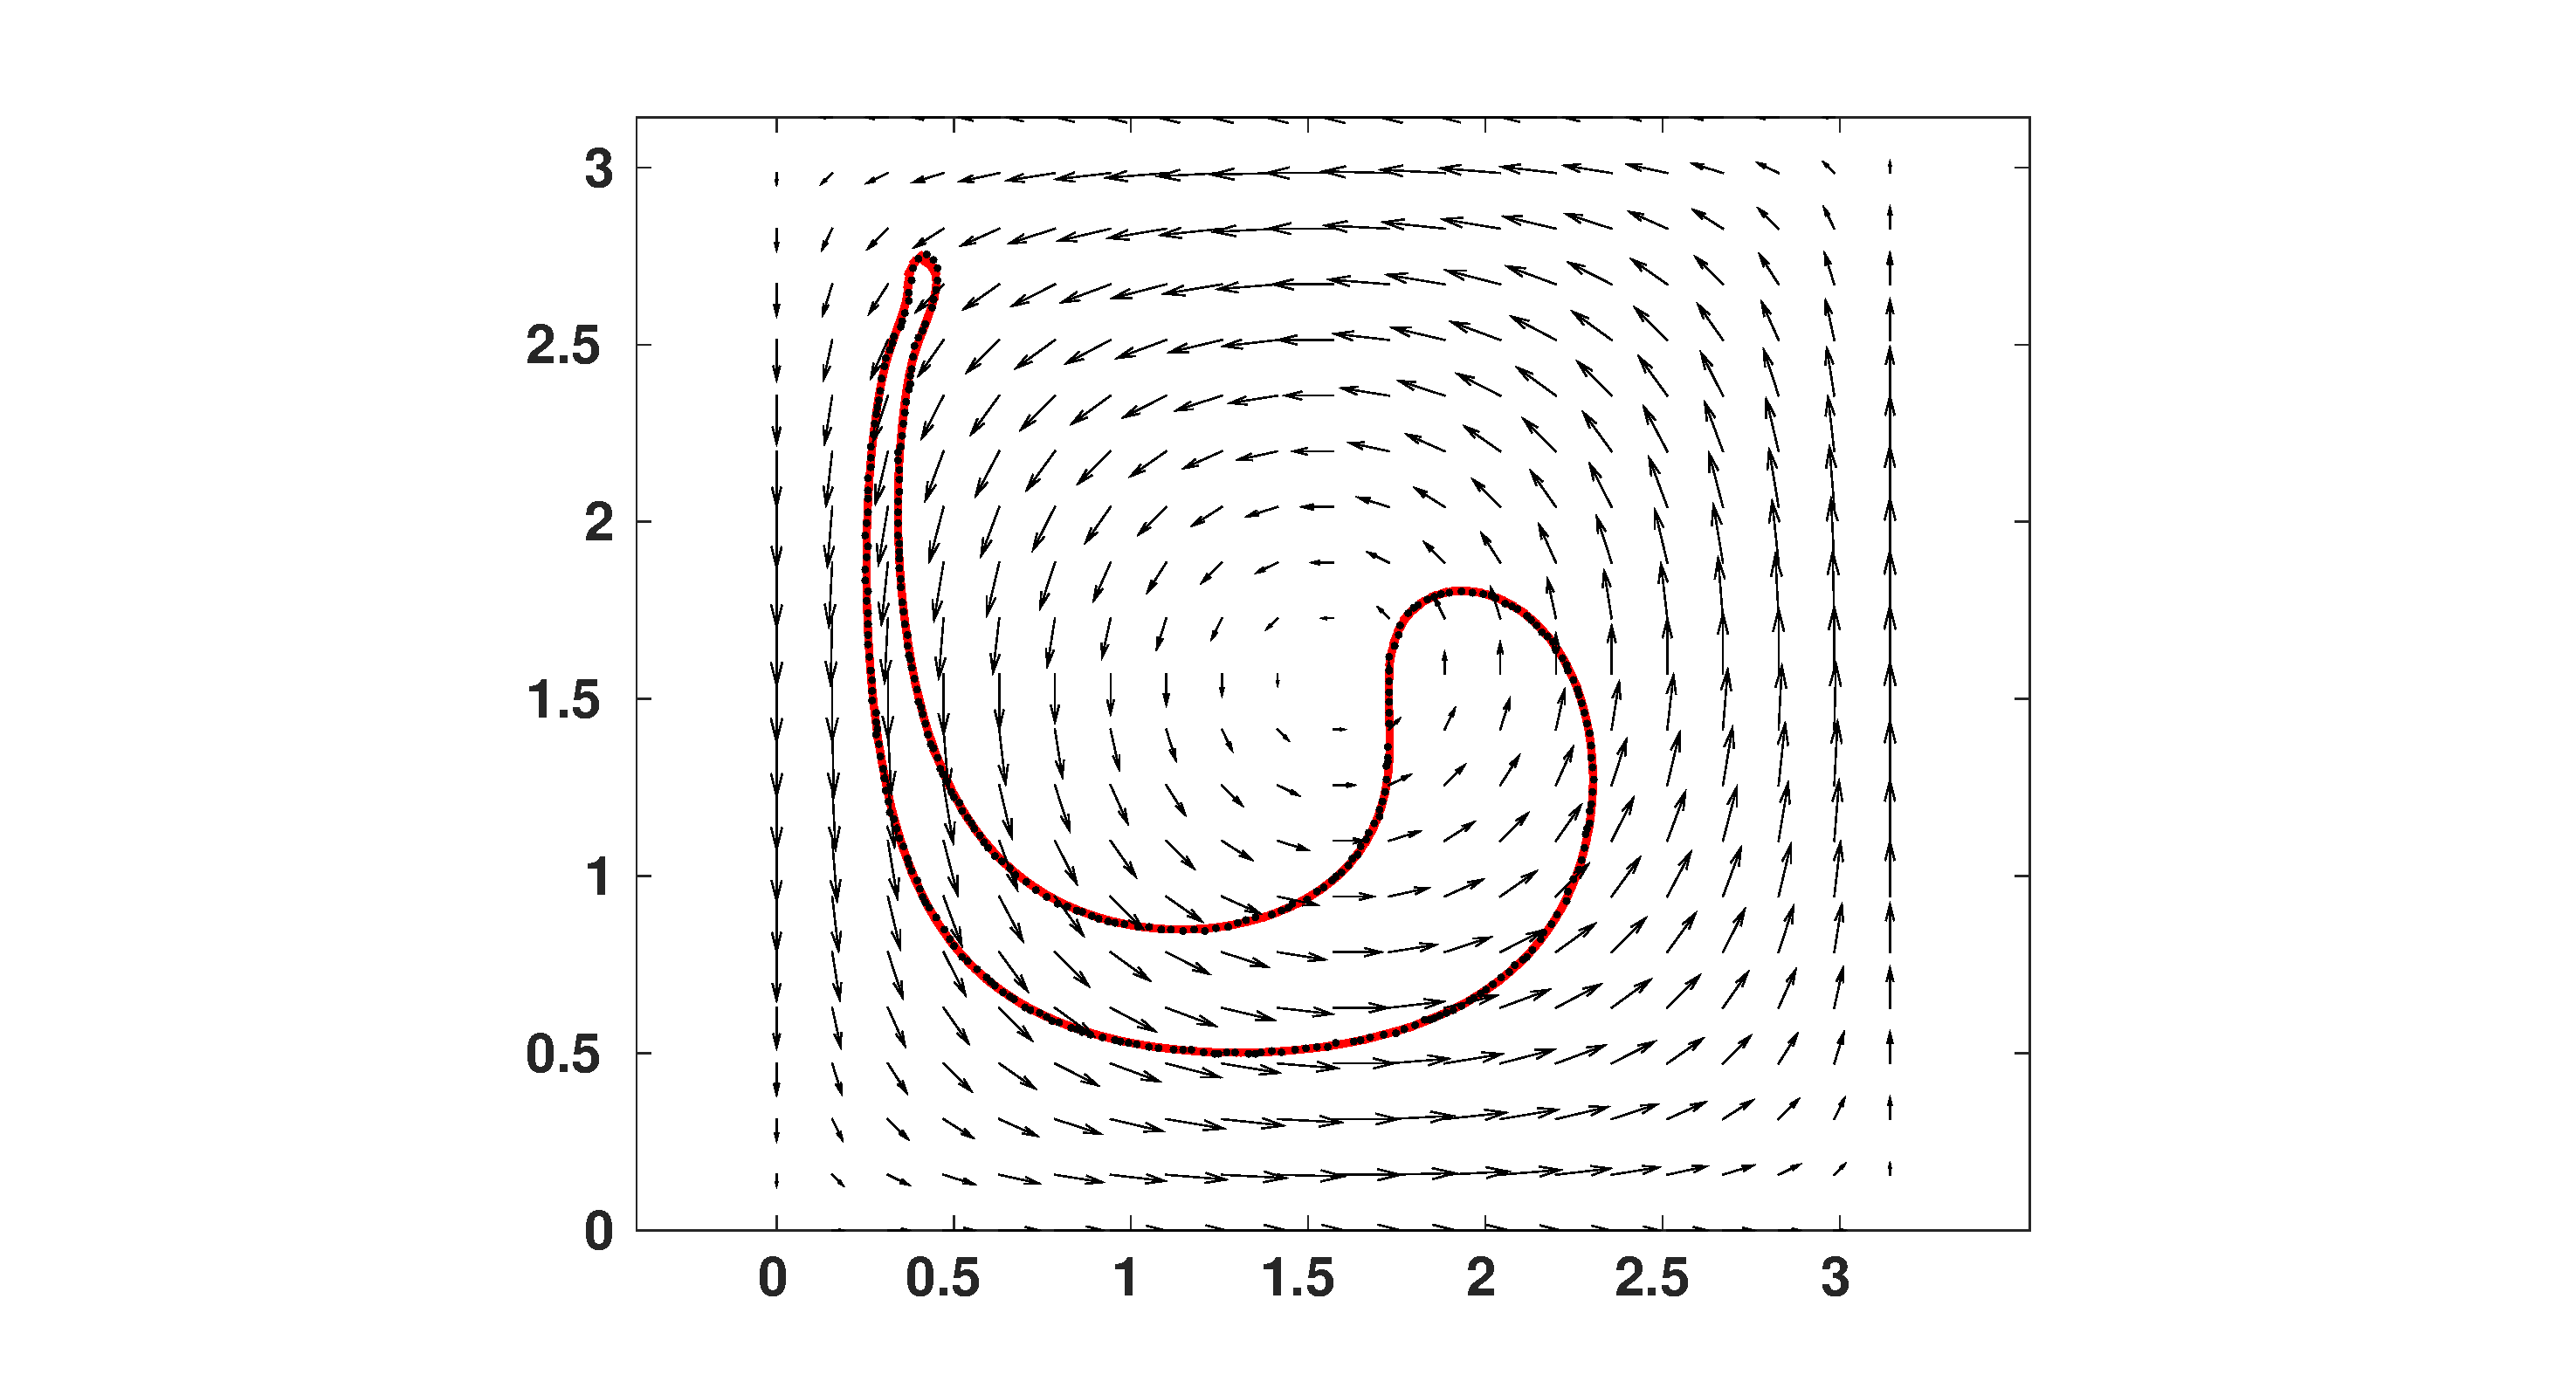
\includegraphics[width=0.5\textwidth]{shear_1000c.eps}
      }
  \subfloat[1000 steps backward followed by 1000 steps forward ]{%
      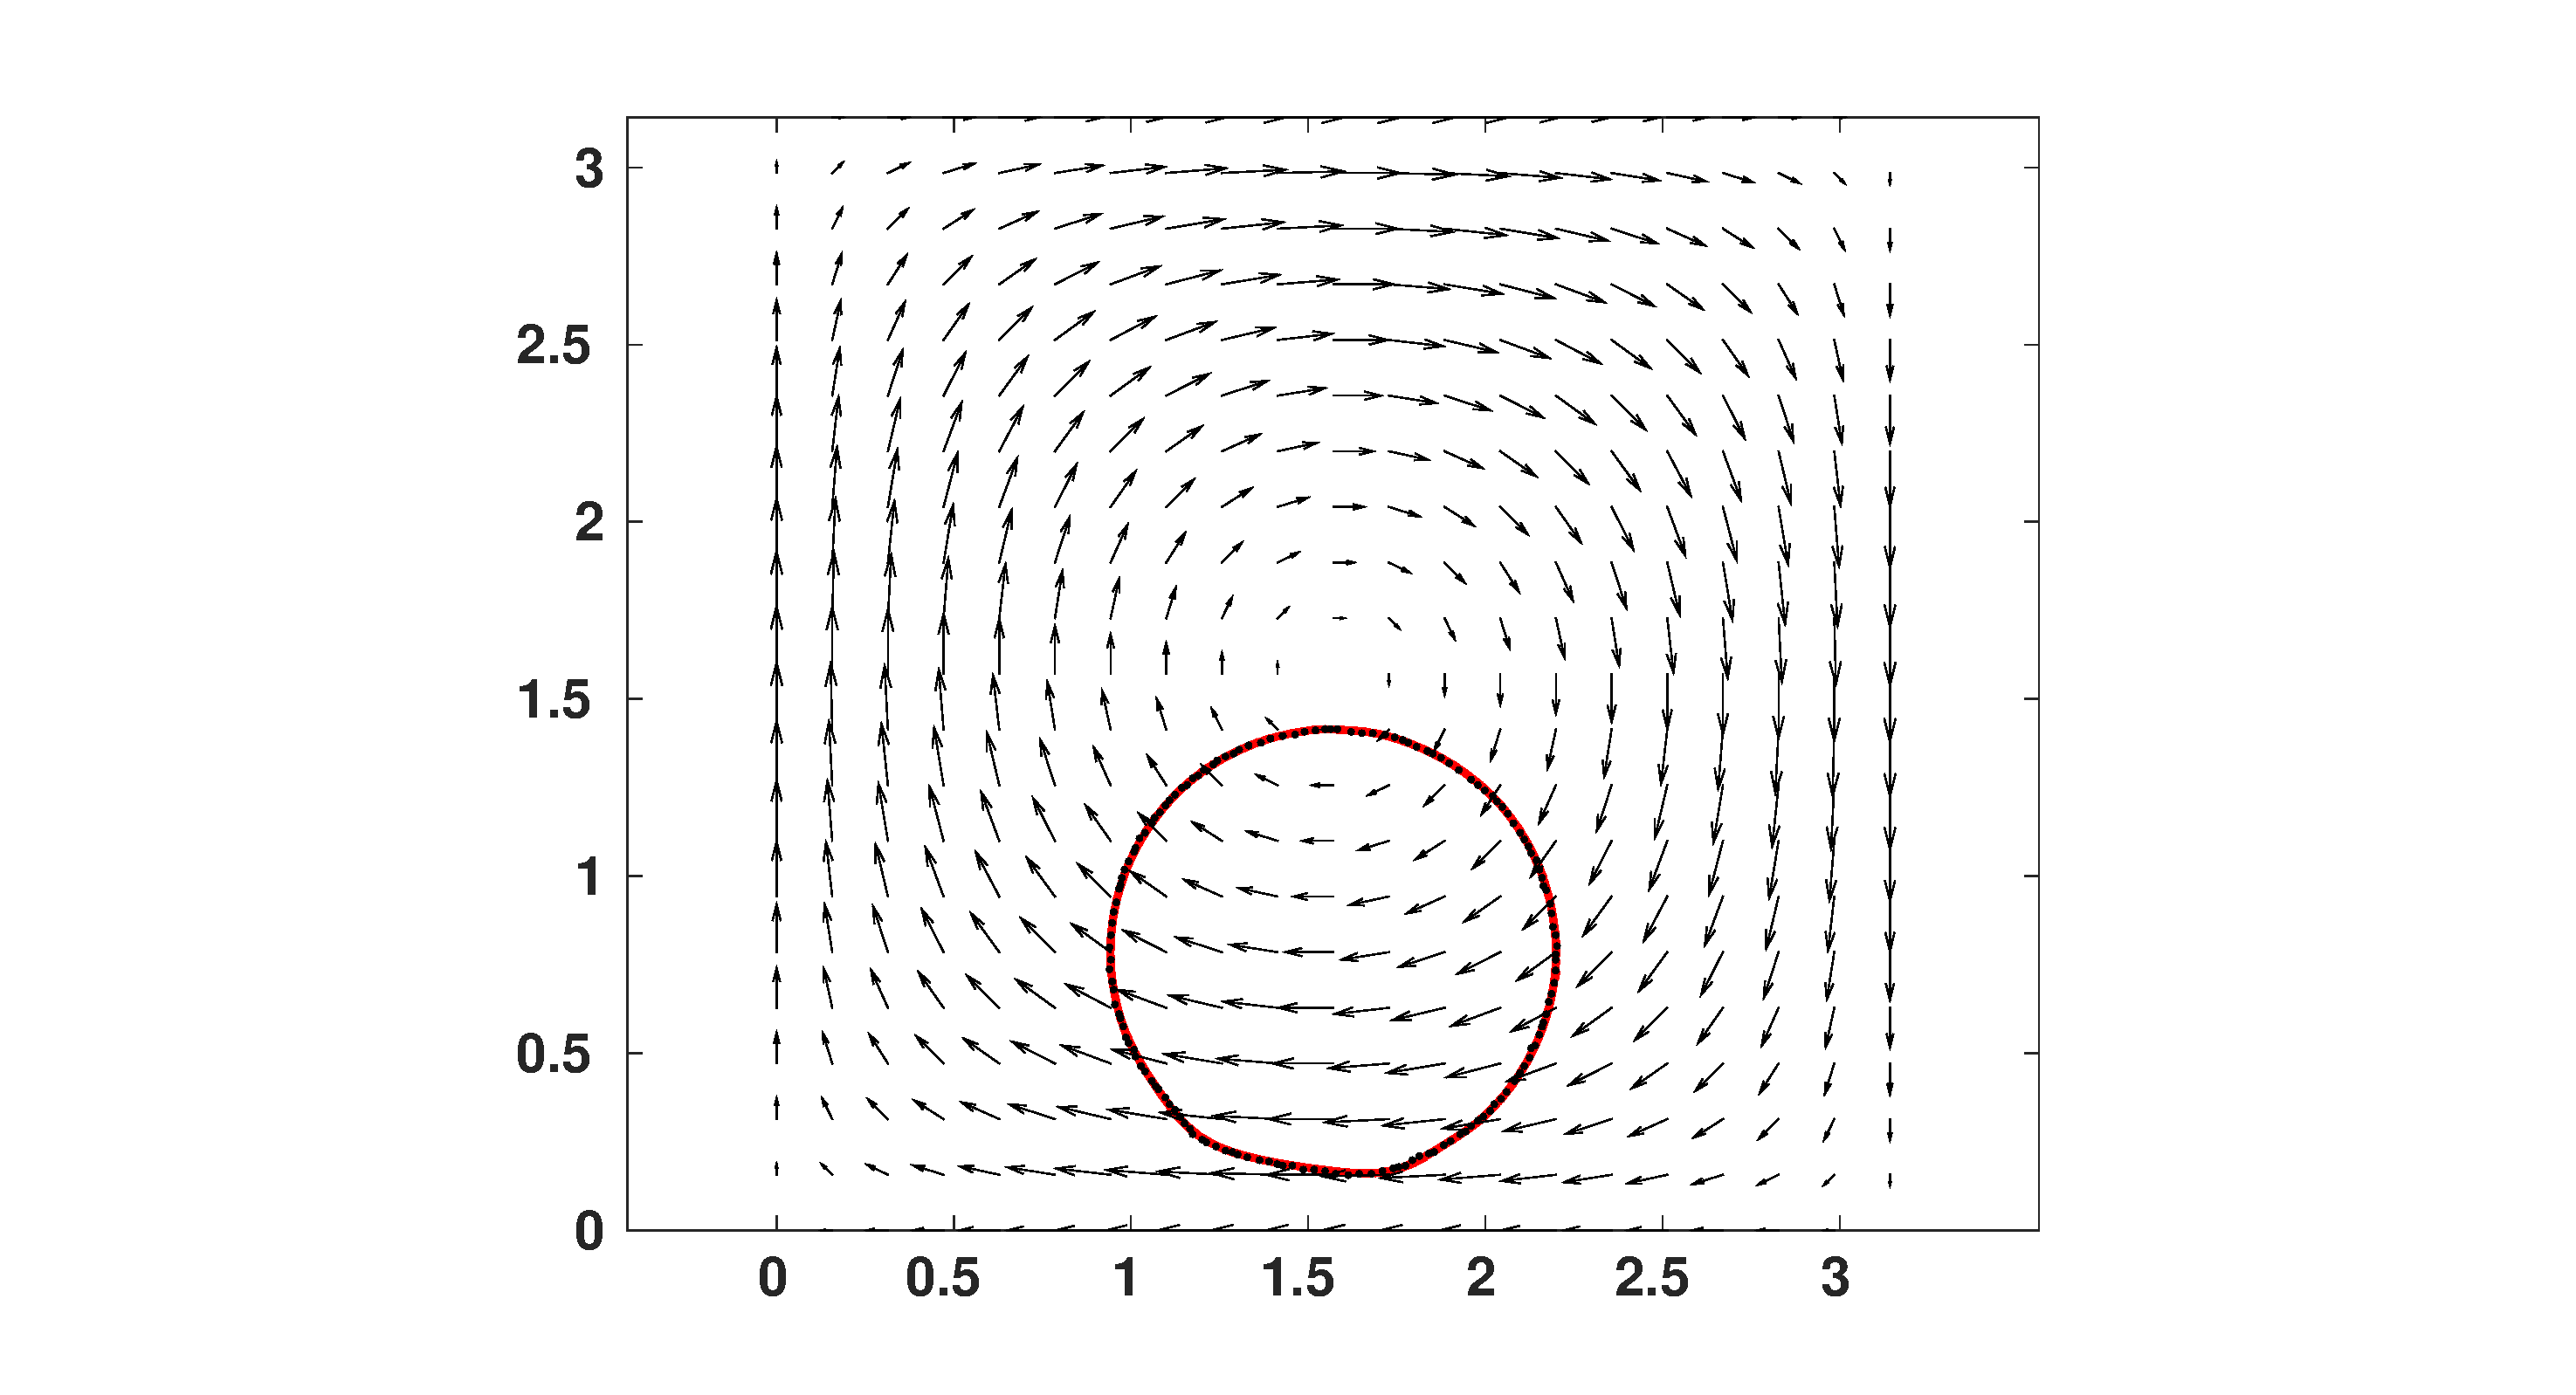
\includegraphics[width=0.5\textwidth]{shear_back.eps}
      }
 \caption{Comparison with \cite{Gerlach2006} results. (Red LVIRA and Blue \cite{Gerlach2006} data)}
 \label{Fig:shear_comparison}
\end{figure}

\subsection{Calculation of error}

The above results can be quantified by defining the error as
\begin{equation}
 E = \frac{\sum |{F^n_{r,c}-F^e_{r,c}}|}{\sum F^0_{r,c}}
\end{equation}
where E is the ratio of summation of difference between the volume fraction of cells of calculated solution and exact solution to the total sum inital volume fraction over all the cells.
where $F^n$ is the solution of volume fraction field after n time steps of computation, $F^e$ is the exact solution, and $F^0$ is the initial solution. The initial solution can be calculated by the initial 
volume fraction field, exact solution of field for translational velocity fields can be easily calculated by recreating the circle at the center which has moved with the velocity field. For solid body
rotation the exact solution is equal to the initial solution after one full rotation. For the shear test after 1000 backward steps the final solution should also be equal to initial solution.
The errors calculated for various tests are shown in Table \ref{Table:errors} and compared with \cite{Rudman1997}.

\begin{table}
  \begin{center}
    \caption{Errors for various tests}
 \label{Table:errors}
    \begin{tabular}{p{3cm}llll|a}
      \toprule 
       Test & SLIC & Hirt-Nichols & FCT-VOF & Youngs & LVIRA (Present Study)  \\ 
      \midrule
      Translational (V(1,0)) & $1.30 X 10^{-2}$ & $4.55 X 10^{-2}$ & $1.28 X 10^{-2}$ & $3.08 X 10^{-3}$ & $1.5 X 10^{-3}$  \\ 
        Translational (V(2,1)) & $9.18 X 10^{-2}$ & $1.9 X 10^{-1}$ & $3.99 X 10^{-2}$ & $2.98 X 10^{-2}$ & $1.05 X 10^{-2}$  \\ 
      Shear Flow & $4.59 X 10^{-2}$ & $6.66 X 10^{-2}$ & $3.14 X 10^{-2}$ & $8.60 X 10^{-3}$ & $6.90 X 10^{-3}$  \\ 
       Solid Body Rotation (Slotted circle) & $8.38 X 10^{-2}$ & $9.62 X 10^{-2}$ & $3.29 X 10^{-2}$ & $1.09 X 10^{-2}$ & $9.7 X 10^{-3}$  \\ 
        
      \bottomrule \\
    \end{tabular}
  \end{center}
\end{table}


\section{Conclusion}
The reconstruction and advection of an interface is calculated mostly geometrical techniques and does not require extensive knowledge of computational techniques. We found LVIRA
is more accurate than other methods available in the literature. We will couple this algorithm with a flow solver which we have discussed in the next chapter. 
%
\chapter{Superhydrophobic Droplet Impact - Comparison with Gerris simulations}

\section{Contact angle}
\begin{wrapfigure}{r}{0.5\textwidth}
  \begin{center}
    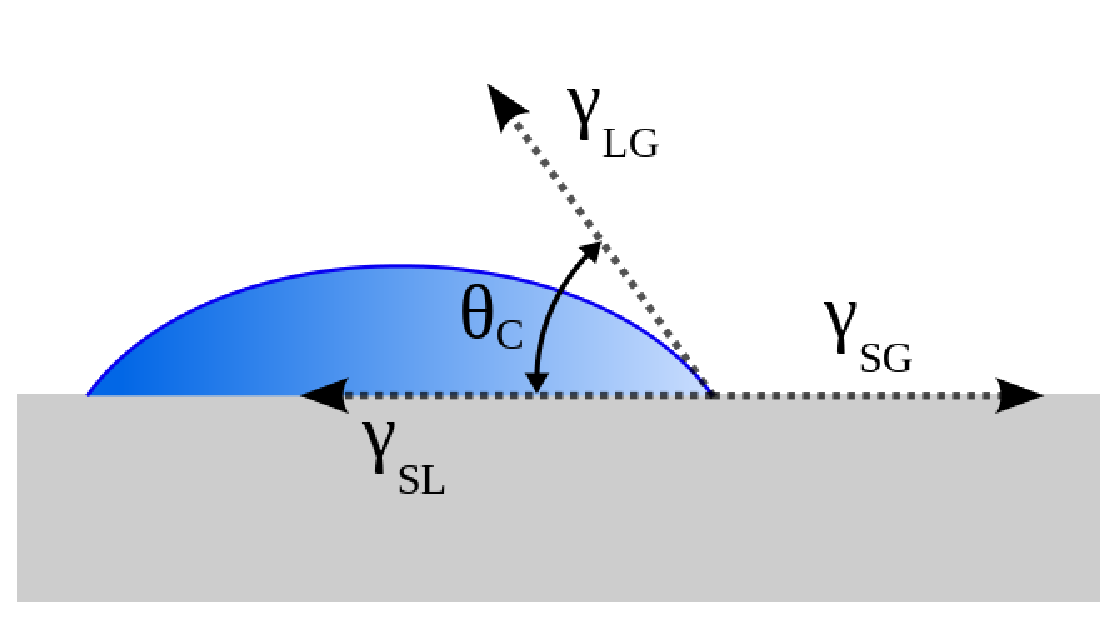
\includegraphics[width=0.48\textwidth]{Contact_angle.eps}
  \end{center}
  \caption{Contact Angle}
  \label{Fig:Contact_angle}
\end{wrapfigure}
When a gas-liquid interface meets a solid surface, at the point of contact of three phases the liquid makes an angle with the surface. This measures the wettability of 
the solid surface for that liquid. The contact angle is given by Youngs equation, ( See Figure \ref{Fig:Contact_angle} ). 
\begin{equation}
 \boxed{ \begin{align}
 &\gamma_{SG} -\gamma_{SL} - \gamma_{LG} \cos \theta =0  \\
 &\cos \theta =\frac{\gamma_{SG} -\gamma_{SL}}{\gamma_{LG}} 
 \end{align}
 }
 \label{Eq:youngs}
\end{equation}
which expresses the balance of forces acting on the contact line in the direction normal to the contact line and tangential
to the solid surface. Experiments show that the contact angle deviates from its static value when
the contact line is in motion.This deviation is an important feature of the problem and needs to be taken into account to obtain realistic answers. \\
\\
\underline{\textbf{Superhydrophobic surfaces}}\\
The effect of the dynamic contact angle and moving contact line however can be made minimal if the spreading of the droplet is very less. Such phenomenon is seen in non-wetting surfaces. 
Surfaces which are extremely difficult to wet are known as superhydrophobic surfaces. \cite{wang2007definition} has attempted to define the superhydrophobic surfaces as the
surfaces that exhibit static contact angle greater than $150^o$. In the next sections we compared some experimental studies on superhydrophobic surfaces with simulations done on Gerris.
% \begin{figure}
% \centering
%     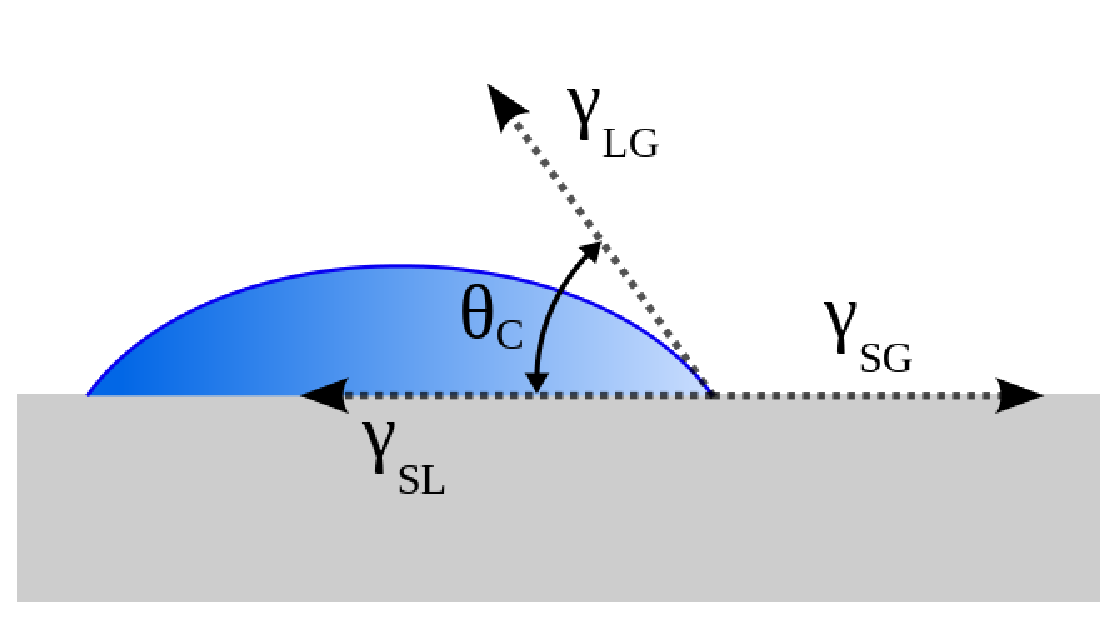
\includegraphics[width=0.48\textwidth]{Contact_angle.eps}
%   \caption{Contact angle}
%   \label{Fig:Contact_angle}
% \end{figure}

\section{Gerris}
Gerris is an open source code created by \cite{Popinet2003} which solves Navier stokes equation using a VOF method for constructing the interface.
However the units are non-dimensional, we can use any system of units, it have to be consistent throughout
the simulation file and the results will be in those units.

\begin{equation}
 \boxed{ \begin{align}
 \frac{d \overrightarrow u}{dt} &= \frac{1}{\rho} \left\{ - \overrightarrow \nabla p + \overrightarrow \nabla \cdot ( \mu (\overrightarrow \nabla \overrightarrow u + \nabla \overrightarrow u^T )) + \sigma \kappa \delta_s \overrightarrow n \right\} + { {\tt Source} }(\overrightarrow u)\\
 \overrightarrow \nabla . \overrightarrow u &= 0 \qquad\text{(Equation of continuity)}\\
\frac{DF}{Dt}&=0 \qquad\text{(Volume of Fluid advection equation)}
\end{align} }
\label{Eq:gerris}
\end{equation}

There are some limitations in Gerris flow solver
\begin{enumerate}
 \item No contact line model
 \item No dynamic contact angle model
\end{enumerate}

To know the effects of these two limitations, we compared the Gerris simulation with \cite{Hung2011}, \cite{Clanet2004} and \cite{Wang2007}
having no-slip conditions and static contact angle at the surface.
\section{Gerris Simulation}
To run simulations in we have to find the non dimensional parameters for our problem.
We use Buckingham $\pi$ method to find out number of non dimensional parameters ( See Table \ref{table:bp} )
\begin{table}
  \begin{center}
    \caption{Dimensional matrix to determine non-dimensional groups}
    \label{table:bp}
      \begin{tabular}{c c c c c c c c c c}
	\toprule
	Dimensional Variables & $\rho_L$ & $\rho_g$ & $\mu_L$ & $\mu_g$ & $\sigma_{Lg}$ & $L_b$ & $D_o$ & $H_o$ & $g$ \\
	\midrule
	M & 1 & 1 & 1 & 1 & 1 & 0 & 0 & 0 & 0 \\
	L & -3 & -3 & -1 & -1 & 0 & 1 & 1 & 1 & 1 \\
	T & 0 & 0 & -1 & -1& -2 & 0 & 0 & 0 & -2 \\
	\bottomrule
      \end{tabular}
     \end{center}
 \end{table}

Rank of the matrix = 3 \\

Number of independent non-dimensional parameters = 9-3 = 6 \\

Gerris simulation takes a dimensional input as parameters for density, viscosity of both fluids, surface tension and source term (generally gravitational acceleration. 
We can non-dimensionalise the equation \ref{Eq:gerris} which Gerris solves. We choose scales as characteristic length  L, characteristic velocity U,
characteristic time $\frac{L}{U}$, characteristic pressure $\rho_L U^2$, characteristic density $\rho_L$ and characteristic viscosity $\mu_L$.
Substitute $u = U\tilde u $, $x = L\tilde x $, $y = L\tilde y $, $t = \frac{L}{U}\tilde t $, $p = \rho_L U^2\tilde p $, $\rho = \rho_L \tilde\rho $, $\mu = \mu_L \tilde\mu $
in \ref{Eq:gerris}, where quantities with tilde are non-dimensional.

\begin{equation}
 \boxed {\begin{align}
 \frac{d \tilde u}{d\tilde t} &= \frac{1}{\rho_k} \left\{ - \tilde \nabla p + \frac{1}{Re_L}  \tilde \nabla \cdot ( \mu_k (\tilde \nabla \tilde u + \nabla \tilde u^T )) 
 + \frac{1}{We} \kappa \delta_s \overrightarrow n \right\} + \frac{1}{Fr^2} \\
 \tilde \nabla . \tilde u &= 0 \qquad\text{(Equation of continuity)}\\
 \frac{D\tilde F}{D\tilde t}&=0 \qquad\text{(Volume of Fluid advection equation)}
\end{align} }
\label{Eq:gerris_nd}
\end{equation}
where, $Re_L = \frac{L\rho_L U}{\mu_L}$ and $Fr = \frac{U}{\sqrt{gL}}$. \\

\underline{Domain} \\
The domain consists of three boxes and axis of symmetry lies on y-axis ( See Figure \ref{Fig:domain-gerris}), 
\begin{figure}[tbp]
\centering
 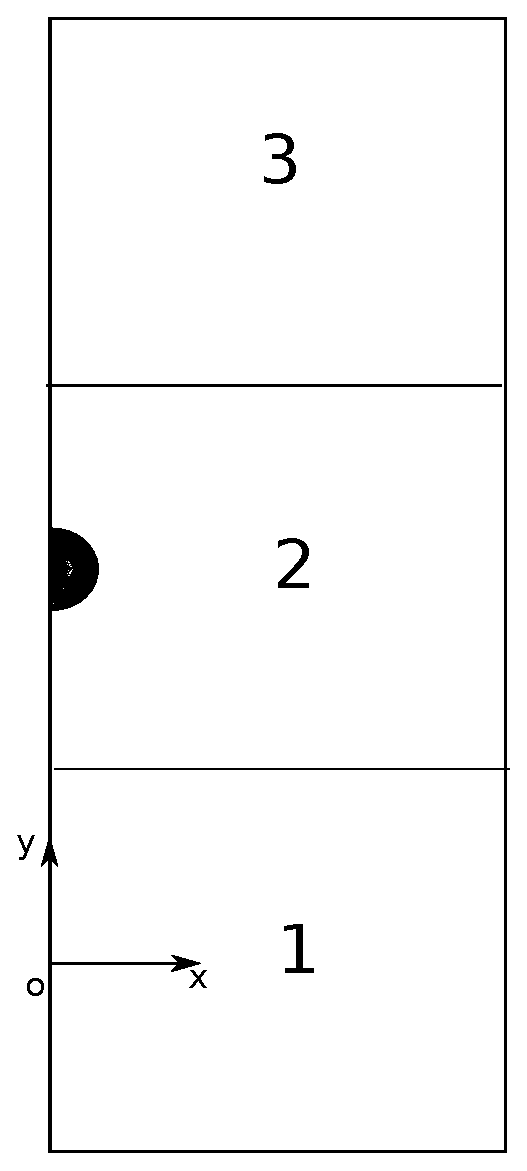
\includegraphics[scale = 0.5]{domain.eps}
 \caption{Domain for simulation (Axisymmetric)}
 \label{Fig:domain-gerris}
\end{figure}

 \begin{table}
  \begin{center}
   \caption{Input for non-dimensional simulation (Calculated from dimensional parameters as in \cite{Hung2011})}
 \label{Table:input}
    \begin{tabular}{lll}
      \toprule 
      Parameter & Remark & Value  \\ 
      \midrule
	Re & Reynolds number & 2521.285386 \\
	We & Weber number of Liquid-gas & 29.43 \\
	$H_k$ & $\frac{H_o}{D_o}$ &  12.00\\
	$L_k$ & $\frac{L_o}{D_o}$ &  2 \\
	$\rho_k$ & $\frac{\rho_g}{\rho_L}$ & $2 X 10^{-3}$  \\ 
	$\mu_k$ & $\frac{\mu_g}{\mu_L}$ & $2 X 10^{-2}$ \\
      
      \bottomrule \\
    \end{tabular}
  \end{center}
\end{table}

\underline{Initial Condition} \\
\begin{equation}
 x^2+(y+(H_k-0.5L_k))^2=0.25  %this equation is altered here from simulation there the axes are inverted
\end{equation}

\underline{Boundary Conditions}: No slip conditions on all walls except axis of symmetry where we use symmetry conditions(described in section \ref{sec:bc}). Impact surface
has a static contact angle of $150^o$.

\section{Results and Discussion}
\begin{figure}[H]
 \centering
 \subfloat[t = 0.0357 ]{%
      \includegraphics[width=0.3\textwidth]{hung-1.eps}
      }
  \subfloat[t = 0.0361 ]{%
      \includegraphics[width=0.3\textwidth]{hung-2.eps}
      } \\
       \subfloat[t = 0.0362 ]{%
      \includegraphics[width=0.3\textwidth]{hung-3.eps}
      }
       \subfloat[t = 0.0365 ]{%
      \includegraphics[width=0.3\textwidth]{hung-4.eps}
      }\\
    \subfloat[t = 0.0368 ]{%
      \includegraphics[width=0.3\textwidth]{hung-5.eps}
      }
       \subfloat[t = 0.0371 ]{%
      \includegraphics[width=0.3\textwidth]{hung-6.eps}
      }\\
       \subfloat[t = 0.0374 ]{%
      \includegraphics[width=0.3\textwidth]{hung-7.eps}
      }
       \subfloat[t = 0.0377 ]{%
      \includegraphics[width=0.3\textwidth]{hung-8.eps}
      }\\
       \subfloat[t = 0.0379 ]{%
      \includegraphics[width=0.3\textwidth]{hung-9.eps}
      }
       \subfloat[t = 0.0382 ]{%
      \includegraphics[width=0.3\textwidth]{hung-10.eps}
      }
 \caption{Interface and center of mass Gerris simulation data(BLUE) with \cite{Hung2011} experimental data(RED), Contact Angle $150^o$}
 \label{Fig:gs5}
 \end{figure}
 
 \begin{figure}[H]
 \includegraphics{y_com_hung.eps}
 \caption{y coordinate of center of mass of droplet to time}
 \label{Fig:y_com}
\end{figure}

The interface points and center of mass from the experimental data(\cite{Hung2011}) were extracted and compared with Gerris simulation data. 
The simulation results were in agreement with experiment before the impact. Just after the impact (See Figure \ref{Fig:gs5} (a),(b)) the contact line and the contact angle is coinciding with 
the experimental but as the contact line started to move in the (c) \& (d), the simulation interface did not moved because of the no slip boundary condition and also has the contact 
contact angle. From (c) to (j) the results are very different from what is observed in the experiment. The vertical position of center of mass is less sensitive to the impact surface.
Figure \ref{Fig:y_com} shows the variation of vertical height of center of mass of droplet with respect to time. It looks like a damped oscillation.  

\begin{figure}[H]
 \centering
 \subfloat[t = 26.2 ]{%
      \includegraphics[width=0.3\textwidth]{clanet-1.eps}
      }
  \subfloat[t = 27.1 ]{%
      \includegraphics[width=0.3\textwidth]{clanet-2.eps}
      } 
       \subfloat[t = 28.0 ]{%
      \includegraphics[width=0.3\textwidth]{clanet-3.eps}
      }\\
       \subfloat[t = 28.9 ]{%
      \includegraphics[width=0.3\textwidth]{clanet-4.eps}
      }
    \subfloat[t = 29.8 ]{%
      \includegraphics[width=0.3\textwidth]{clanet-5.eps}
      }
       \subfloat[t = 30.7 ]{%
      \includegraphics[width=0.3\textwidth]{clanet-6.eps}
      }\\
       \subfloat[t = 31.6 ]{%
      \includegraphics[width=0.3\textwidth]{clanet-7.eps}
      }
       \subfloat[t = 32.5 ]{%
      \includegraphics[width=0.3\textwidth]{clanet-8.eps}
      }
       \subfloat[t = 33.4 ]{%
      \includegraphics[width=0.3\textwidth]{clanet-9.eps}
      }
 \caption{Interface Gerris simulation data(BLUE) with \cite{Clanet2004} experimental data(RED) Contact Angle $170^o$}
 \label{Fig:gs6}
 \end{figure}
 \cite{Clanet2004}  also shown that droplet impacting on superhydrophobic behaves like a balloon filled with fluid in some region of parameters,
 where the movement of contact line is restricted and the boundary condition for velocity can be taken as no-slip. 
 \cite{Clanet2004} study involved superhydrophobic surfaces and with contact angle of  $170^o$. We made a comparison with Gerris simulation with static contact angle
 boundary condition and no slip  at surface (See Figure \ref{Fig:gs6}). It can be seen that superhydrophobic surfaces has minimum spreading and has minimal effect on 
 the dynamics of droplet impact.
 
 \begin{figure}[H]
 \centering
 \subfloat[t = 15.6 ]{%
      \includegraphics[width=0.3\textwidth]{wang-1.eps}
      }
  \subfloat[t = 16.0 ]{%
      \includegraphics[width=0.3\textwidth]{wang-2.eps}
      } 
       \subfloat[t = 17.0 ]{%
      \includegraphics[width=0.3\textwidth]{wang-3.eps}
      }\\
       \subfloat[t = 18.1 ]{%
      \includegraphics[width=0.3\textwidth]{wang-4.eps}
      }
    \subfloat[t = 19.0 ]{%
      \includegraphics[width=0.3\textwidth]{wang-5.eps}
      }
       \subfloat[t = 19.5 ]{%
      \includegraphics[width=0.3\textwidth]{wang-6.eps}
      }
    \caption{Interface Gerris simulation data(BLUE) with \cite{Wang2007} experimental data(RED) Contact Angle $163^o$ }
 \label{Fig:gs7}
 \end{figure}   
  \begin{figure}[H]
 \centering
 \subfloat[t = 15.6 ]{%
      \includegraphics[width=0.3\textwidth]{wang-140-1.eps}
      }
  \subfloat[t = 16.6 ]{%
      \includegraphics[width=0.3\textwidth]{wang-140-2.eps}
      } 
       \subfloat[t = 17.5 ]{%
      \includegraphics[width=0.3\textwidth]{wang-140-3.eps}
      }\\
       \subfloat[t = 20.4 ]{%
      \includegraphics[width=0.3\textwidth]{wang-140-4.eps}
      }
    \subfloat[t = 21.9 ]{%
      \includegraphics[width=0.3\textwidth]{wang-140-5.eps}
      }
       \subfloat[t = 24.6 ]{%
      \includegraphics[width=0.3\textwidth]{wang-140-6.eps}
      }
    \caption{Interface Gerris simulation data(BLUE) with \cite{Wang2007} experimental data(RED) Contact Angle $140^o$}
 \label{Fig:gs8}
 \end{figure}   
A comparison with \cite{Wang2007} (See Figure \ref{Fig:gs7}), the surface has a contact angle of $163^o$, also corroborate the fact that the static contact angle conditions
are a good approximation for the solution of droplet impact on superhydrophobic surfaces.\\
 From above comparisons on superhydrophobic surfaces, we can approximate that the static contact line boundary conditions have negligible effect on droplet impact and we can have
 valid approximations for the dynamics involved.  In the light of above comparisons we want to study some of the problems in superhydrophobic surfaces 
 as below:-  
\begin{enumerate}
\item Motion of center of mass of droplet 
 \item Droplet impact on inclined plane
 \item Droplet impact inclined to the plane
 \item Oscillations of droplet after impact
 \item Droplet breakup after impact
\end{enumerate}

\section{Conclusion}
Due to this limitation of Gerris code, future work involves development of a multiphase Navier-Stokes solver and to implement the moving contact line and dynamic contact line 
model in it. Till then we will use Gerris code to observed some simpler outcomes of droplet impact on superhydrophobic surfaces.
Our code will mimic the actual droplet impact after implementation of the contact models. We will
look to explain some aspects of this phenomena through a simpler mathematical model.


% \begin{figure}
%  \centering
%  \subfloat[ ]{%
%       \includegraphics[width=0.3\textwidth]{droplet_c1.eps}
%       }
%   \subfloat[t = 27.1 ]{%
%       \includegraphics[width=0.3\textwidth]{droplet_c2.eps}
%       } 
%        \subfloat[t = 28.0 ]{%
%       \includegraphics[width=0.3\textwidth]{droplet_c3.eps}
%       }
%   \caption{Moving contact line during impact}
%   \label{Fig:contact_line}
%   \end{figure}

%
\chapter{Validation of Volume of fluid algorithm}
Volume of Fluid method is validated by chosing three test cases from \cite{Rudman1997}, 
\begin{enumerate}
 \item Circle in translational flow
 \item Solid body rotation of slotted circle
 \item Circle in shear flow
\end{enumerate}



\section{Errors}
\begin{table}[tbp]
  \begin{center}
    \caption{Error for various tests}
    \label{tab:samtab}
    \begin{tabular}{p{3cm}lllll}
      \toprule 
       Test & SLIC & Hirt-Nichols & FCT-VOF & Youngs & LVIRA  \\ 
      \midrule
      Translational (V(1,0)) & $1.30 X 10^{-2}$ & $4.55 X 10^{-2}$ & $1.28 X 10^{-2}$ & $3.08 X 10^{-3}$ & $1.5 X 10^{-3}$  \\ 
        Translational (V(2,1)) & $9.18 X 10^{-2}$ & $1.9 X 10^{-1}$ & $3.99 X 10^{-2}$ & $2.98 X 10^{-2}$ & $1.05 X 10^{-2}$  \\ 
      Shear Flow & $4.59 X 10^{-2}$ & $6.66 X 10^{-2}$ & $3.14 X 10^{-2}$ & $8.60 X 10^{-3}$ & $6.90 X 10^{-3}$  \\ 
       Solid Body Rotation (Slotted circle) & $8.38 X 10^{-2}$ & $9.62 X 10^{-2}$ & $3.29 X 10^{-2}$ & $1.09 X 10^{-2}$ & $9.7 X 10^{-3}$  \\ 
        
      \bottomrule \\
    \end{tabular}
  \end{center}
\end{table}






%\section{Results and Discussion}
% 
% \section{Dimensional and Non-Dimensional Simulations}
% 
% The problem has a initial condition for interface of the droplet at a height $H_o$ from the bottom of the domain. It can be seen that both dimensional and non-dimensional simulation 
% interface overlaps each other (See Figure \ref{Fig:gs1} and \ref{Fig:gs2}).
% \begin{figure}
% \def\tabularxcolumn#1{m{#1}}
% \begin{tabularx}{\linewidth}{@{}cXX@{}}
% %
% \begin{tabular}{cc}
% \centering
% \subfloat[t = 0]{\includegraphics[scale=0.4]{Hung_D_ND-0.eps}} 
%    & \subfloat[t = 0.01]{\includegraphics[scale=0.4]{Hung_D_ND-0.01.eps}}\\
% \subfloat[t = 0.02]{\includegraphics[scale=0.4]{Hung_D_ND-0.02.eps}} 
%    & \subfloat[t = 0.03]{\includegraphics[scale=0.4]{Hung_D_ND-0.03.eps}}\\
% \subfloat[t = 0.04]{\includegraphics[scale=0.4]{Hung_D_ND-0.04.eps}} 
%    & \subfloat[t = 0.05]{\includegraphics[scale=0.4]{Hung_D_ND-0.05.eps}}\\
%     \subfloat[t = 0.06]{\includegraphics[scale=0.4]{Hung_D_ND-0.06.eps}}
%    & \subfloat[t = 0.07]{\includegraphics[scale=0.4]{Hung_D_ND-0.07.eps}}\\
% \end{tabular}
% \end{tabularx}
% \caption{Comparison of Dimensional(Blue) and Non-Dimensional(Red) simulations in Gerris (t = Dimensional time in seconds)}
% \label{Fig:gs1}
% \end{figure}
% 
% \begin{figure}
% \def\tabularxcolumn#1{m{#1}}
% \begin{tabularx}{\linewidth}{@{}cXX@{}}
% %
% \begin{tabular}{cc}
%   \subfloat[t = 0.08]{\includegraphics[scale=0.4]{Hung_D_ND-0.08.eps}}
%    & \subfloat[t = 0.09]{\includegraphics[scale=0.4]{Hung_D_ND-0.09.eps}}\\
%     \subfloat[t = 0.10]{\includegraphics[scale=0.4]{Hung_D_ND-0.1.eps}}
%    & \subfloat[t = 0.11]{\includegraphics[scale=0.4]{Hung_D_ND-0.11.eps}}\\
%     \subfloat[t = 0.12]{\includegraphics[scale=0.4]{Hung_D_ND-0.12.eps}}
%    & \subfloat[t = 0.13]{\includegraphics[scale=0.4]{Hung_D_ND-0.13.eps}}\\
%     \subfloat[t = 0.14]{\includegraphics[scale=0.4]{Hung_D_ND-0.14.eps}}
%    & \subfloat[t = 0.15]{\includegraphics[scale=0.4]{Hung_D_ND-0.15.eps}}
% \end{tabular}
% \end{tabularx}
% \caption{Comparison of Dimensional(Blue) and Non-Dimensional(Red) simulations in Gerris (t = Dimensional time in seconds)}
% \label{Fig:gs2}
% \end{figure}
% 
% \begin{figure}
% \def\tabularxcolumn#1{m{#1}}
% \begin{tabularx}{\linewidth}{@{}cXX@{}}
% %
% \begin{tabular}{cc}
%   \subfloat[t = 0.16]{\includegraphics[scale=0.4]{Hung_D_ND-0.16.eps}}
%    & \subfloat[t = 0.17]{\includegraphics[scale=0.4]{Hung_D_ND-0.17.eps}}\\
%     \subfloat[t = 0.18]{\includegraphics[scale=0.4]{Hung_D_ND-0.18.eps}}
%    & \subfloat[t = 0.19]{\includegraphics[scale=0.4]{Hung_D_ND-0.19.eps}}\\
%     \subfloat[t = 0.20]{\includegraphics[scale=0.4]{Hung_D_ND-0.2.eps}}
%    & \subfloat[t = 0.21]{\includegraphics[scale=0.4]{Hung_D_ND-0.21.eps}}\\
%     \subfloat[t = 0.22]{\includegraphics[scale=0.4]{Hung_D_ND-0.22.eps}}
%    & \subfloat[t = 0.23]{\includegraphics[scale=0.4]{Hung_D_ND-0.23.eps}}
% \end{tabular}
% \end{tabularx}
% \caption{Comparison of Dimensional(Blue) and Non-Dimensional(Red) simulations in Gerris (t = Dimensional time in seconds)}
% \label{Fig:gs3}
% \end{figure}
% 
% \begin{figure}
% \def\tabularxcolumn#1{m{#1}}
% \begin{tabularx}{\linewidth}{@{}cXX@{}}
% %
% \begin{tabular}{cc}
%   \subfloat[t = 0.24]{\includegraphics[scale=0.4]{Hung_D_ND-0.24.eps}}
%    & \subfloat[t = 0.25]{\includegraphics[scale=0.4]{Hung_D_ND-0.25.eps}}\\
%     \subfloat[t = 0.26]{\includegraphics[scale=0.4]{Hung_D_ND-0.26.eps}}
%    & \subfloat[t = 0.27]{\includegraphics[scale=0.4]{Hung_D_ND-0.27.eps}}\\
%     \subfloat[t = 0.28]{\includegraphics[scale=0.4]{Hung_D_ND-0.28.eps}}
%    & \subfloat[t = 0.29]{\includegraphics[scale=0.4]{Hung_D_ND-0.29.eps}}\\
%     \subfloat[t = 0.30]{\includegraphics[scale=0.4]{Hung_D_ND-0.3.eps}}
%    & \subfloat[t = 0.31]{\includegraphics[scale=0.4]{Hung_D_ND-0.31.eps}}
% \end{tabular}
% \end{tabularx}
% \caption{Comparison of Dimensional(Blue) and Non-Dimensional(Red) simulations in Gerris (t = Dimensional time in seconds)}
% \label{Fig:gs4}
% \end{figure}
\subsection{Comparison of Gerris simulation with experiment}
The interface points and center of mass from the experimental data(\cite{Hung2011}) were extracted and compared with Gerris simulation data. 
The simulation results were in agreement with experiment before the impact. Just after the impact (See Figure \ref{Fig:gs5} (a),(b)) the contact line and the contact angle is coinciding with 
the experimental but as the contact line started to move in the (c) \& (d), the simulation interface did not moved because of the no slip boundary condition and also has the contact 
contact angle. From (c) to (j) the results are very different from what is observed in the experiment. The vertical position of center of mass is less sensitive to the impact surface
as evident 

\begin{figure}
 \centering
 \subfloat[t = 0.0357 ]{%
      \includegraphics[width=0.3\textwidth]{hung-1.eps}
      }
  \subfloat[t = 0.0361 ]{%
      \includegraphics[width=0.3\textwidth]{hung-2.eps}
      } \\
       \subfloat[t = 0.0362 ]{%
      \includegraphics[width=0.3\textwidth]{hung-3.eps}
      }
       \subfloat[t = 0.0365 ]{%
      \includegraphics[width=0.3\textwidth]{hung-4.eps}
      }\\
    \subfloat[t = 0.0368 ]{%
      \includegraphics[width=0.3\textwidth]{hung-5.eps}
      }
       \subfloat[t = 0.0371 ]{%
      \includegraphics[width=0.3\textwidth]{hung-6.eps}
      }\\
       \subfloat[t = 0.0374 ]{%
      \includegraphics[width=0.3\textwidth]{hung-7.eps}
      }
       \subfloat[t = 0.0377 ]{%
      \includegraphics[width=0.3\textwidth]{hung-8.eps}
      }\\
       \subfloat[t = 0.0379 ]{%
      \includegraphics[width=0.3\textwidth]{hung-9.eps}
      }
       \subfloat[t = 0.0382 ]{%
      \includegraphics[width=0.3\textwidth]{hung-10.eps}
      }
 \caption{Interface and center of mass Gerris simulation data(BLUE) with \cite{Hung2011} experimental data(RED)}
 \label{Fig:gs5}
 \end{figure}
 
% 
% \begin{figure}[tpb]
% \centering
%  \includegraphics[scale=0.3]{hung.eps}
%  \caption{Comparison Gerris simulation data(BLUE) with \cite{Hung2011} experimental data(RED)}
%  \label{Fig:gs5}
% \end{figure}
Figure \ref{Fig:y_com} shows the variation of vertical height of center of mass of droplet with respect to time. It looks like a damped oscillation.  
\begin{figure}
 \includegraphics{y_com_hung.eps}
 \caption{y coordinate of center of mass of droplet to time}
 \label{Fig:y_com}
\end{figure}

\subsection{Conclusion}
Due to this limitation of Gerris code, Our future work involves development of a multiphase Navier-Stokes solver and to implement the moving contact line and dynamic contact line model in it, 
Till then we will use Gerris code to observed some simpler outcomes of droplet impact. Our code will mimic the actual droplet impact after implementation of the contact models. We also
look to explain some aspects of this phenomena through a simpler mathematical model.


\bibliography{mylit}


\end{document}




%%% Local Variables: 
%%% mode: latex
%%% TeX-master: t
%%% End: 
